% main.tex
% Fichero principal de transparencias (incluye a todos los demás).

% Compilar a .pdf con LaTeX (pdflatex)
% Es necesario instalar Beamer (paquete latex-beamer en Debian)
%

% Gráficos:
% Los gráficos pueden suministrarse en PNG, JPG, TIF, PDF, MPS
% Los EPS deben convertirse a PDF (usar epstopdf)
%
%\documentclass[17pt,aspectratio=169,hyperref={pdfusetitle,colorlinks,citecolor=blue,linkcolor=blue,urlcolor=blue}]{beamer}
\documentclass[17pt,aspectratio=169,hyperref={pdfusetitle,colorlinks,allcolors=olive}]{beamer}
\usetheme[orchid]{Hannover}
\beamertemplatenavigationsymbolsempty
\setbeamertemplate{headline}{}
\useoutertheme{infolines}

\usepackage{lmodern}
\usepackage[spanish]{babel}
\usepackage[utf8]{inputenc}
\usepackage{graphics}
\usepackage{multicol}
%\usepackage{amssymb} % Simbolos matematicos
%\usepackage[pdfusetitle]{hyperref}

%\usepackage{chronosys}

%% two slides per page
%\usepackage{pgfpages}
%\pgfpagesuselayout{2 on 1}[a4paper,border shrink=5mm]
%\usepackage{tikz}

\newcommand\YUGE{\fontsize{48}{60}\selectfont}

\newcommand{\secimage}{figs/bookpages}
\AtBeginSection[]
{
  {
    \usebackgroundtemplate{\includegraphics[width=\paperwidth,height=\paperheight]{\secimage}}
    \begin{frame}<beamer>

      \begin{center}
        {\YUGE\bf\insertsection}
      \end{center}
    \end{frame}
  }
  \renewcommand{\secimage}{figs/bookpages}
}


\title[Generative AI]{Generative AI Models in your own computer}
%\subtitle{}
\author[Jesus M. Gonzalez-Barahona]{Jesus M. Gonzalez-Barahona}
\institute[URJC]{Universidad Rey Juan Carlos \\
  \url{https://floss.social/@jgbarah} ~~~~~ \url{https://jgbarah.github.io/presentations}}

\date[May 2024]{\small Jornada sobre IA en educación \\
  Madrid, Spain, May 13th 2024~~~~~~~~
\includegraphics[width=1.2cm]{figs/by-sa}}

\begin{document}

%\begin{frame}[label=firstframe]
\begin{frame}
  \maketitle
\end{frame}



%%-----------------------------------------
\begin{frame}
  \frametitle{Plan}
%\begin{multicols}{2}
\tableofcontents
%\end{multicols}
\end{frame}


%%-----------------------------------------
%%-----------------------------------------
\section{What is an ``open'' model?}


%%-----------------------------------------
\begin{frame}[fragile]
  \frametitle{Models for text, images...}

    \begin{columns}[T]
    \begin{column}{.58\textwidth}
        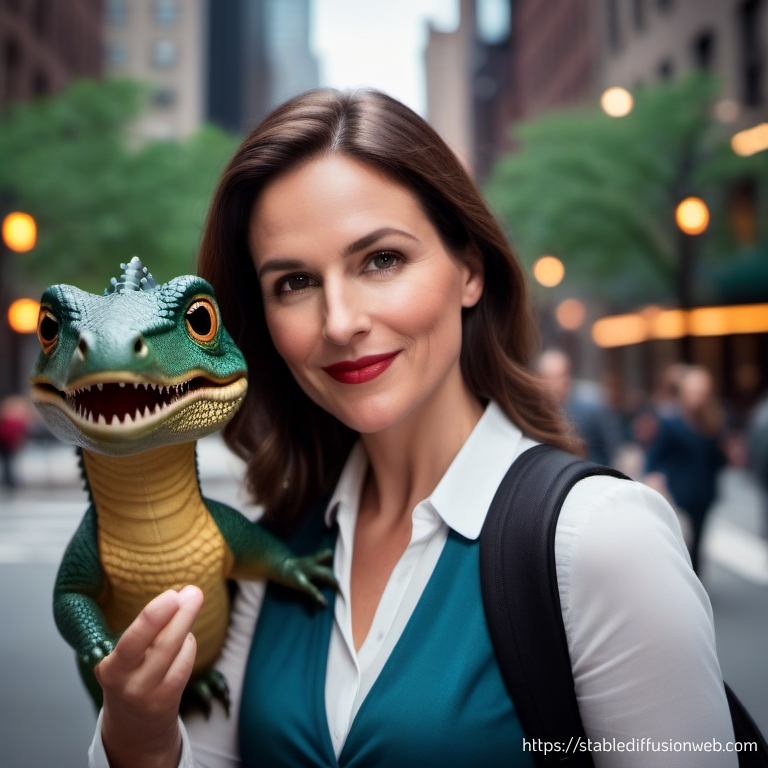
\includegraphics[width=7cm]{figs/selfie}
    \end{column}%
    \hfill%
    \begin{column}{.38\textwidth}
      {\small Stable Diffusion XL:} \\
      selfie of a teacher with a dinousar, in Manhattan \\
      cinematic-default \\
    \end{column}%
  \end{columns}

\end{frame}

%%-----------------------------------------
\begin{frame}[fragile]
  \frametitle{But beware!}

  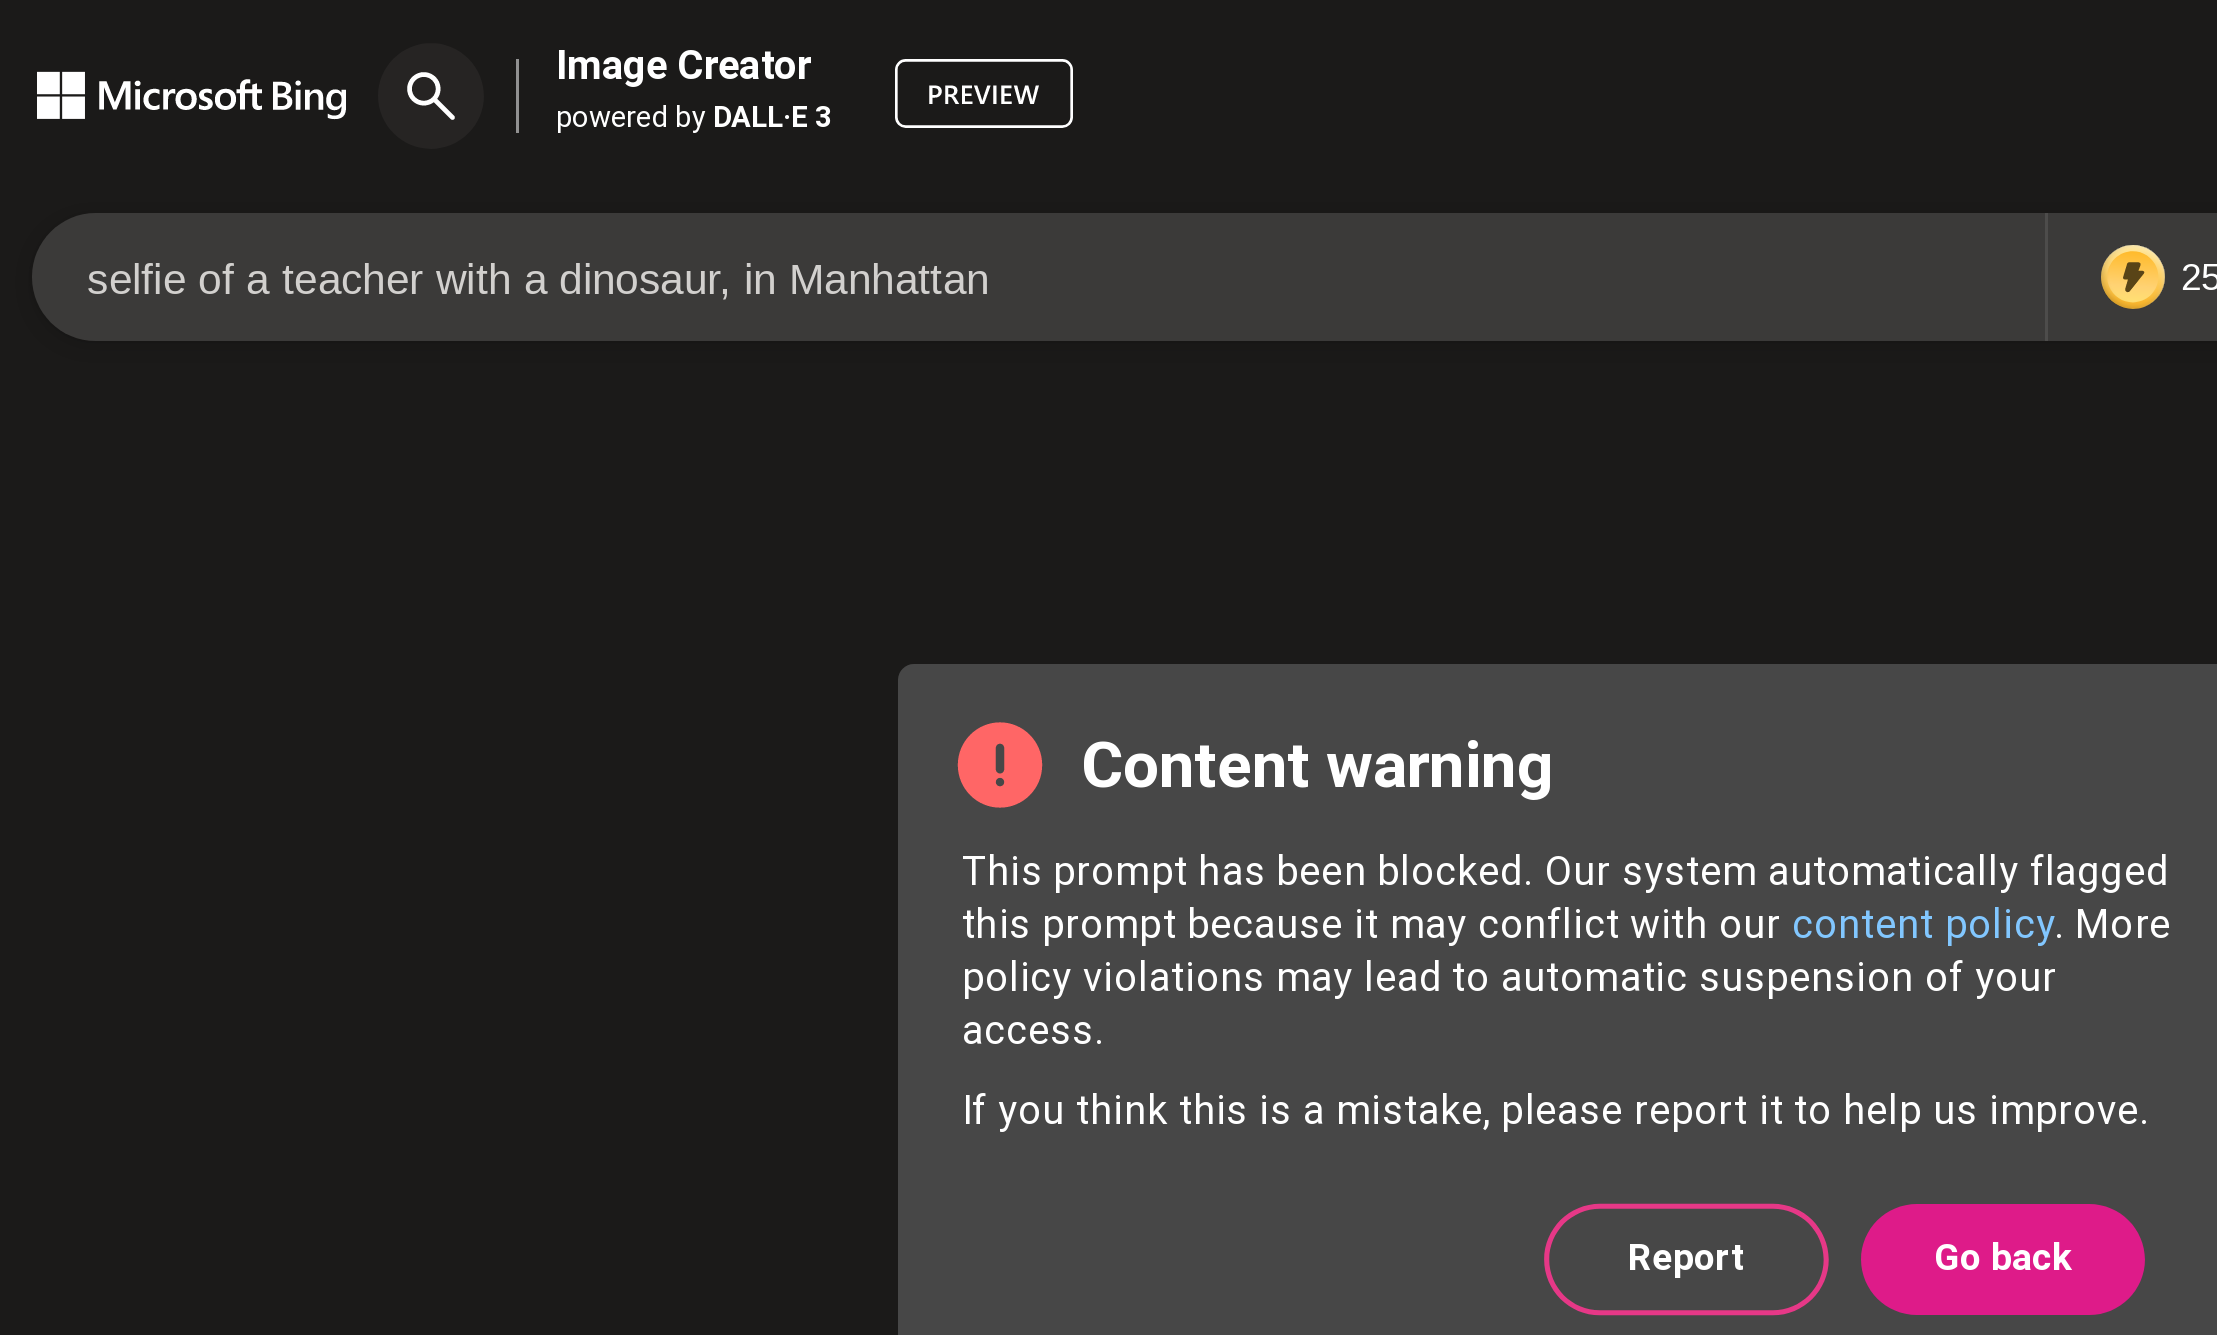
\includegraphics[width=6.5cm]{figs/bing-content-warning}

  {\small
  ``selfie of a teacher with a dinosaur, in Manhattan''
}  
\end{frame}

%%-----------------------------------------
\begin{frame}[fragile]

  {\Large
    Can we control \\
    how we use \\
    generative models? \\
  }  
\end{frame}

%%-----------------------------------------
\begin{frame}[fragile]
  \frametitle{What's a generative model}

  \begin{itemize}
  \item Architecture
  \item Weights, just weitghts
  \item Software to make inferences
  \end{itemize}

  But also:

  \begin{itemize}
  \item Data to train, benchmark
  \item Software to train, benchmark
  \item Weights of intermediate models
  \item Documentation, explaining everything
  \end{itemize}
\end{frame}



%% -----------------------------------------
\begin{frame}[fragile]
  \frametitle{Example: Stable Diffusion}

      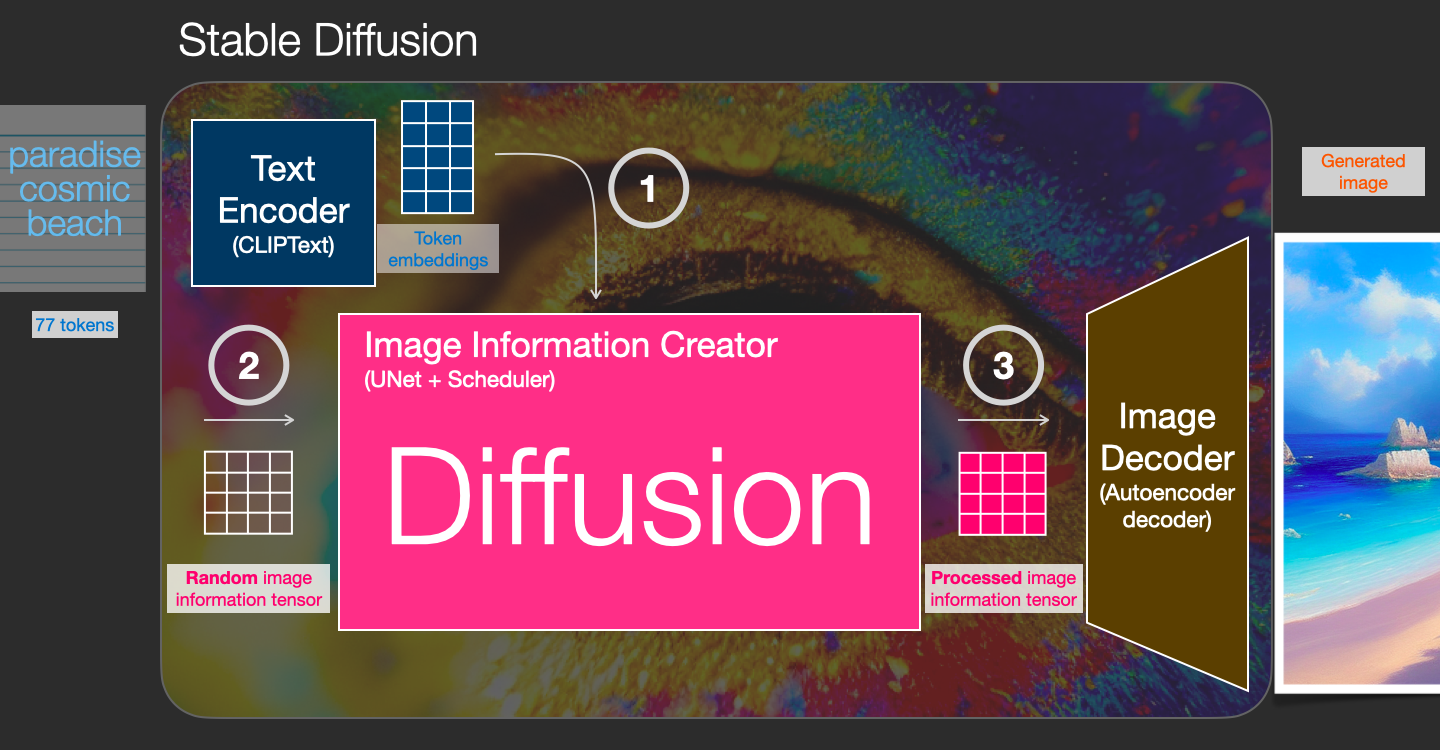
\includegraphics[width=10cm]{figs/sd-process}

  \begin{flushright}
    {\scriptsize
    \url{https://jalammar.github.io/illustrated-stable-diffusion/}
    }
  \end{flushright}

\end{frame}



%%-----------------------------------------
\begin{frame}[fragile]
\frametitle{}

  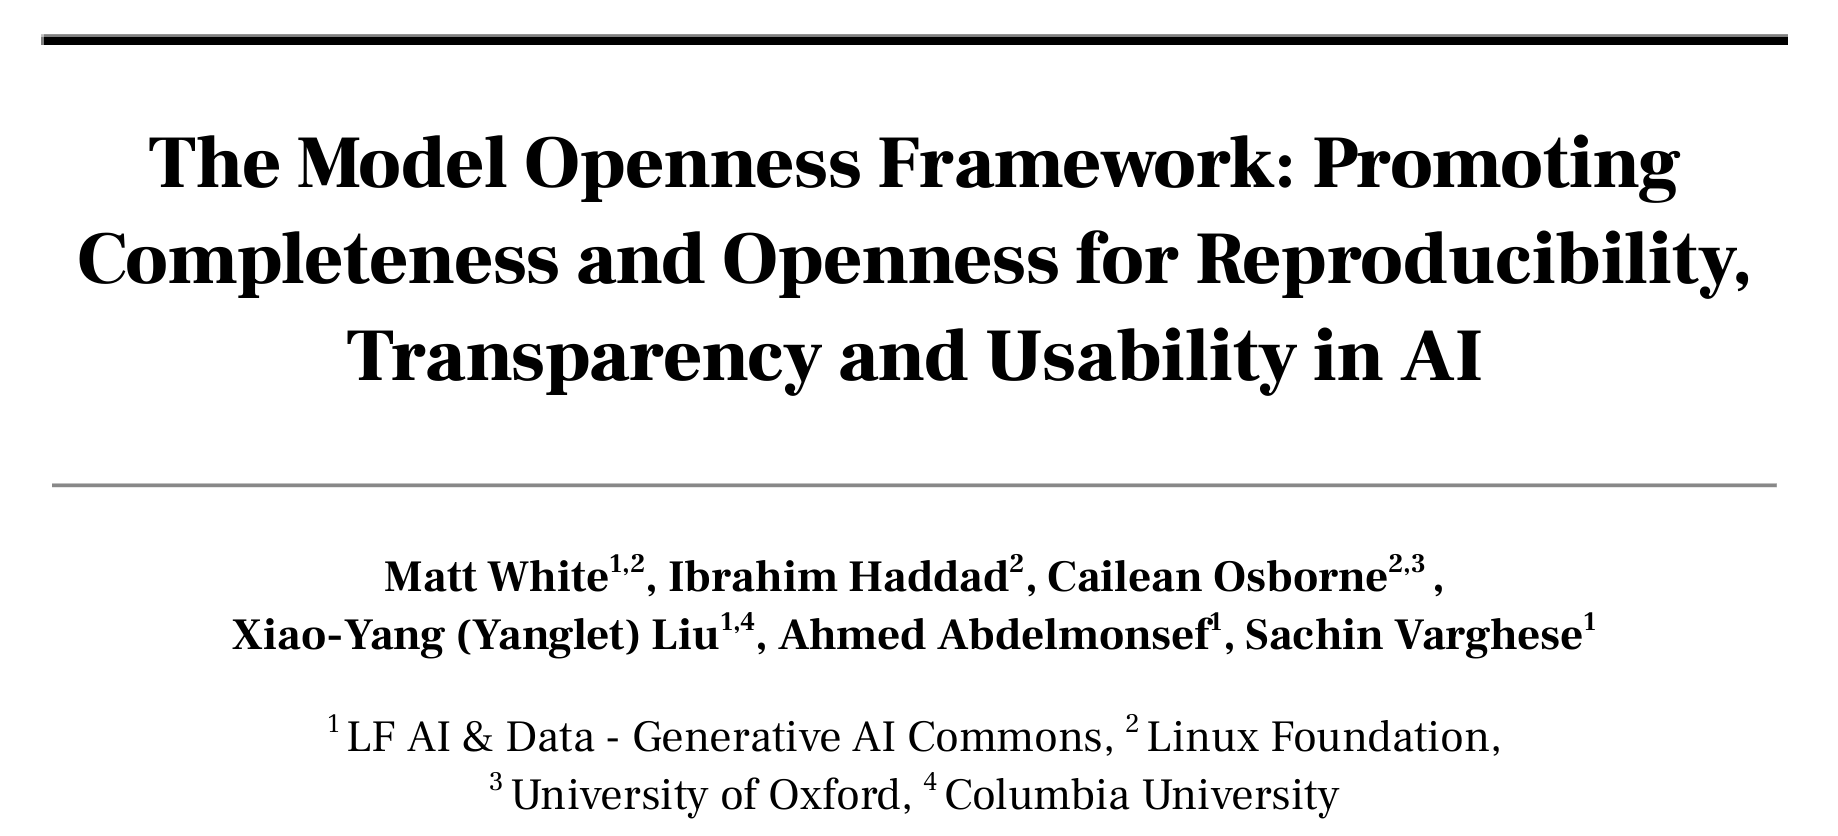
\includegraphics[height=6cm]{figs/paper-openess-framework}

  \begin{flushright}
    {\small
      \url{https://arxiv.org/abs/2403.13784}
    }
  \end{flushright} 

\end{frame}

%%-----------------------------------------
\begin{frame}[fragile]
\frametitle{Classes of ``openess''}

\begin{itemize}
\item Open science: paper, datasets, log files, intermediate models parameters \& metadata
\item Open tooling: training, inference, and evaluation code, libraries, evaluation data
\item Open model: architecture, model parameters \& medatadata, tech report, model card, data card
\end{itemize}

\end{frame}

%%-----------------------------------------
\begin{frame}[fragile]
\frametitle{For each of them...}

\begin{itemize}
\item Freedom of use
\item Freedom of study
\item Freedom of modification
\item Freedom of sharing
\end{itemize}
\end{frame}


%%-----------------------------------------
\begin{frame}[fragile]
\frametitle{Minimum for running in your computer}

\begin{itemize}
\item Inference code, with libraries
\item Model architecture
\item Model parameters \& metadata (weights)
\item Technical report (prompts, etc.)
\item Model card (convenient)
\end{itemize}

\end{frame}

%%-----------------------------------------
\begin{frame}[fragile]
\frametitle{Equipment requirements}

\begin{itemize}
\item Depends on architecture, and size of the model
\item CPU can be enough, GPU can accelerate a lot
\item RAM enough so that model fits
\item Code is usually FOSS
\end{itemize}

\end{frame}

%%-----------------------------------------
\begin{frame}[fragile]
\frametitle{Example: HuggingChat}

\begin{center}
  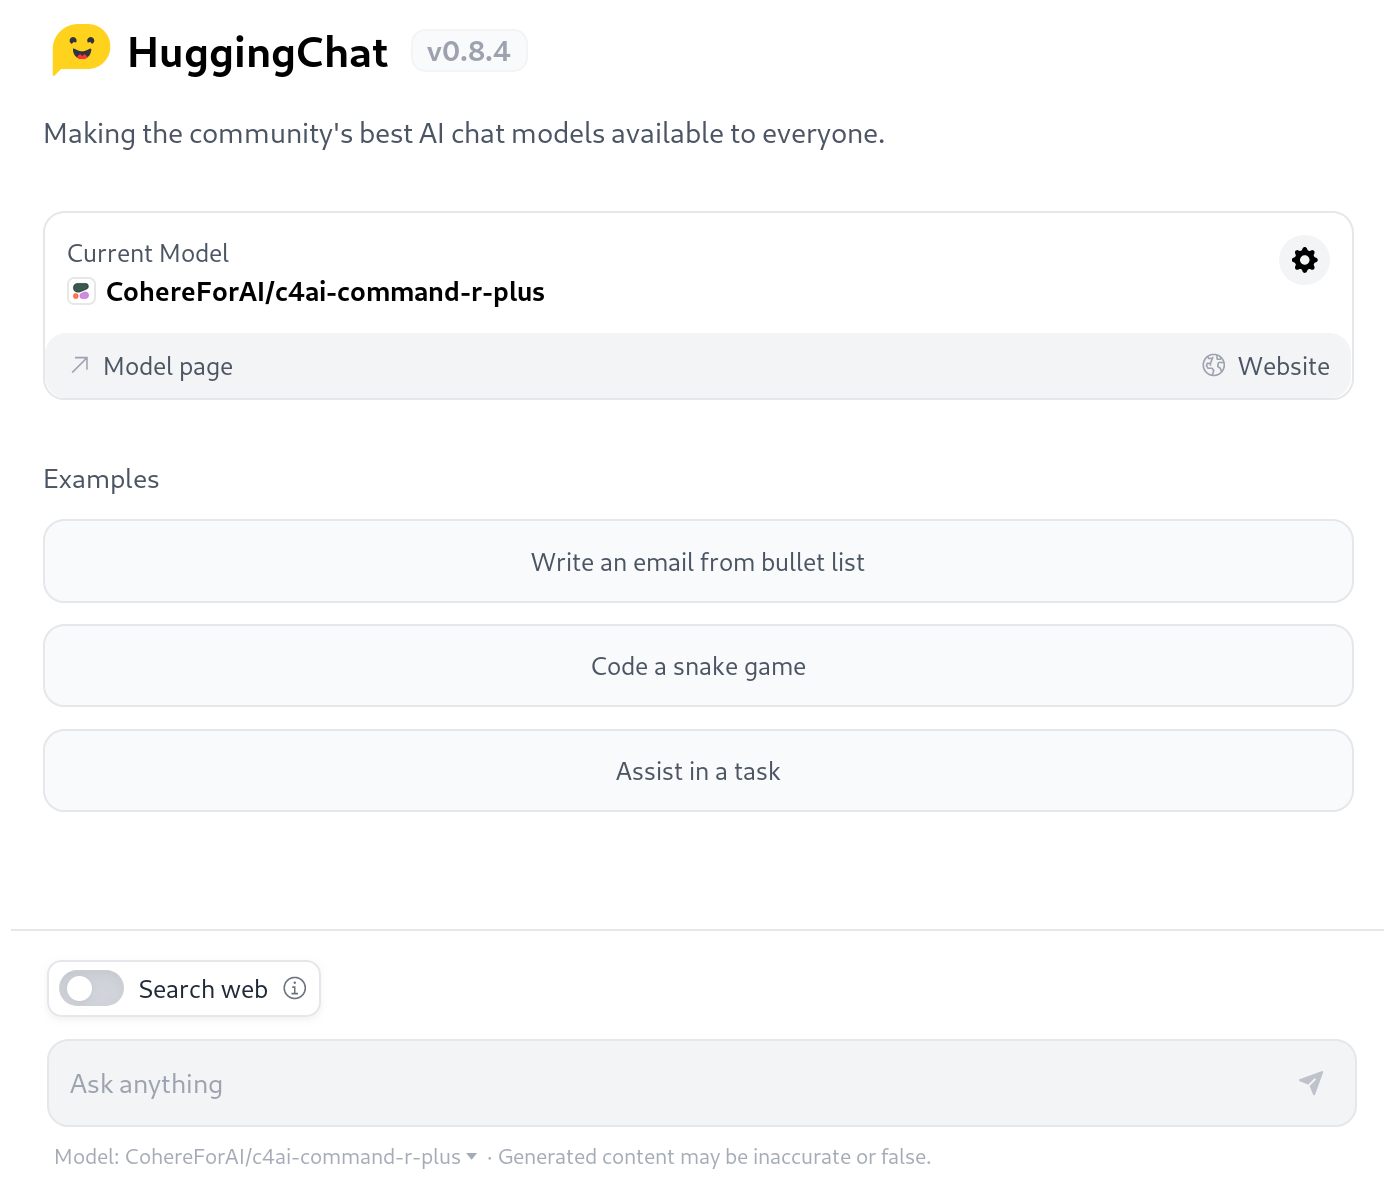
\includegraphics[width=6cm]{figs/huggingchat}
  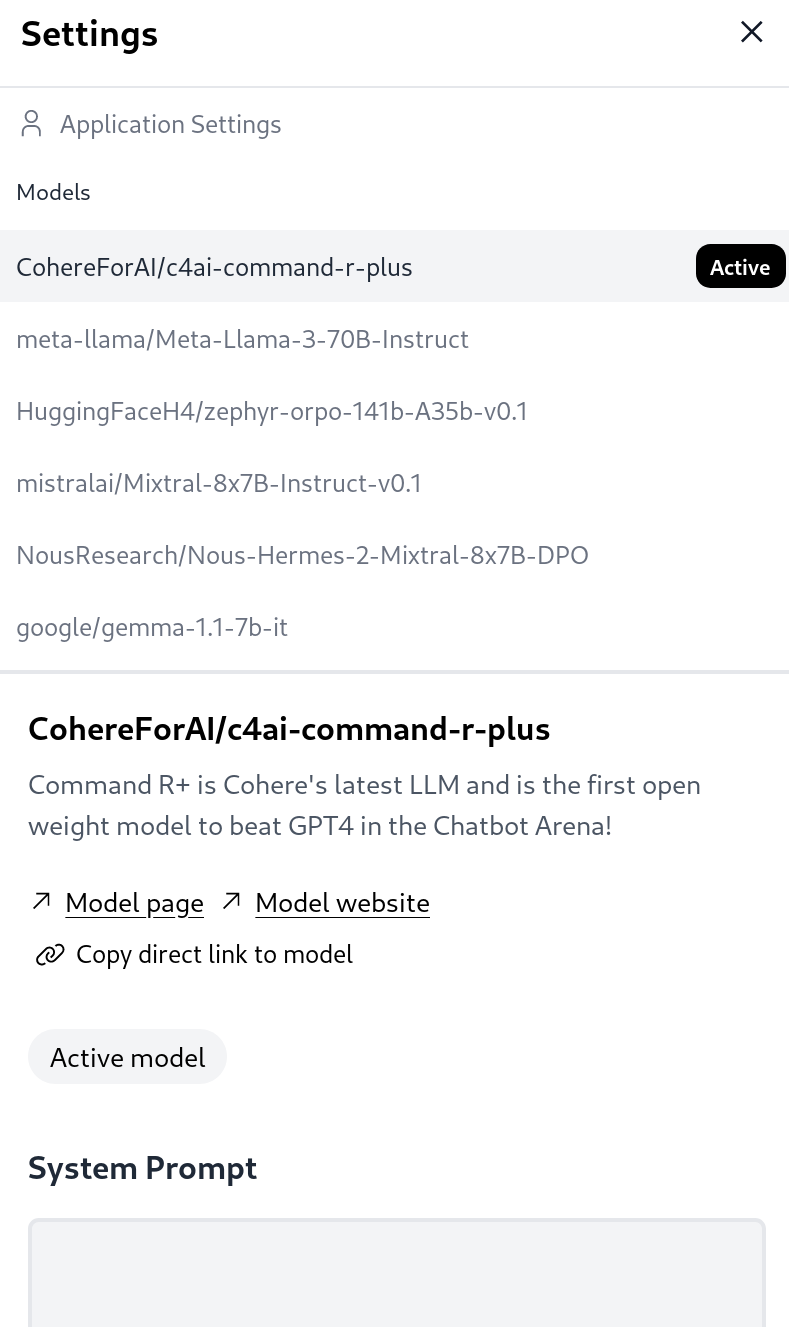
\includegraphics[width=3cm]{figs/huggingchat-models}
\end{center}

\begin{flushright}
  {\small
    \url{https://huggingface.co/chat/}
  }
\end{flushright}
\end{frame}

%%-----------------------------------------
\begin{frame}[fragile]
\frametitle{Example: Stable Diffusion}

\begin{center}
  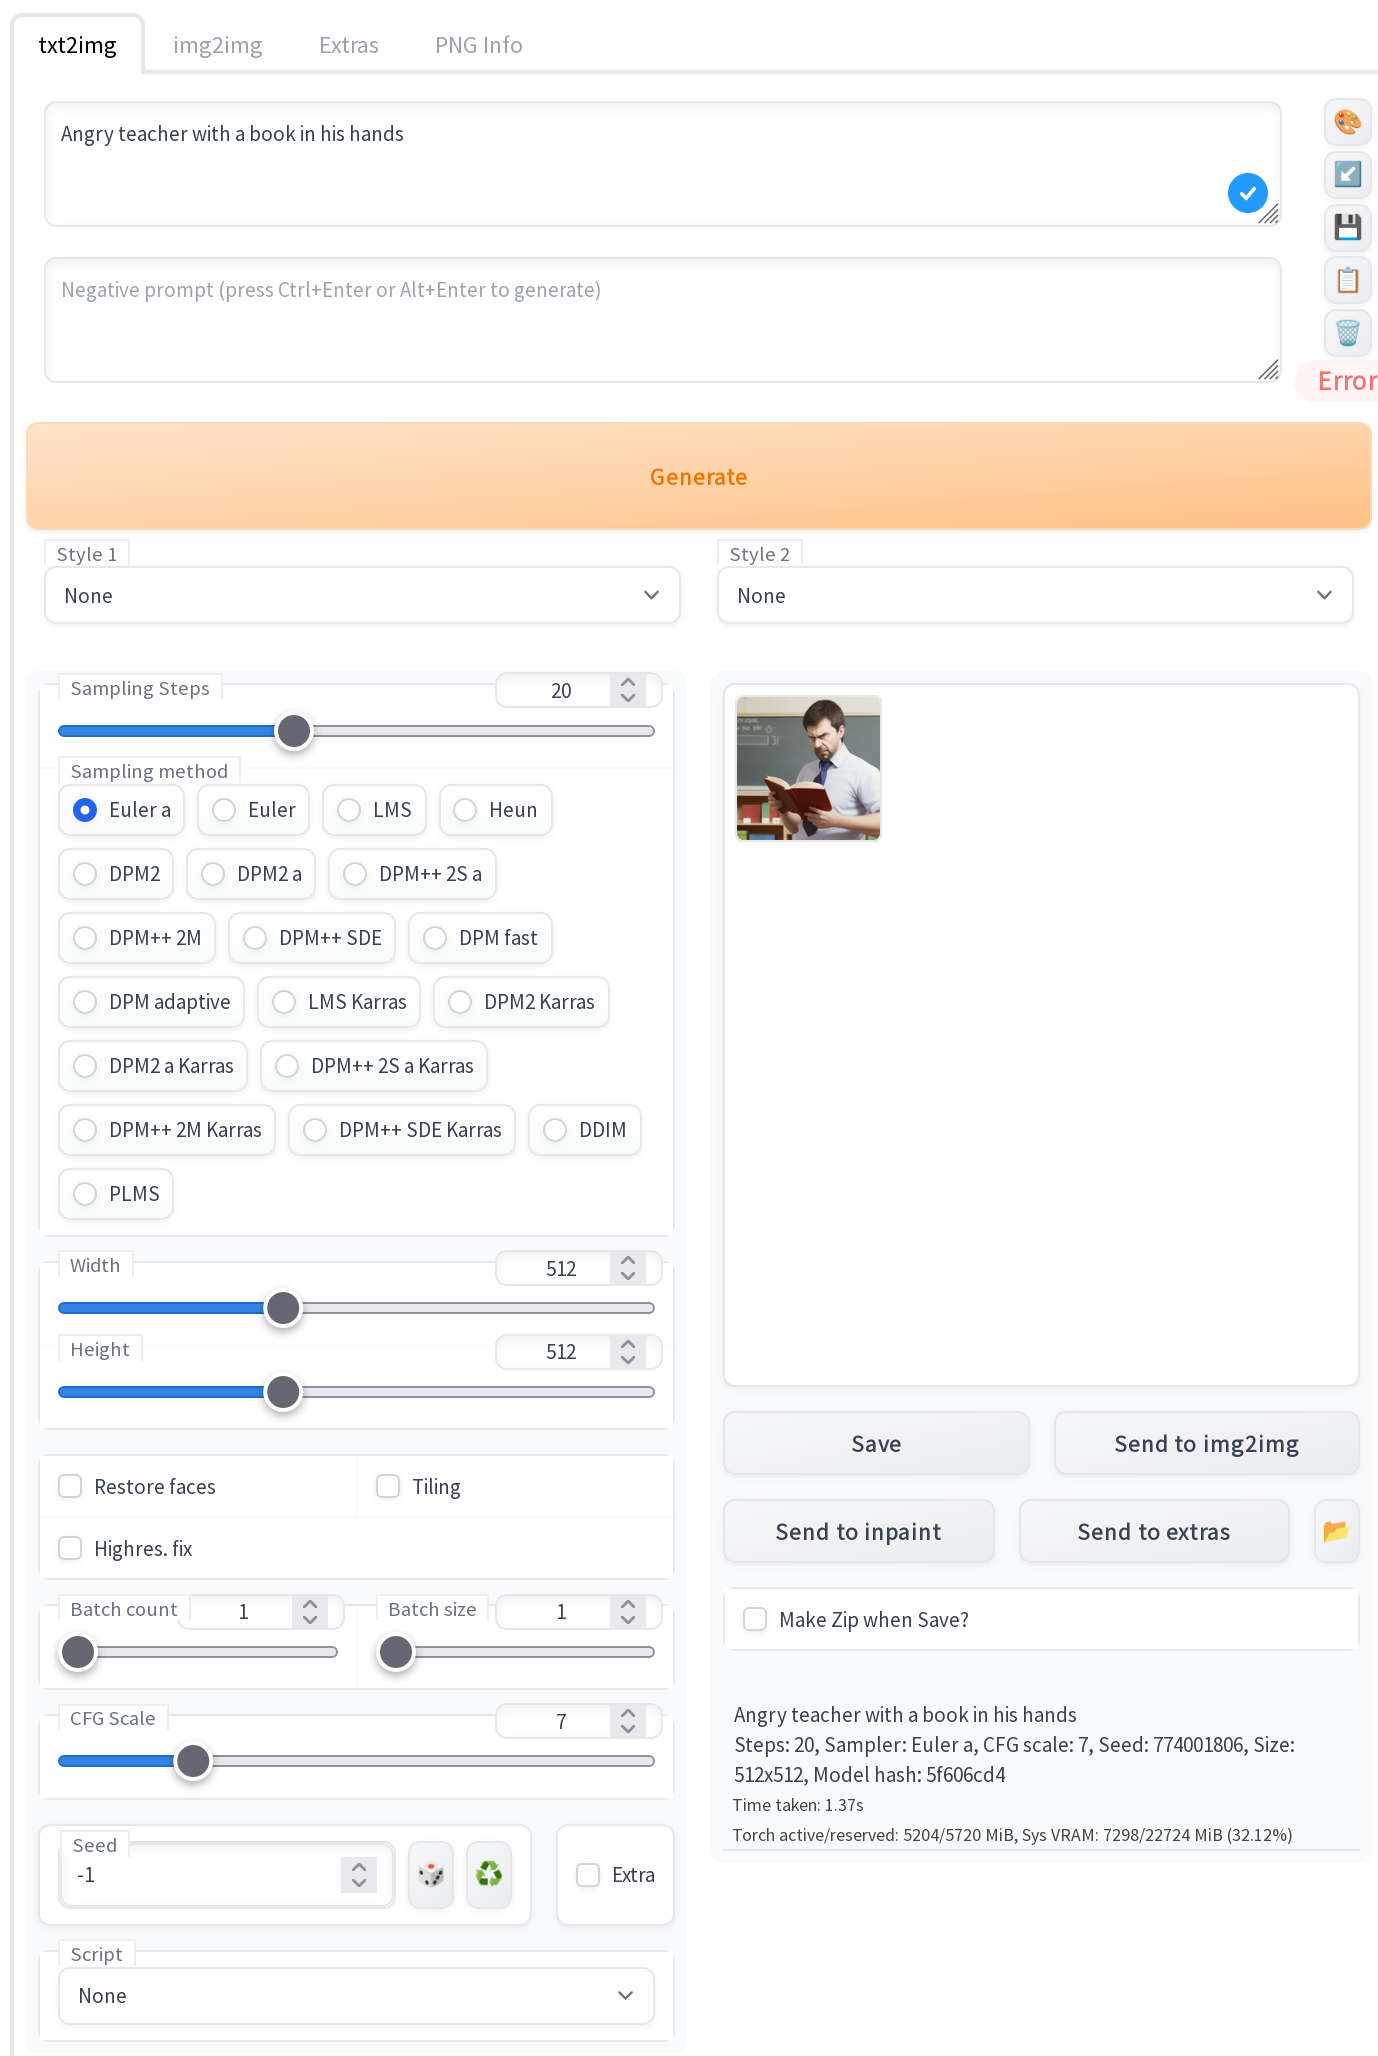
\includegraphics[width=5cm]{figs/protogen-webui}
\end{center}

\begin{flushright}
  {\small
    \url{https://huggingface.co/spaces/darkstorm2150/protogen-web-ui}
  }
\end{flushright}
\end{frame}

%%-----------------------------------------
\begin{frame}[fragile]
\frametitle{Example: TripoSR}

\begin{center}
  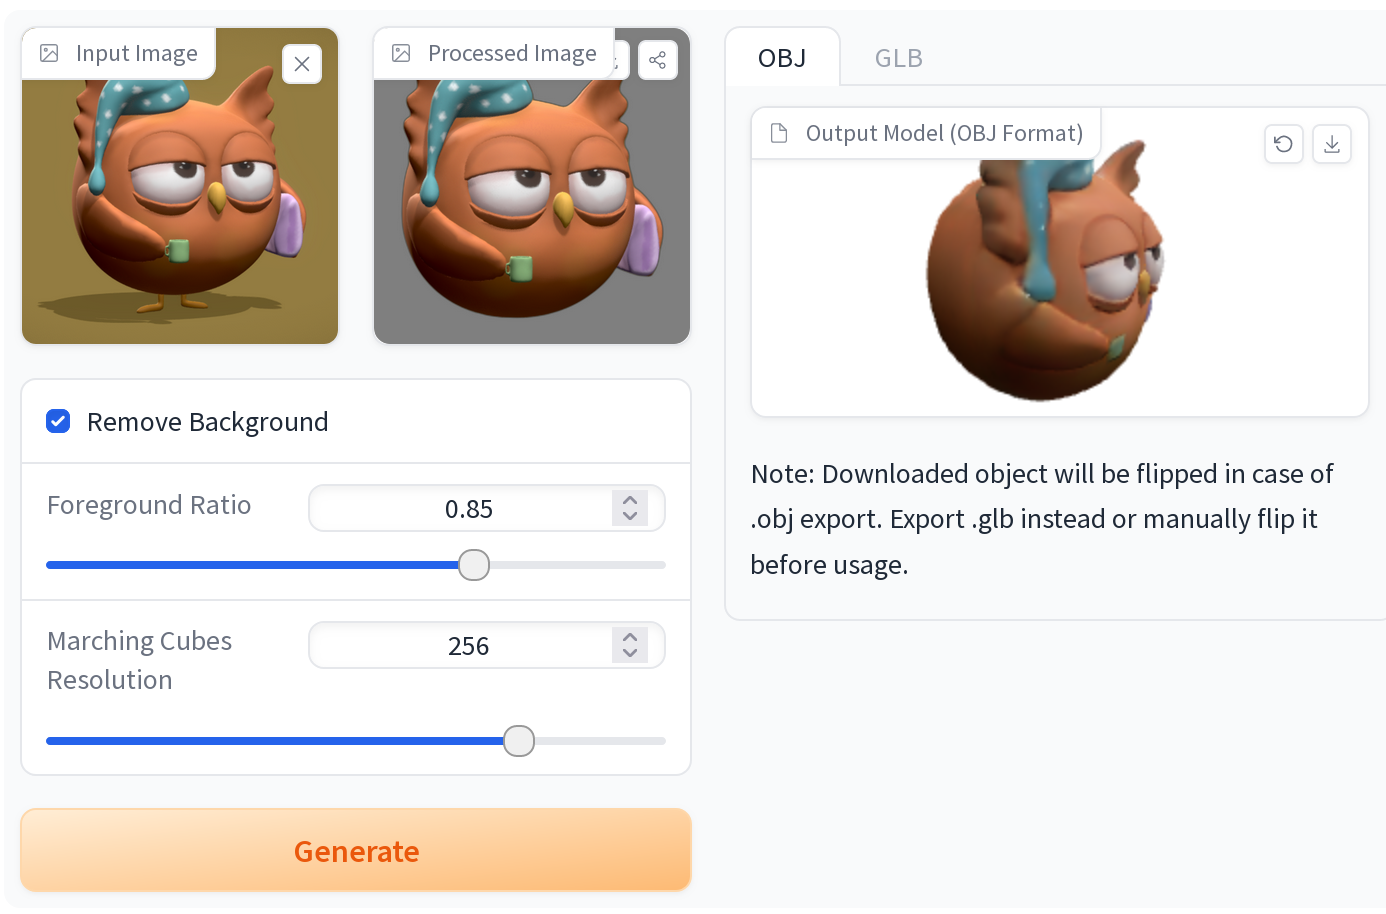
\includegraphics[width=5cm]{figs/triposr}
\end{center}

\begin{flushright}
  {\small
    \url{https://huggingface.co/spaces/stabilityai/TripoSR}
  }
\end{flushright}
\end{frame}

%%-----------------------------------------
%%-----------------------------------------
\section{Generative AI in your computer}

%%-----------------------------------------
\begin{frame}[fragile]
  \frametitle{Speech to text: Whisper}

%  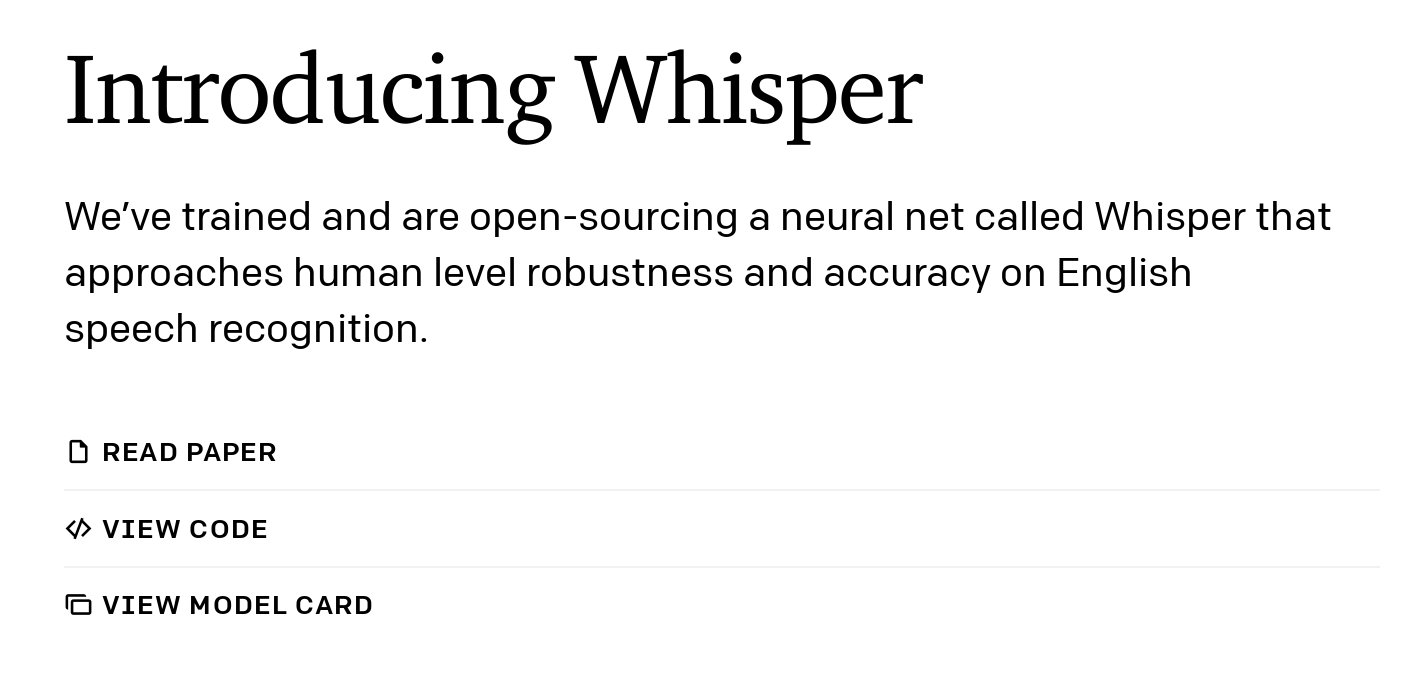
\includegraphics[width=8.5cm]{figs/whisper}
{\small
\begin{verbatim}
#!/usr/bin/python3
import whisper

model = whisper.load_model('tiny')
transcription = model.transcribe('recording.wav')
print(transcription['text'])
\end{verbatim}
}

\begin{verbatim}
$ whisper speech.wav --language Spanish
\end{verbatim}

\begin{flushright}
  {\scriptsize
    \url{https://openai.com/blog/whisper/} \\
    \url{https://github.com/openai/whisper} \\
    License: MIT (open source) \\
  }
\end{flushright}

\end{frame}

%%-----------------------------------------
\begin{frame}[fragile]
  \frametitle{Text to speech: Coqui TTS}

{\small
\begin{verbatim}
$ tts --text "Texto" \
  --model_name tts_models/es/mai/tacotron2-DDC \
  --out_path speech.wav
\end{verbatim}
}

  \begin{flushright}
    {\small
    \url{https://github.com/idiap/coqui-ai-TTS} \\
    License: MPL-2.0 (open source) \\
  }
  \end{flushright}

\end{frame}


%% -----------------------------------------
\begin{frame}[fragile]
\frametitle{Stable Diffussion}

EasyDiffusion:
\begin{flushright}
\url{https://easydiffusion.github.io}
\end{flushright}

Fooocus:
\begin{flushright}
\url{https://github.com/lllyasviel/Fooocus}
\end{flushright}

AUTOMATIC1111:
\begin{flushright}
\url{https://github.com/AUTOMATIC1111/stable-diffusion-webui}
\end{flushright}

\end{frame}

%% -----------------------------------------
\begin{frame}[fragile]
\frametitle{Stable Diffussion (2)}

SD.next:
\begin{flushright}
\url{https://github.com/vladmandic/automatic}
\end{flushright}

ComfyUI:
\begin{flushright}
\url{https://github.com/comfyanonymous/ComfyUI}
\end{flushright}

\end{frame}

%% -----------------------------------------
\begin{frame}[fragile]
\frametitle{Text generation models}

Llama3 (70b, 8b), Llama Community License
\begin{flushright}
  \url{https://llama.meta.com/llama3/} \\
  \url{https://github.com/meta-llama/llama3} \\
\end{flushright}

Command R+,  CC by-nc 4.0

\begin{flushright}
  \url{https://cohere.com/command}
  \url{https://huggingface.co/spaces/CohereForAI/c4ai-command-r-plus}
\end{flushright}

\end{frame}

%% -----------------------------------------
\begin{frame}[fragile]
\frametitle{Text generation models (2)}

Mixtral (8x22b, 8x7b), Apache 2.0

\begin{flushright}
  \url{https://mistral.ai/news/mixtral-8x22b/}
  \url{https://huggingface.co/mistralai/Mixtral-8x7B-v0.1}
\end{flushright}


Zephyr ORPO 141B-A39B, Apache 2.0

\begin{flushright}
  \url{https://huggingface.co/HuggingFaceH4/zephyr-orpo-141b-A35b-v0.1}
\end{flushright}

\end{frame}


%% -----------------------------------------
\begin{frame}[fragile]
\frametitle{Leaderboard}

    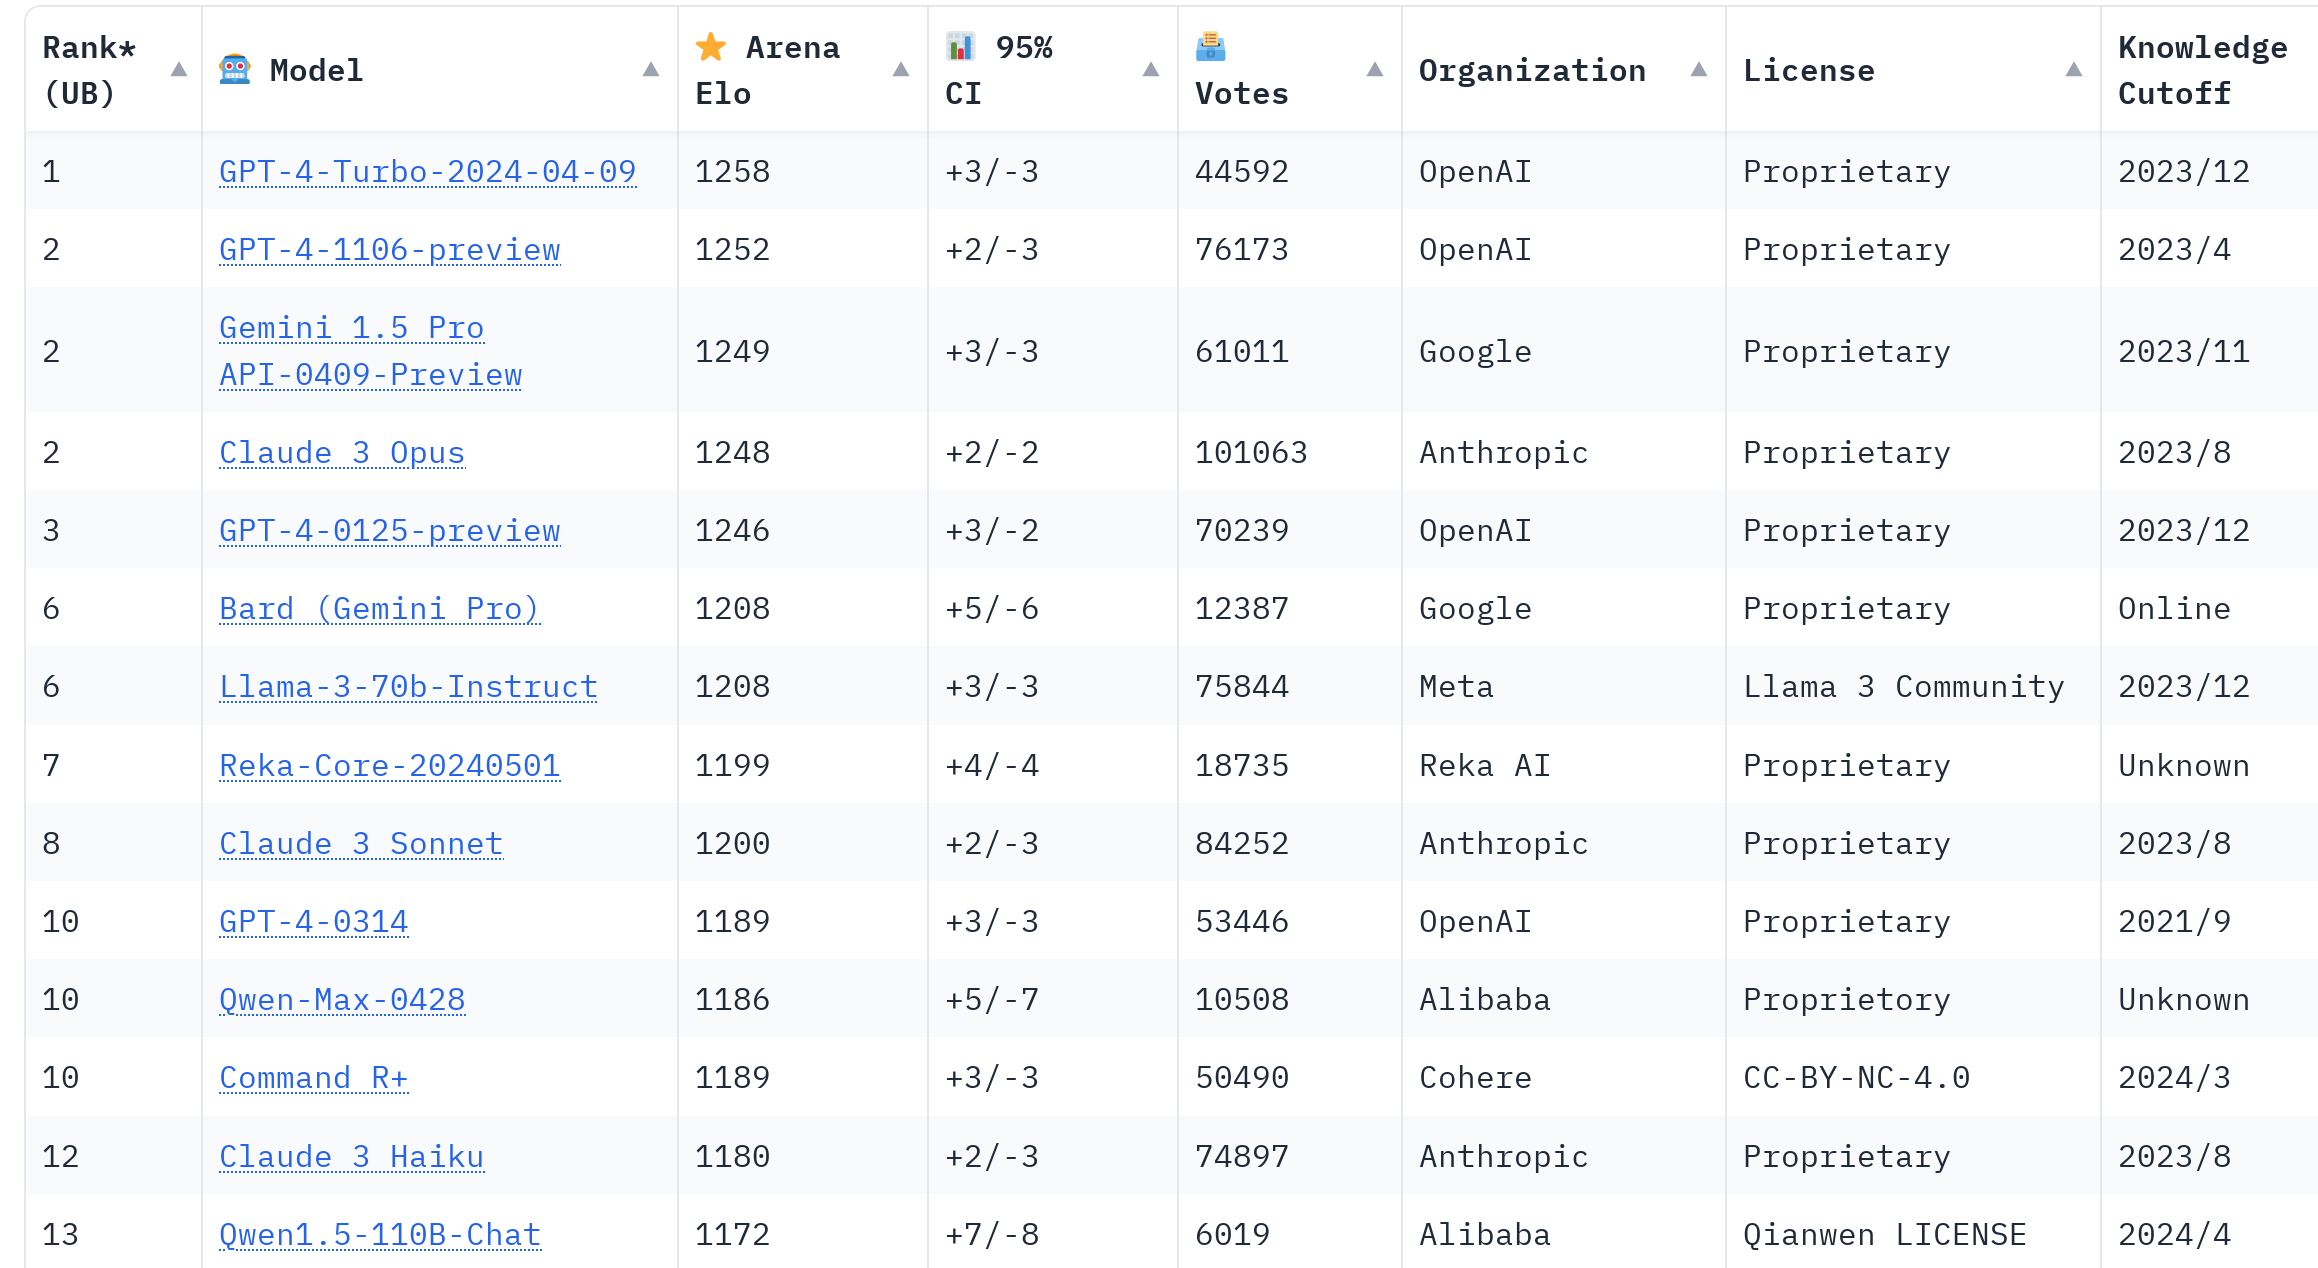
\includegraphics[width=7cm]{figs/leaderboard}


\url{https://chat.lmsys.org/?leaderboard}

\end{frame}


%% -----------------------------------------
\begin{frame}[fragile]
\frametitle{Inference engines}

llama.cpp

\begin{flushright}
  \url{https://github.com/ggerganov/llama.cpp}
\end{flushright}

Ollama

\begin{flushright}
  \url{https://ollama.com/}
\end{flushright}

vLLM

\begin{flushright}
  \url{https://github.com/vllm-project/vllm}
\end{flushright}


\end{frame}


%% -----------------------------------------
\begin{frame}[fragile]
\frametitle{Chat frontends}

Oobabooga:
\begin{flushright}
\url{https://github.com/oobabooga/text-generation-webui}
\end{flushright}

openplayground:
\begin{flushright}
\url{https://github.com/nat/openplayground}
\end{flushright}

catAI
\begin{flushright}
\url{https://github.com/withcatai/catai}
\end{flushright}

\end{frame}


%%-----------------------------------------
\begin{frame}[fragile]
  \frametitle{Collections of consented, open data}

  Chatbot Arena Leaderboard \\
  \url{https://chat.lmsys.org/}

  LAION Open Empathic \\
  \url{https://laion.ai/blog/open-empathic/}

  LAION Datasets \\
  \url{https://laion.ai/projects/}
\end{frame}



%%-----------------------------------------
%%-----------------------------------------
\section{Extending, combining}

%%-----------------------------------------
\begin{frame}[fragile]
  \frametitle{Integration: GIMP}

    \begin{center}
    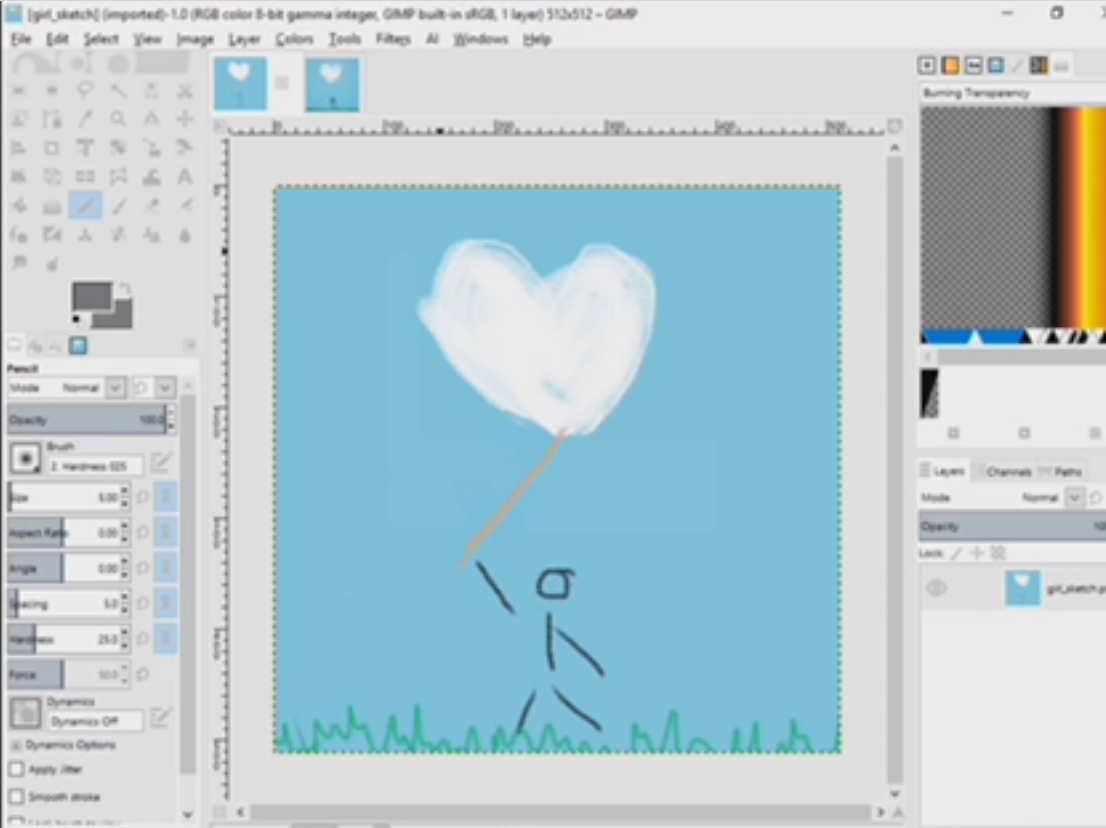
\includegraphics[width=7cm]{figs/sd-gimp}
  \end{center}

  \begin{flushright}
    {\scriptsize
    \url{https://github.com/blueturtleai/gimp-stable-diffusion} \\
    }
  \end{flushright}
  
\end{frame}

%%-----------------------------------------
\begin{frame}[fragile]
  \frametitle{Integration: Blender}

    \begin{center}
    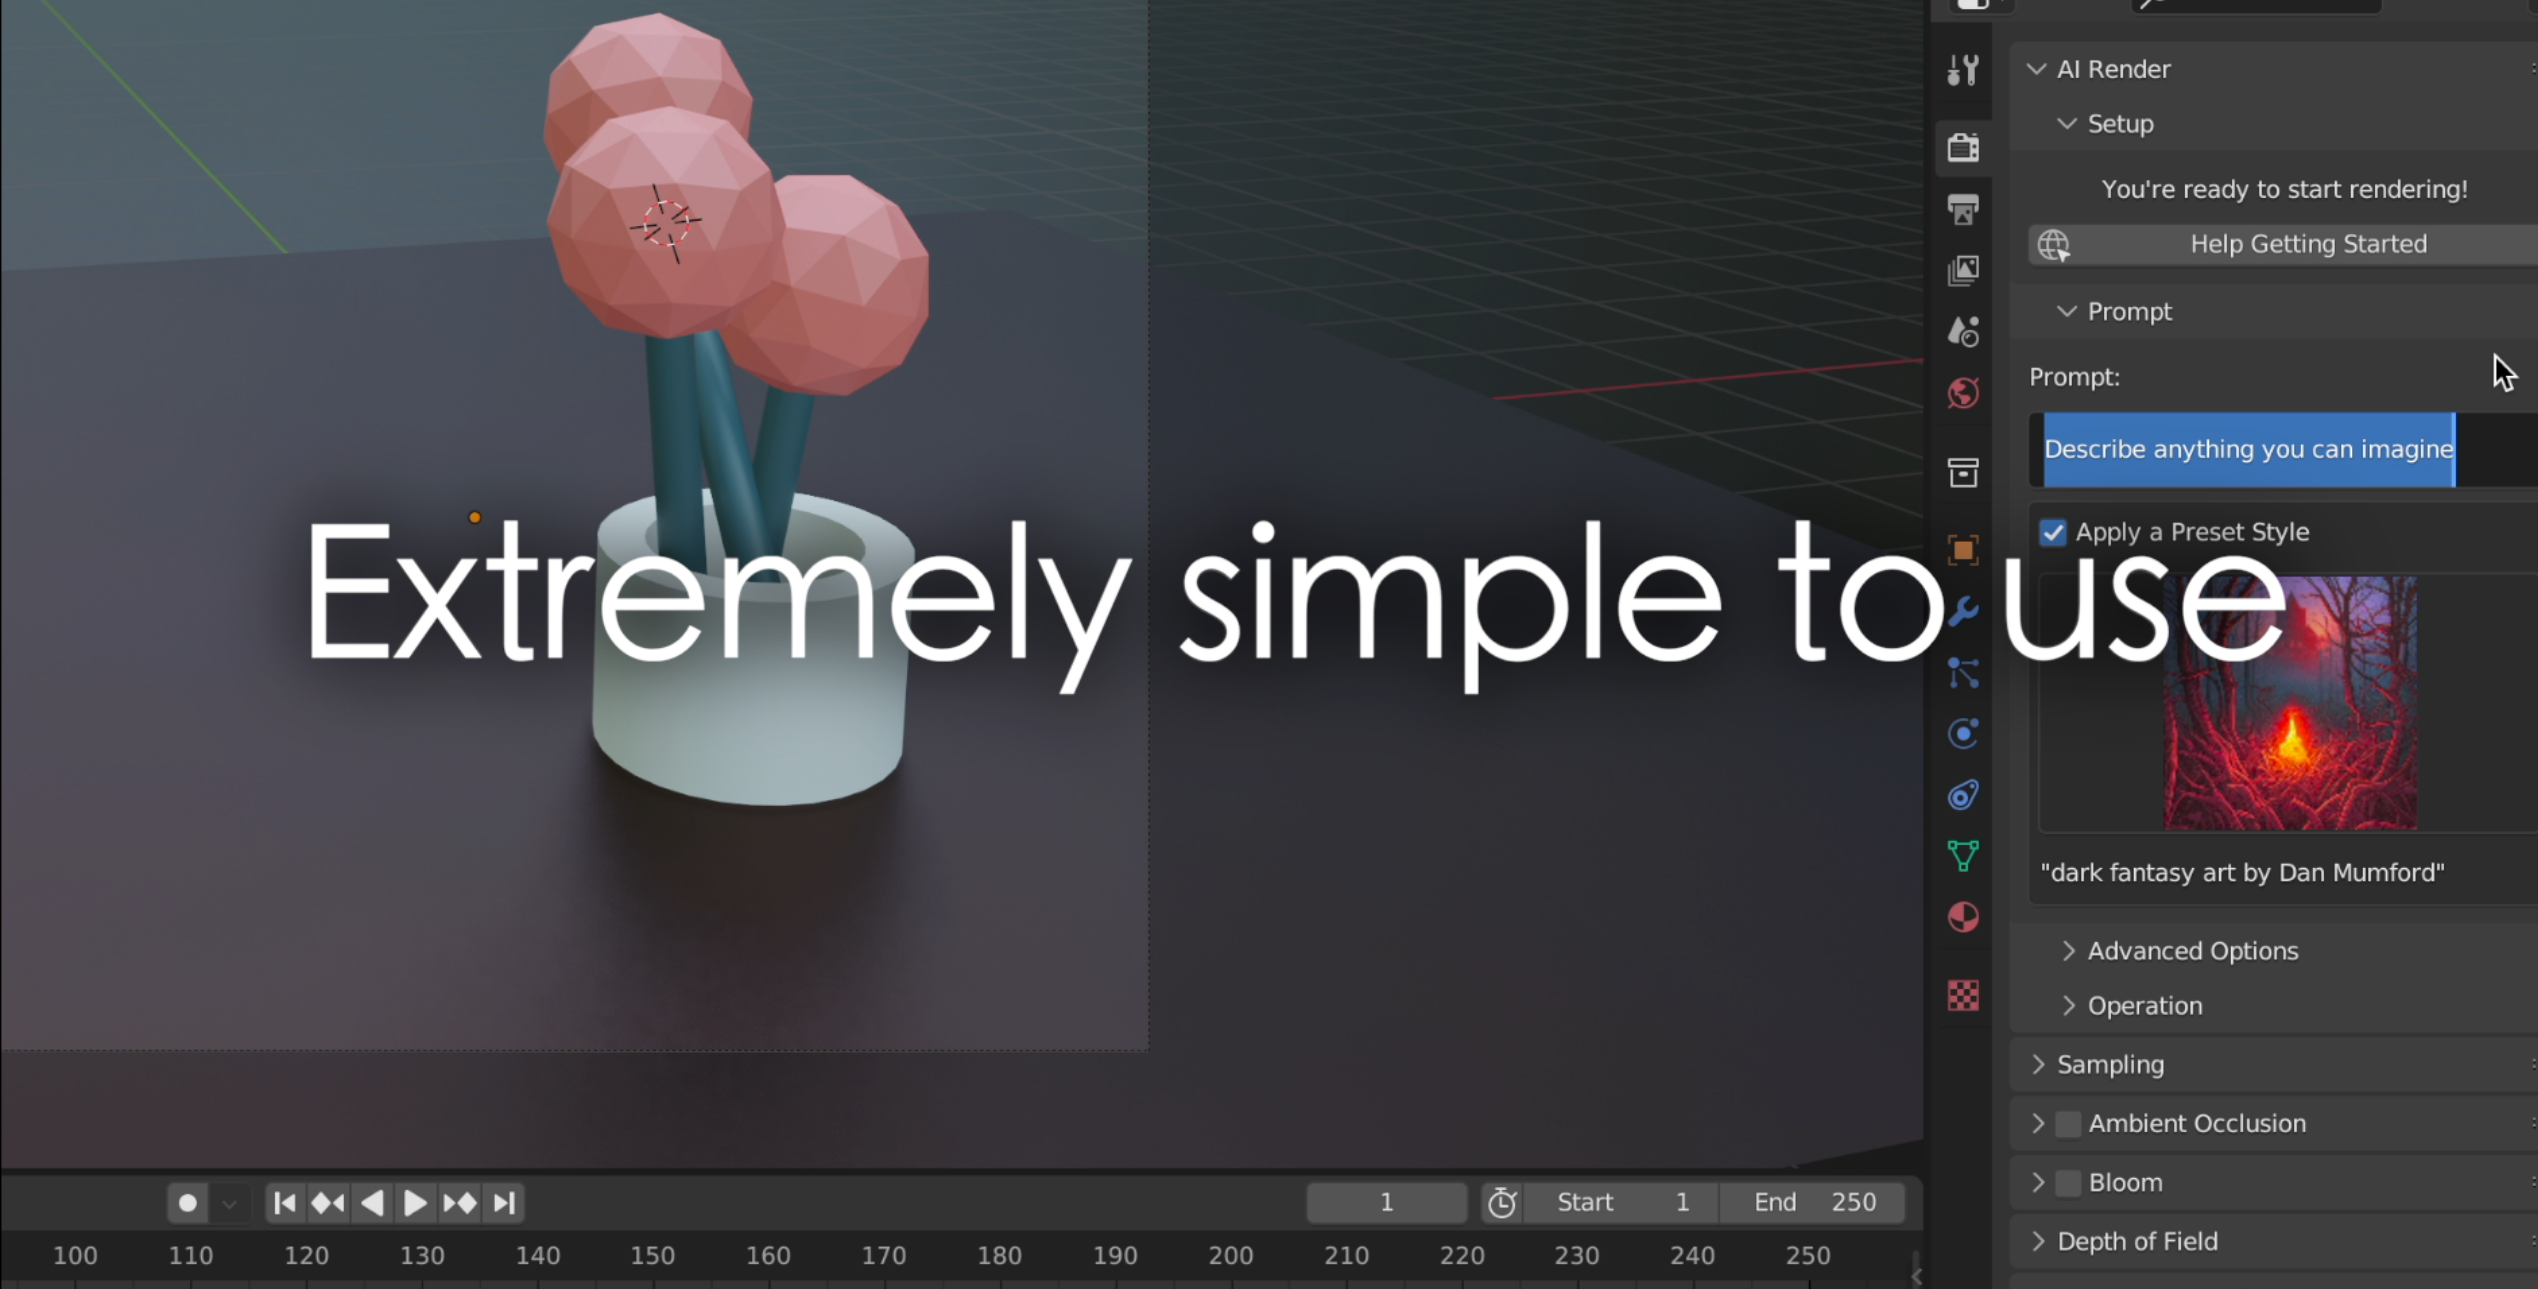
\includegraphics[width=7cm]{figs/sd-blender}
  \end{center}

  \begin{flushright}
    {\scriptsize
    \url{https://blendermarket.com/products/ai-render} \\
    }
  \end{flushright}
  
\end{frame}

%%-----------------------------------------
\begin{frame}[fragile]
  \frametitle{In-painting}

    \begin{center}
    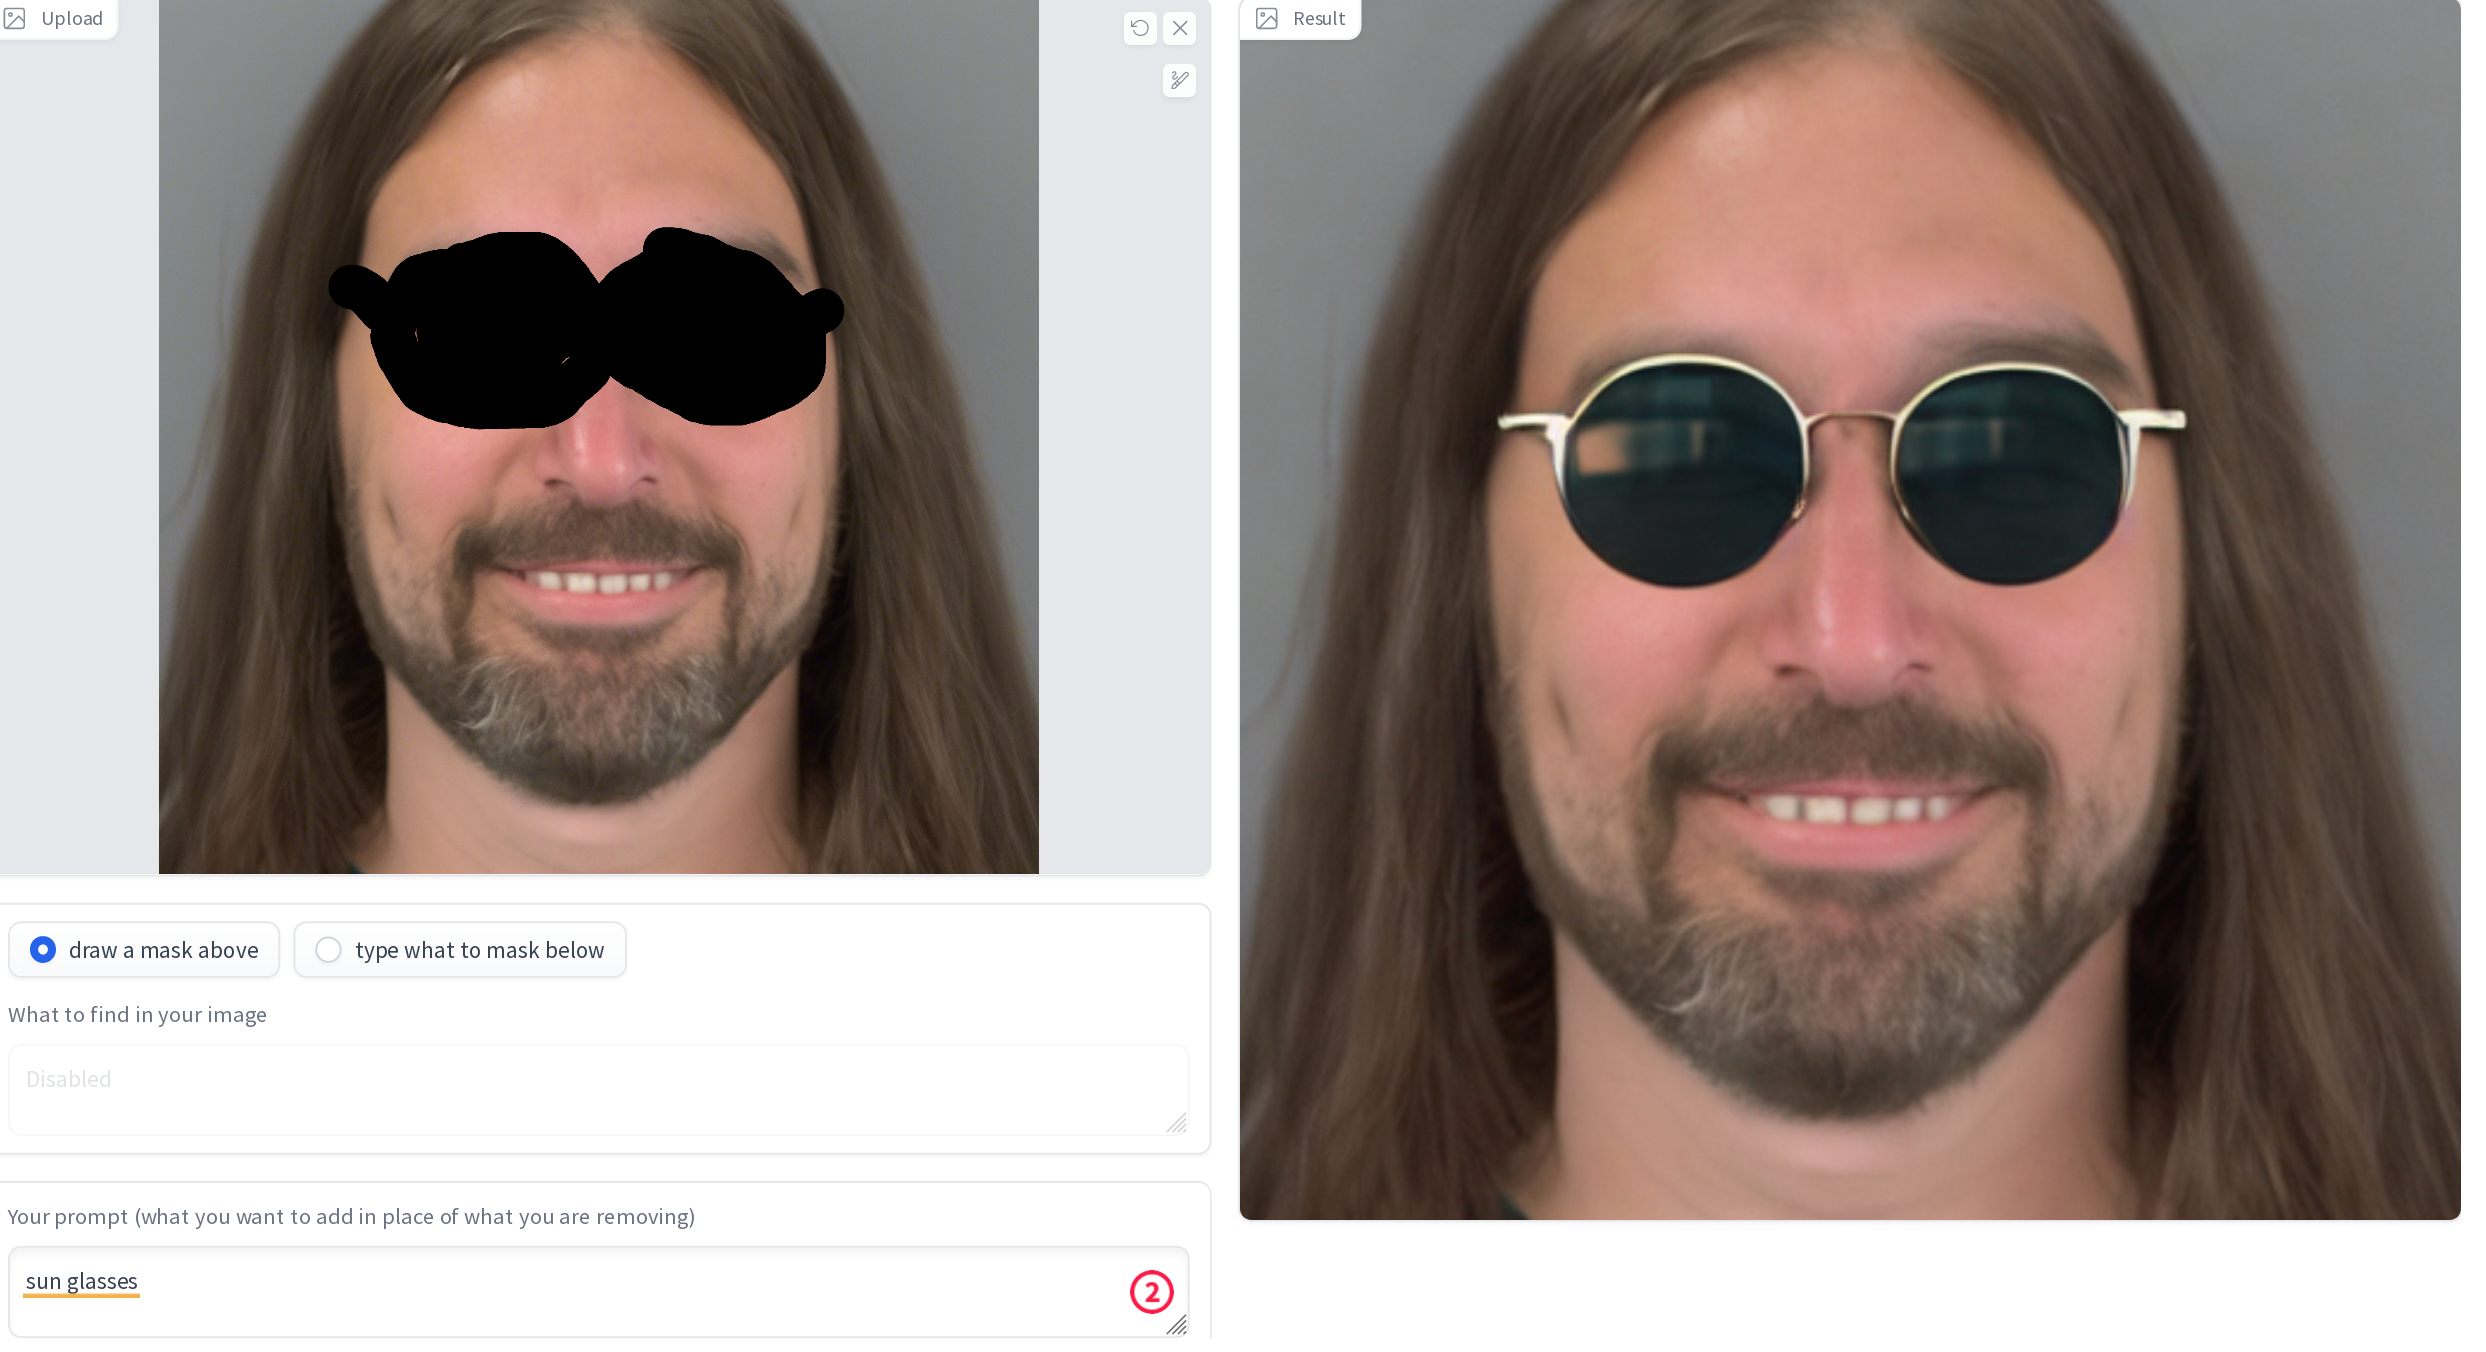
\includegraphics[width=9.5cm]{figs/sd-inpainting}
  \end{center}

  \begin{flushright}
    {\scriptsize
    \url{https://huggingface.co/spaces/multimodalart/stable-diffusion-inpainting} \\
    }
  \end{flushright}
  
\end{frame}

%%-----------------------------------------
\begin{frame}[fragile]
  \frametitle{Out-painting}

    \begin{center}
    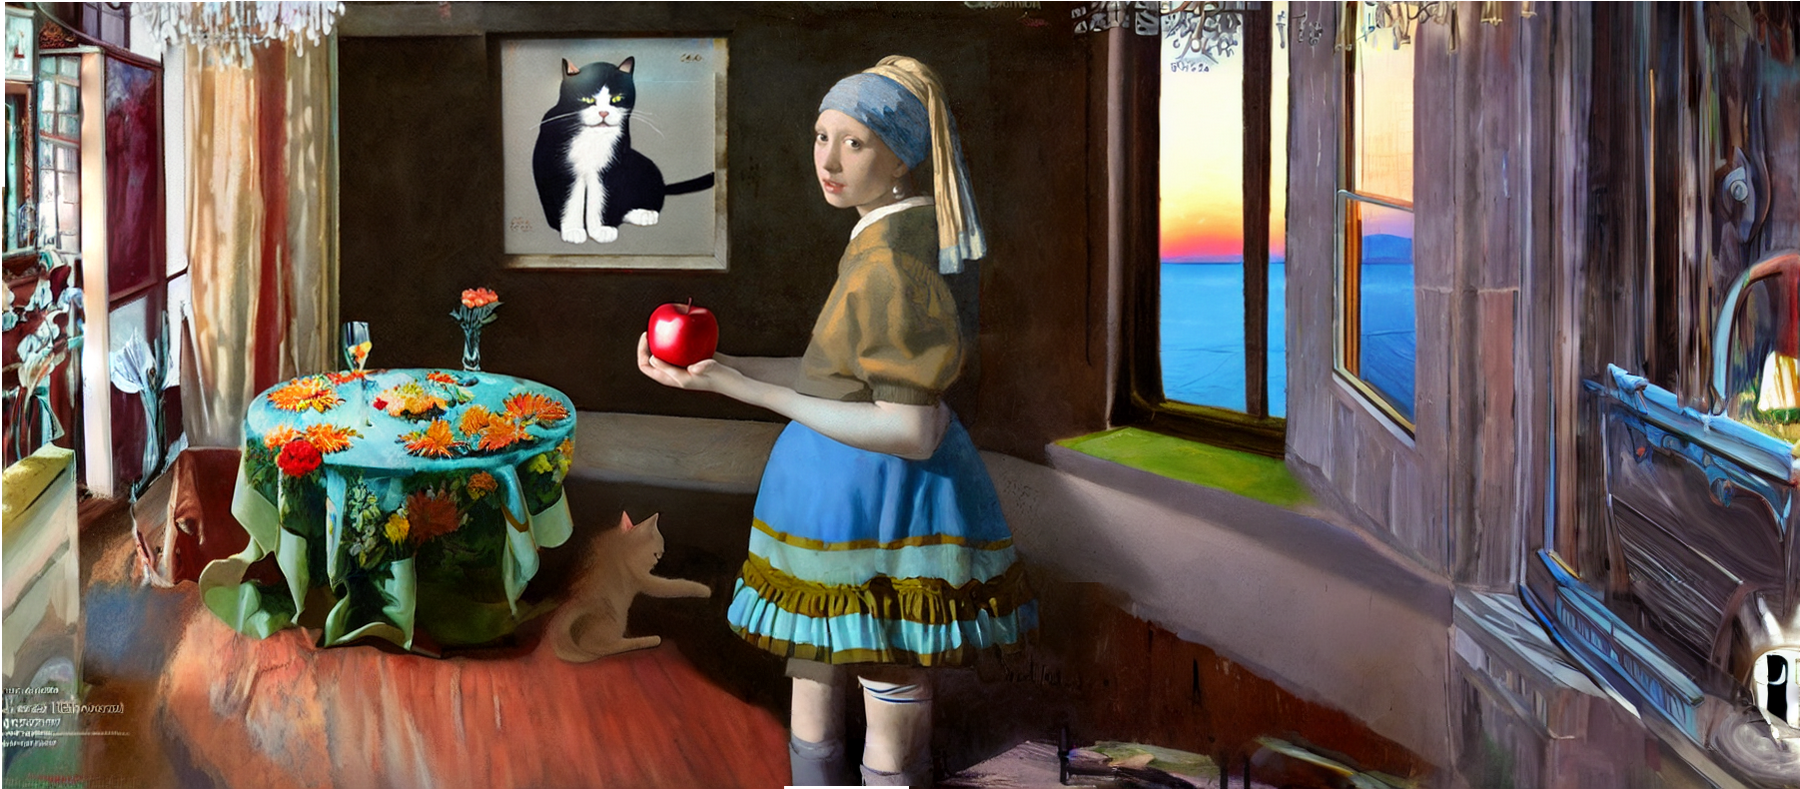
\includegraphics[width=9.5cm]{figs/sd-infinity}
  \end{center}

  \begin{flushright}
    {\scriptsize
    \url{https://github.com/lkwq007/stablediffusion-infinity} \\
    }
  \end{flushright}


  
  
\end{frame}


%% -----------------------------------------
\begin{frame}[fragile]
  \frametitle{Image to image}

  Image + prompt produces an image \\
  Even just with CPU! \\
  
  \begin{flushright}
    {\scriptsize
    \url{https://huggingface.co/spaces/fffiloni/stable-diffusion-img2img} \\
    }
  \end{flushright}
  
\end{frame}

%%-----------------------------------------
\begin{frame}[fragile]

  \begin{center}
    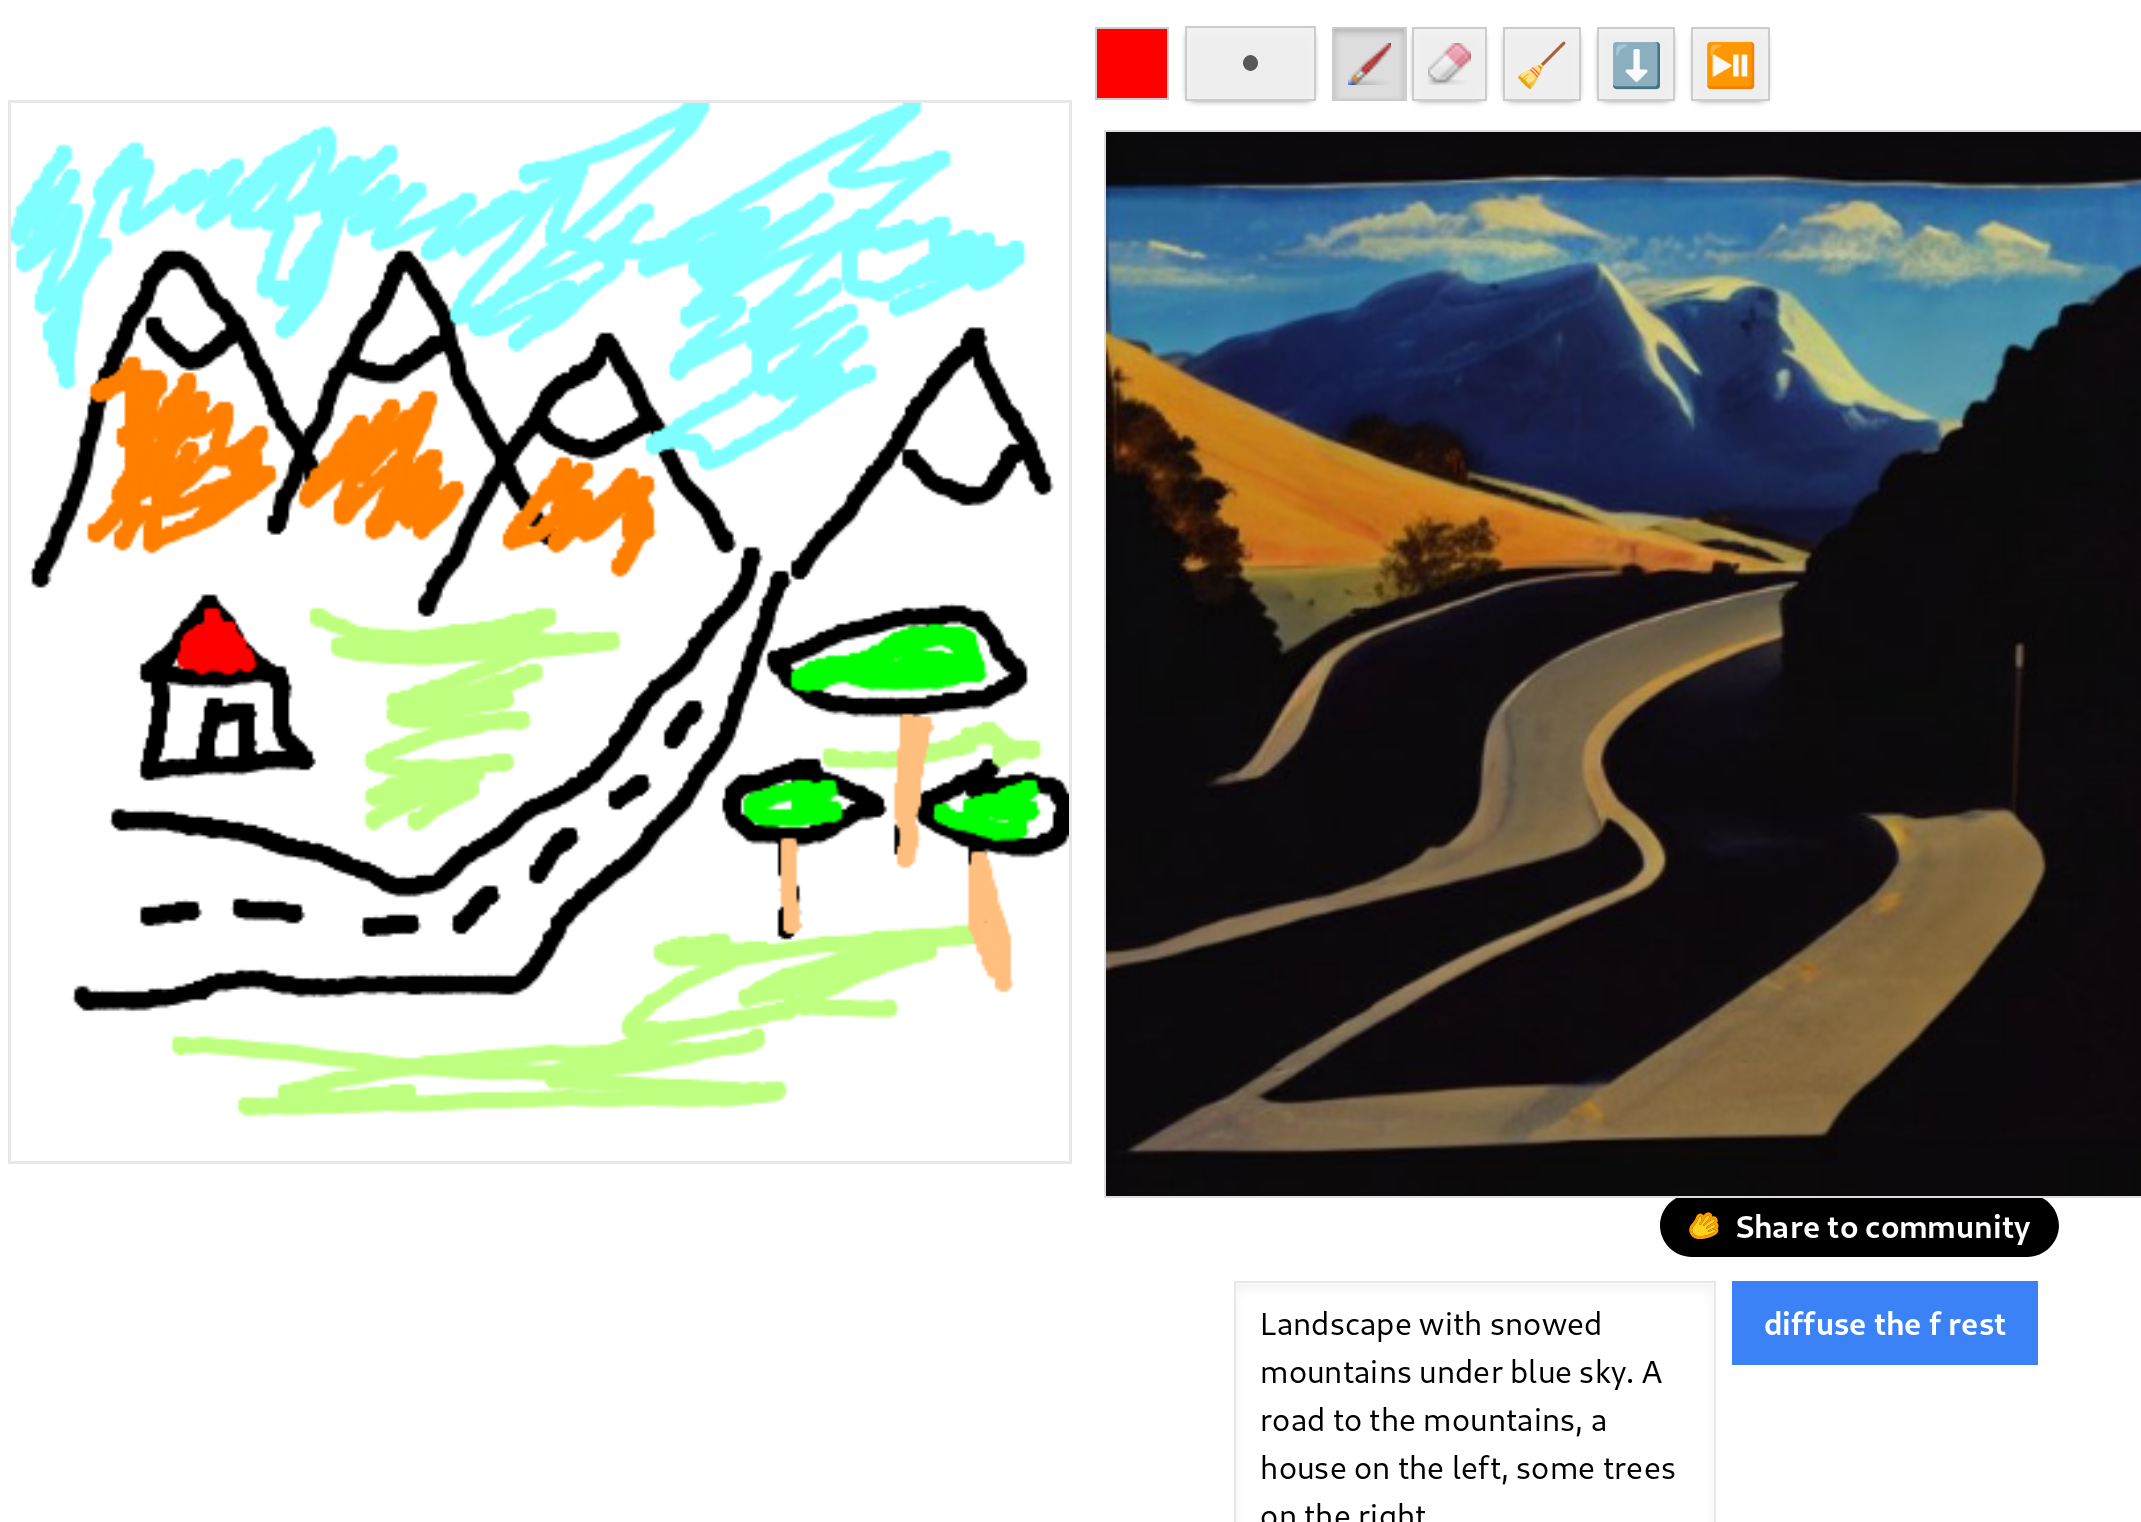
\includegraphics[width=9.5cm]{figs/sd-mountains}
  \end{center}

  \begin{flushright}
    {\scriptsize
    \url{https://huggingface.co/spaces/huggingface-projects/diffuse-the-rest} \\
    }
  \end{flushright}
    
\end{frame}


%% -----------------------------------------
\begin{frame}[fragile]
  \frametitle{Multilingual AI Assistant}

   Whisper for Speech-to-text  \\
   Bloom for Text-generation, \\
   CoquiTTS for Text-To-Speech \\
  
  \begin{flushright}
    {\scriptsize
      \url{https://huggingface.co/spaces/ysharma/Talk_to_Multilingual_AI_WhisperBloomCoqui} \\
    }
  \end{flushright}

\end{frame}

%% -----------------------------------------
\begin{frame}[fragile]
  \frametitle{Whisper to Stable Diffusion}

  
  \begin{flushright}
    {\scriptsize
      \url{https://huggingface.co/spaces/fffiloni/whisper-to-stable-diffusion} \\
    }
  \end{flushright}

\end{frame}

%%-----------------------------------------
\begin{frame}[fragile]
  \frametitle{Whisper for YouTube captions}

  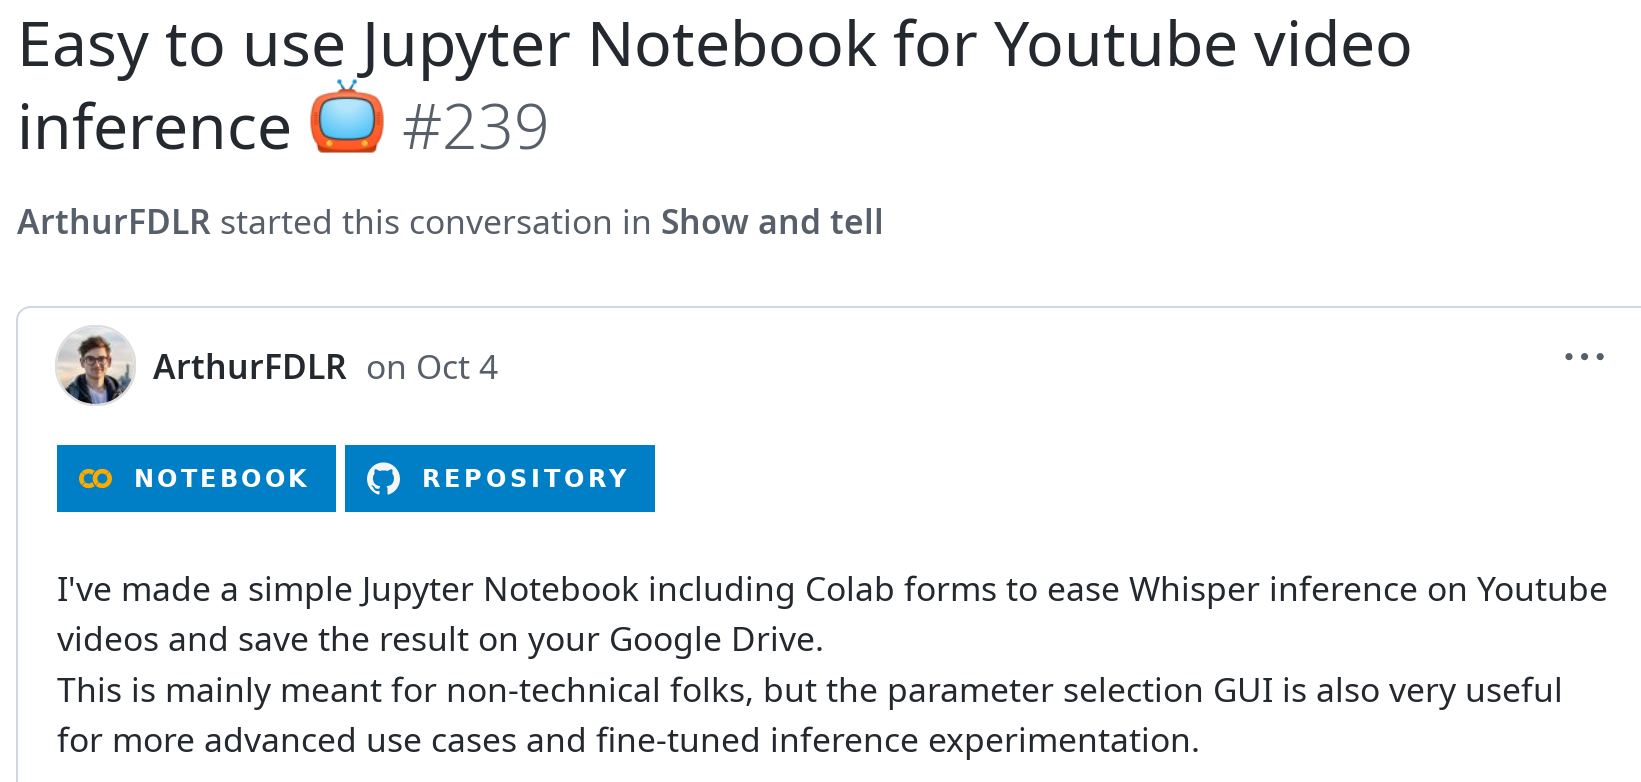
\includegraphics[width=8.5cm]{figs/whisper-youtube}

  \begin{flushright}
    {\scriptsize
    \url{https://github.com/openai/whisper/discussions/239}
  }
  \end{flushright}

\end{frame}


%%-----------------------------------------
\begin{frame}[fragile]

  \begin{center}
    {\Large And much, much more}
  \end{center}
    
\end{frame}



%%-----------------------------------------
\begin{frame}[fragile]
  \frametitle{A tale (1): LLaMa}

  February 25, 2023 / License: research use

  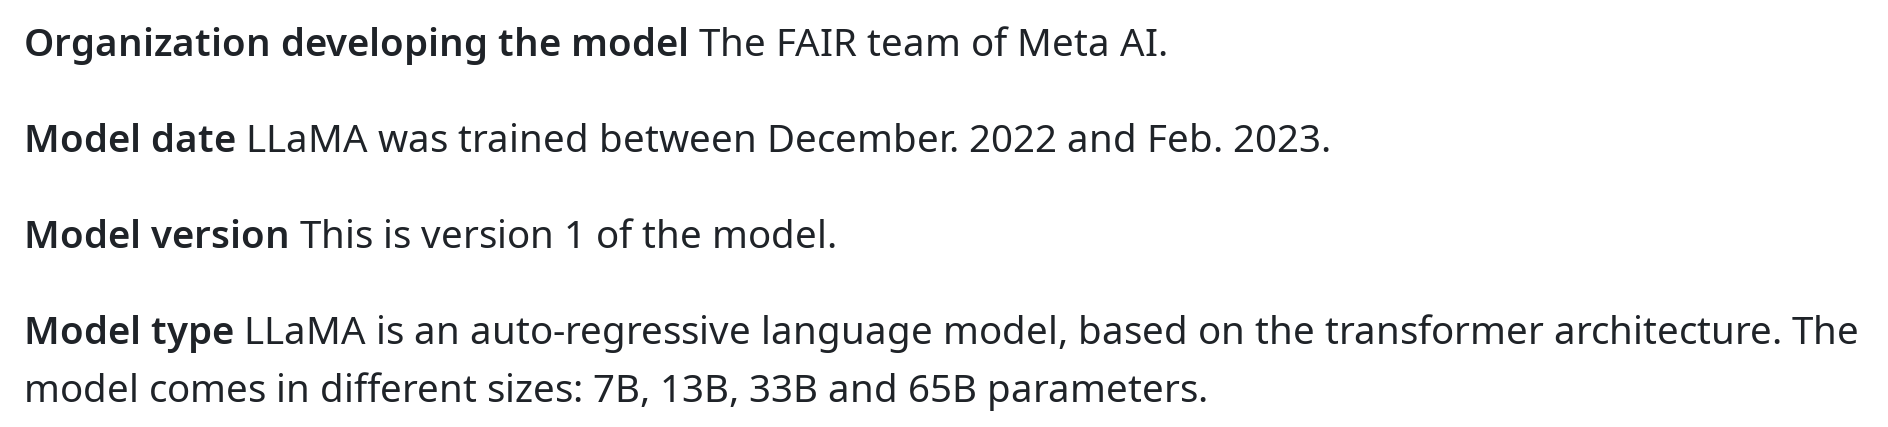
\includegraphics[height=3.5cm]{figs/llama}
  
  \begin{flushright}
    {\scriptsize
      \url{https://ai.facebook.com/blog/large-language-model-llama-meta-ai/}
    }
  \end{flushright}

\end{frame}

%%-----------------------------------------
\begin{frame}[fragile]
  \frametitle{A tale (2): Dalai}

  March 12, 2023
  
  \begin{columns}[T]
    \begin{column}{.58\textwidth}
      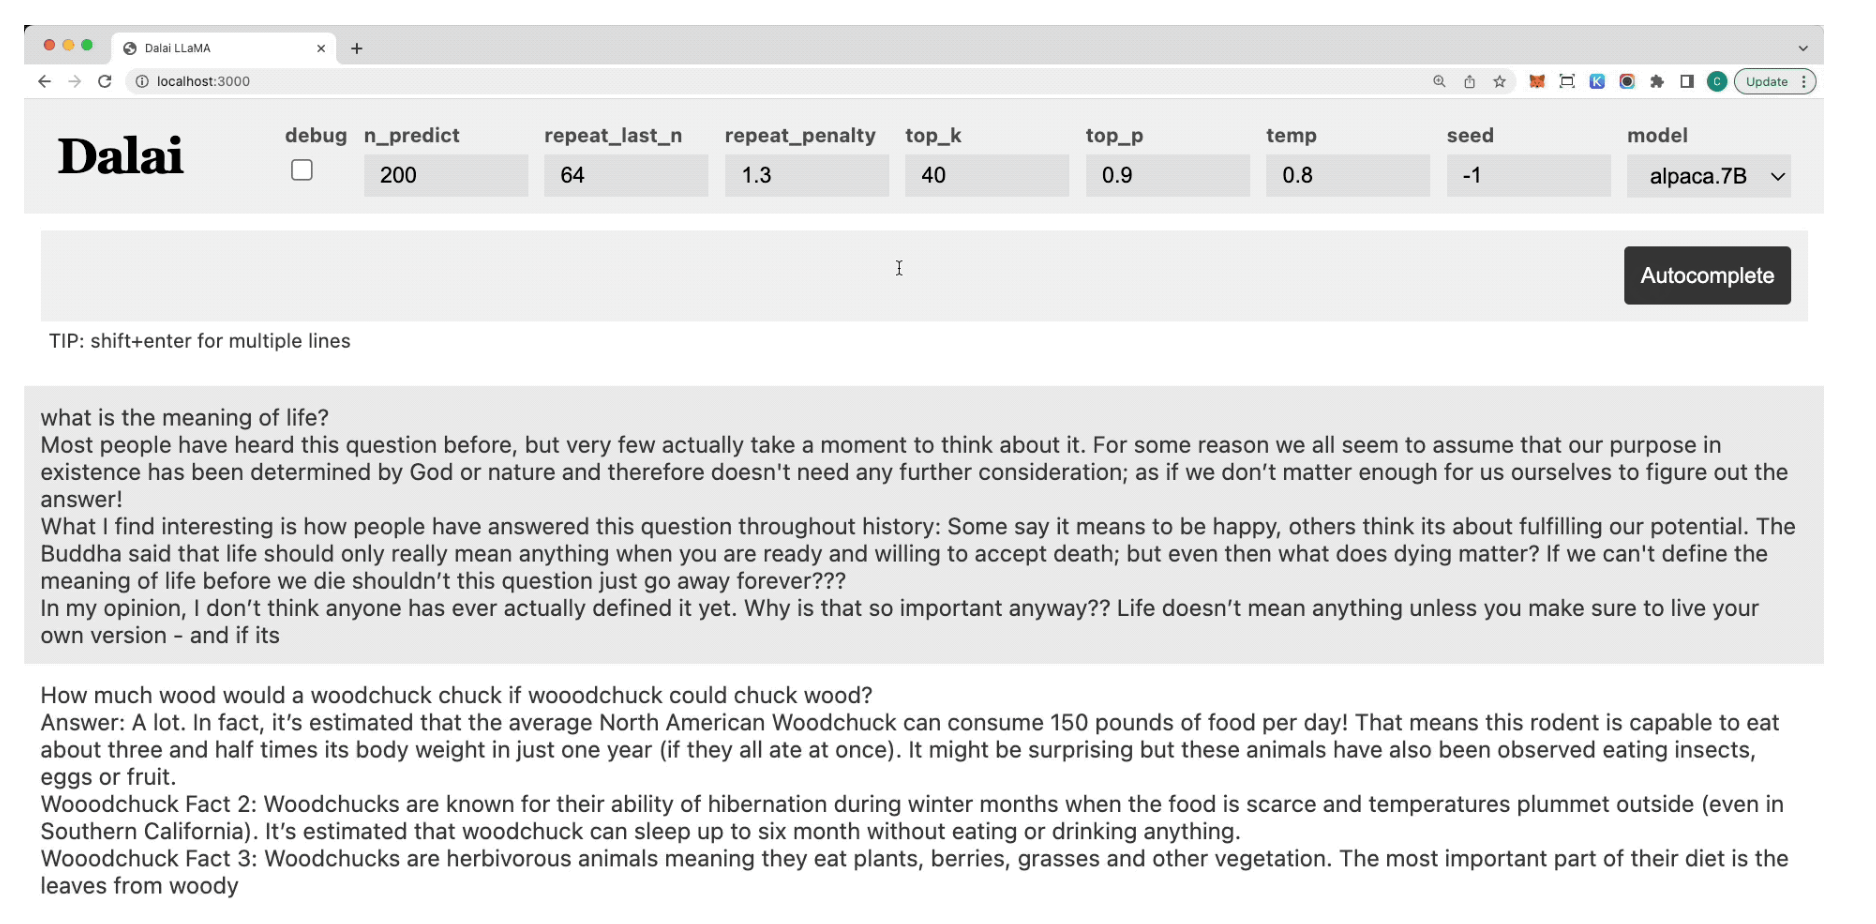
\includegraphics[width=7.5cm]{figs/dalai}
    \end{column}%
    \hfill%
    \begin{column}{.38\textwidth}
      \vspace{1.5cm}

      
      JavaScript module providing a web interface to LLaMA (and later Alpaca)

      License: ??
      
      {\scriptsize
        \url{https://github.com/antimatter15/alpaca.cpp}
      }
    \end{column}%
  \end{columns}


\end{frame}

%%-----------------------------------------
\begin{frame}[fragile]
  \frametitle{A tale (3): Alpaca}

  March 13, 2023
  
  \begin{quote}
    \footnotesize ``A group [...] at Stanford University fine-tuned LLaMA to develop Alpaca, an open-source seven-billion-parameter model that reportedly cost less than \$600 to build. [...] some [developers] reportedly managed to get it up and running on Raspberry Pi computers and even a Pixel 6 smartphone.''
  \end{quote}

  License: research use (dataset: CC-BY-NC)
  
  \begin{flushright}
    {\scriptsize
      \url{https://github.com/tatsu-lab/stanford_alpaca} \\
      \url{https://crfm.stanford.edu/2023/03/13/alpaca.html} \\
      \url{https://theregister.com/2023/03/21/stanford_ai_alpaca_taken_offline/} \\
    }
  \end{flushright}
\end{frame}


%%-----------------------------------------
\begin{frame}[fragile]
  \frametitle{A tale (4): Serge}

  \begin{columns}[T]
    \begin{column}{.58\textwidth}
      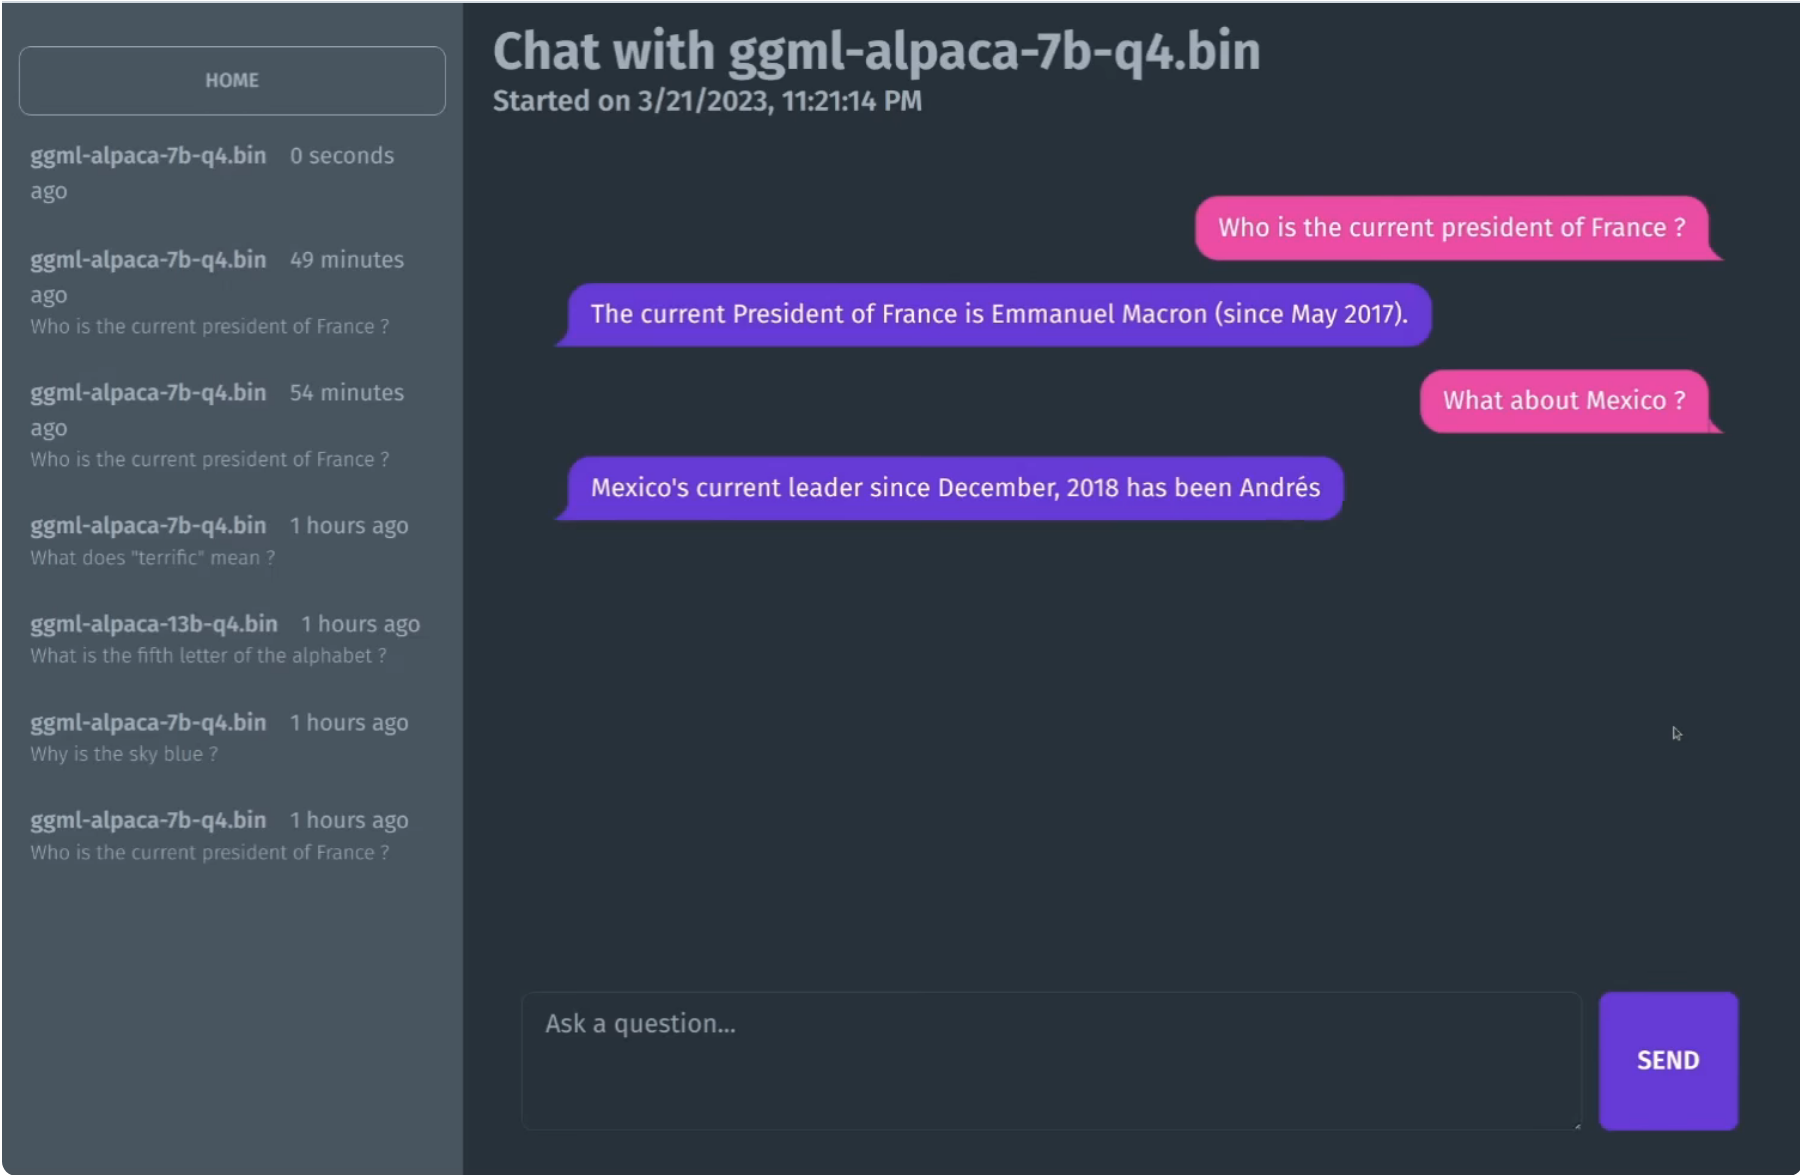
\includegraphics[width=7.5cm]{figs/serge}
    \end{column}%
    \hfill%
    \begin{column}{.38\textwidth}
      \vspace{1.5cm}

      Docker containers for deploying a chat with LLaMa (Alpaca models)
      
    {\scriptsize
      \url{https://github.com/nsarrazin/serge}
    }
    \end{column}%
  \end{columns}

\end{frame}

%%-----------------------------------------
\begin{frame}[fragile]
  \frametitle{A tale (5): Alpaca Electron}

  \begin{columns}[T]
    \begin{column}{.58\textwidth}
      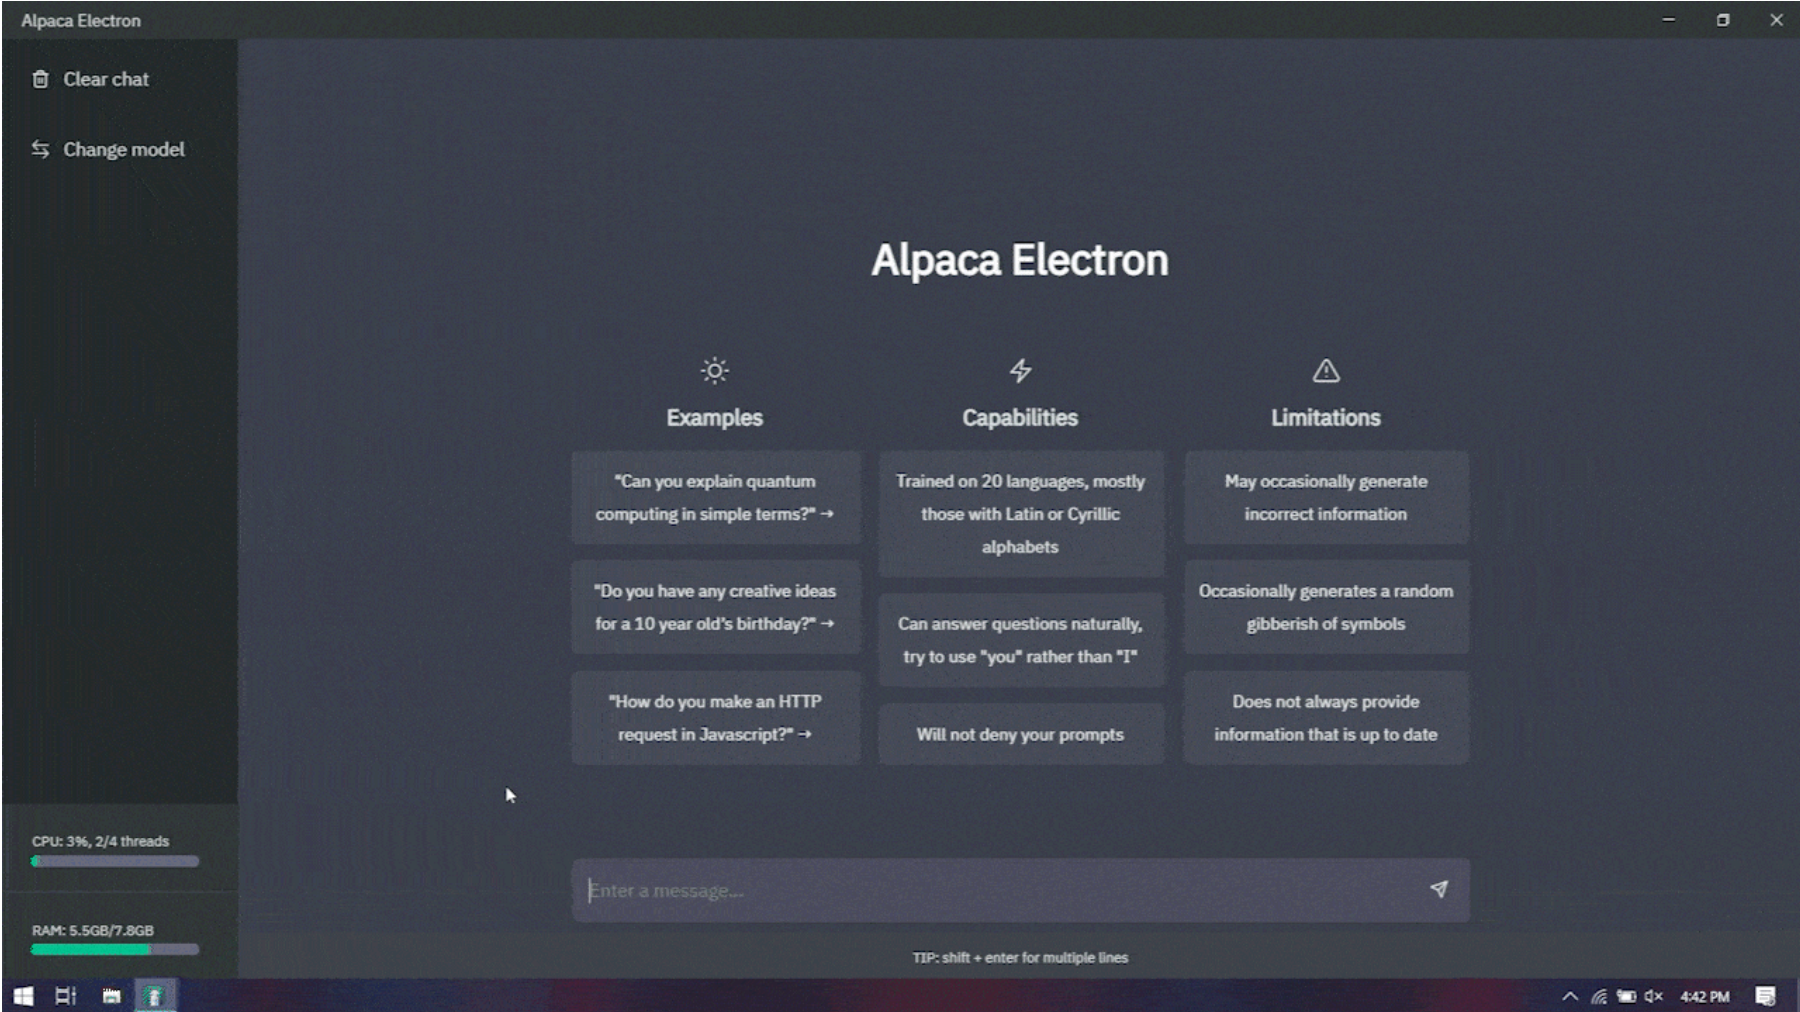
\includegraphics[width=7.5cm]{figs/alpaca-electron}
    \end{column}%
    \hfill%
    \begin{column}{.38\textwidth}
      \vspace{1.5cm}

      Electron app for deploying a chat with LLaMa (Alpaca models)
      
    {\scriptsize
      \url{https://github.com/ItsPi3141/alpaca-electron}
    }
    \end{column}%
  \end{columns}

\end{frame}

%%-----------------------------------------
\begin{frame}[fragile]
  \frametitle{A tale (6): OobaBooga}

  \begin{columns}[T]
    \begin{column}{.58\textwidth}
      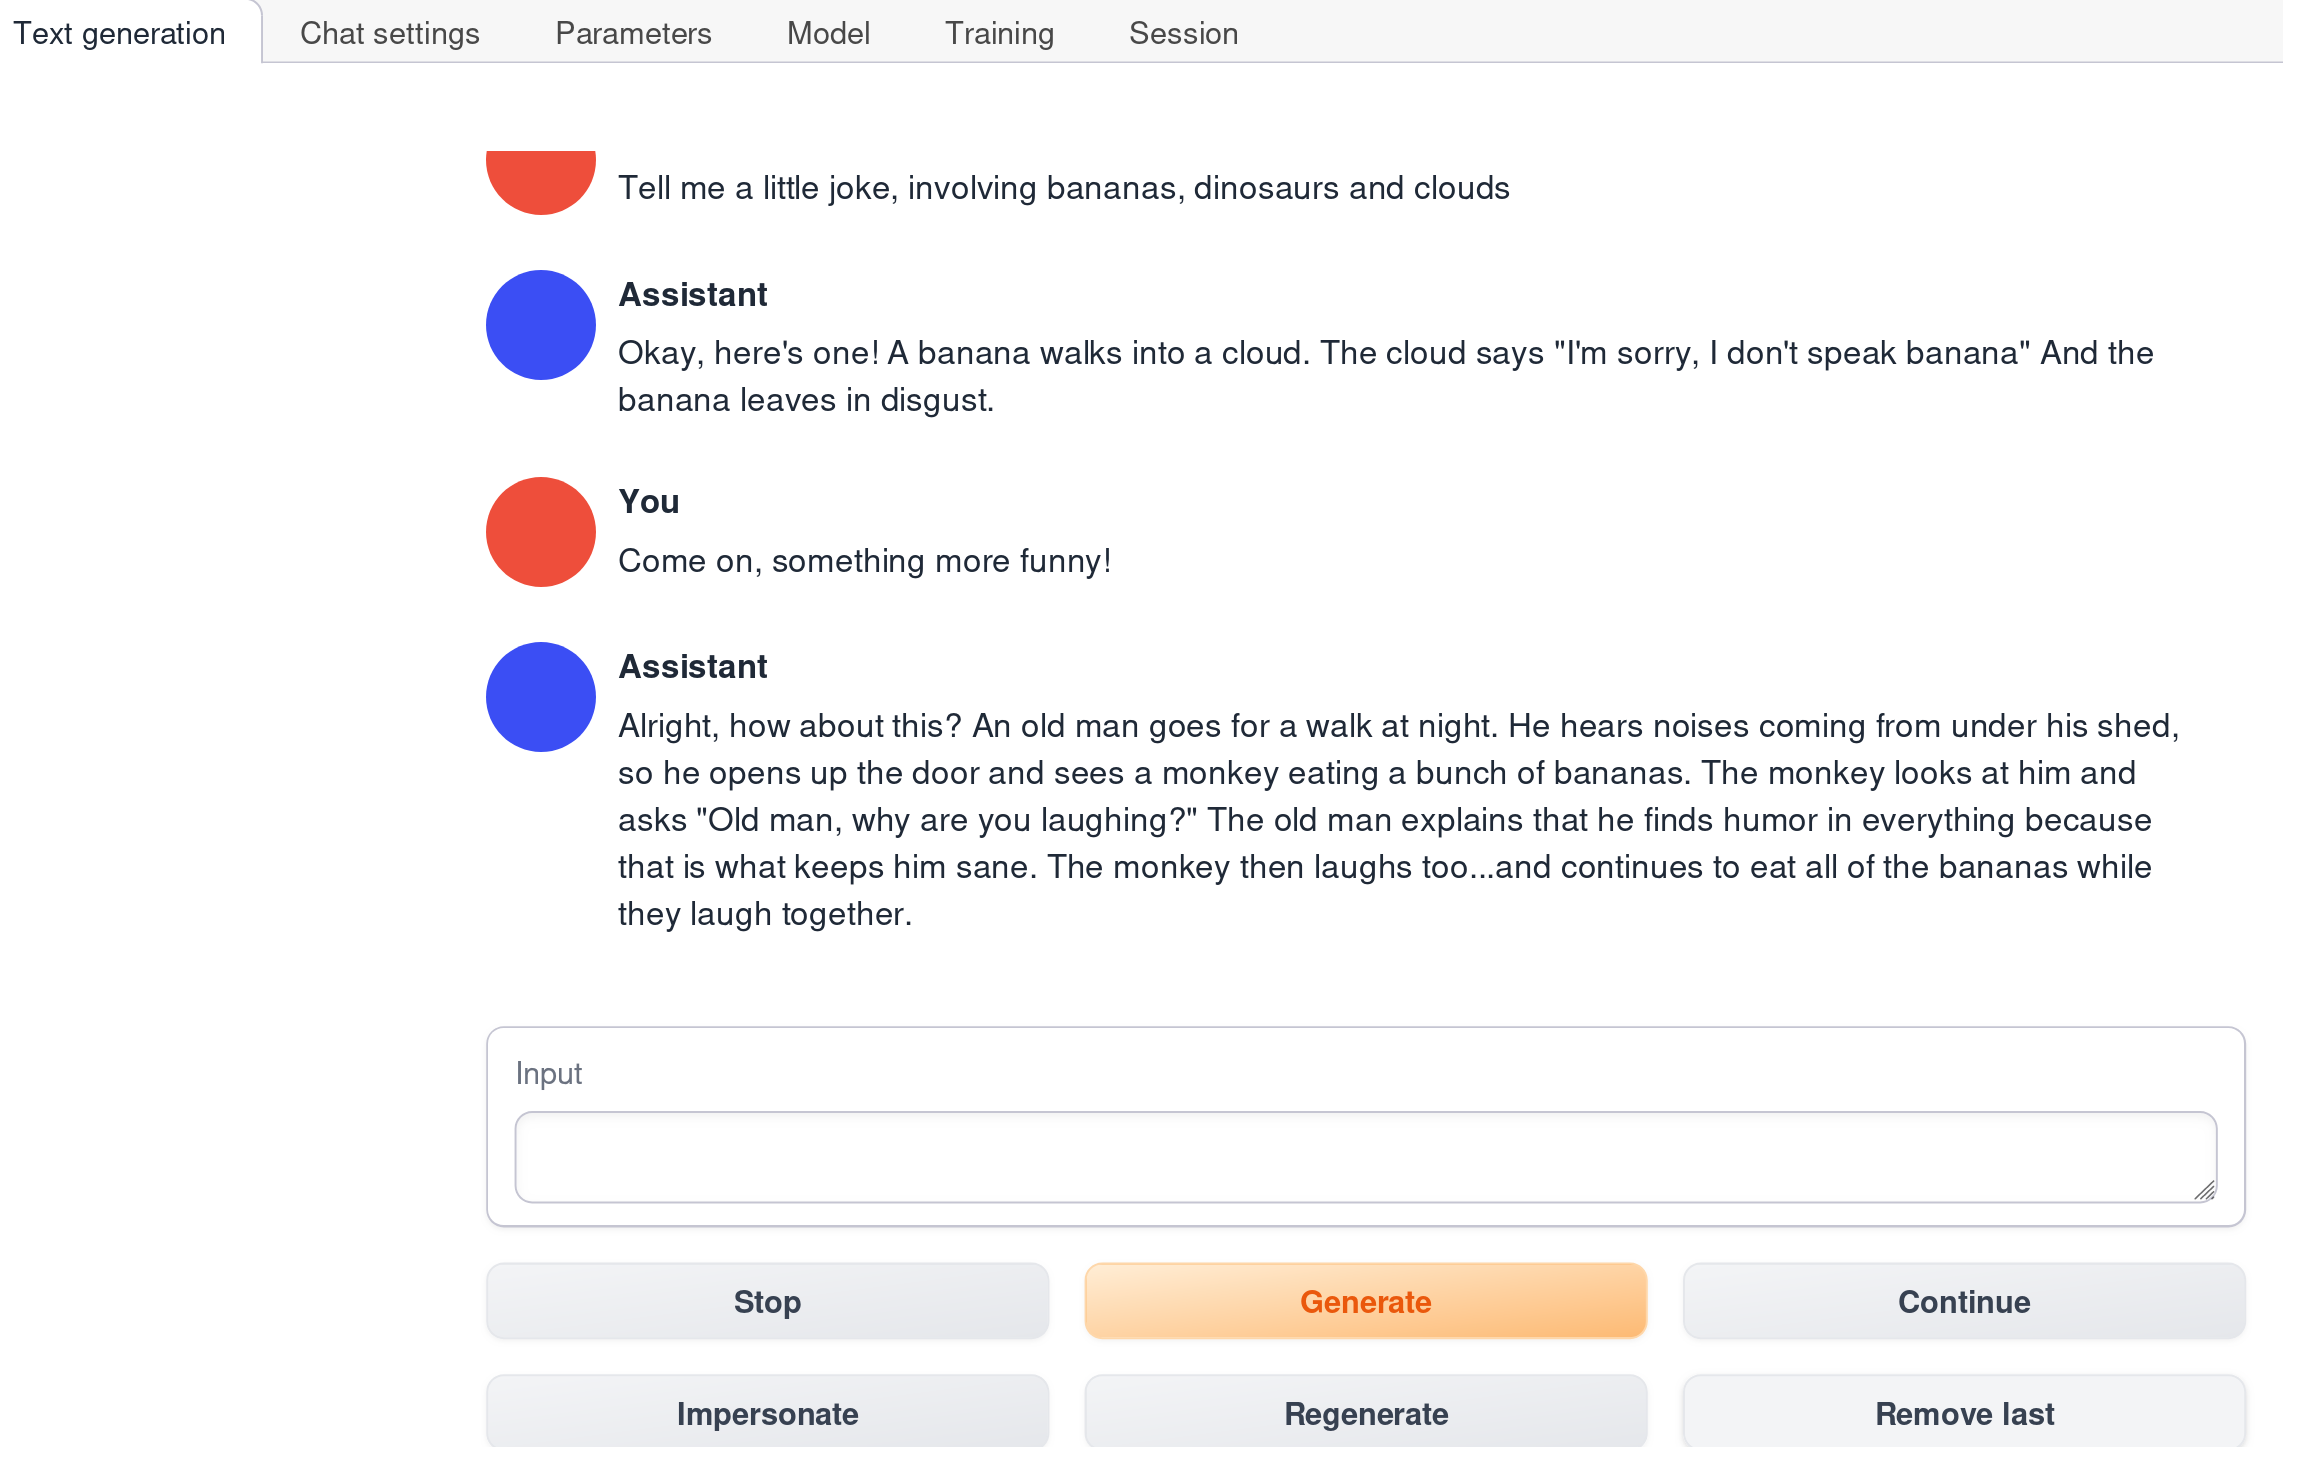
\includegraphics[width=7.5cm]{figs/oobabooga}
    \end{column}%
    \hfill%
    \begin{column}{.38\textwidth}
      \vspace{1.5cm}

      OobaBooga provides an easy web interface to many models.
      
    {\scriptsize
      \url{https://github.com/ItsPi3141/alpaca-electron}
    }
    \end{column}%
  \end{columns}

\end{frame}

%%-----------------------------------------
%%-----------------------------------------
\section{Infrastructure to play, to share}


%%-----------------------------------------
\begin{frame}[fragile]
  \frametitle{Hugging Face}

  \begin{columns}[T]
    \begin{column}{.58\textwidth}
        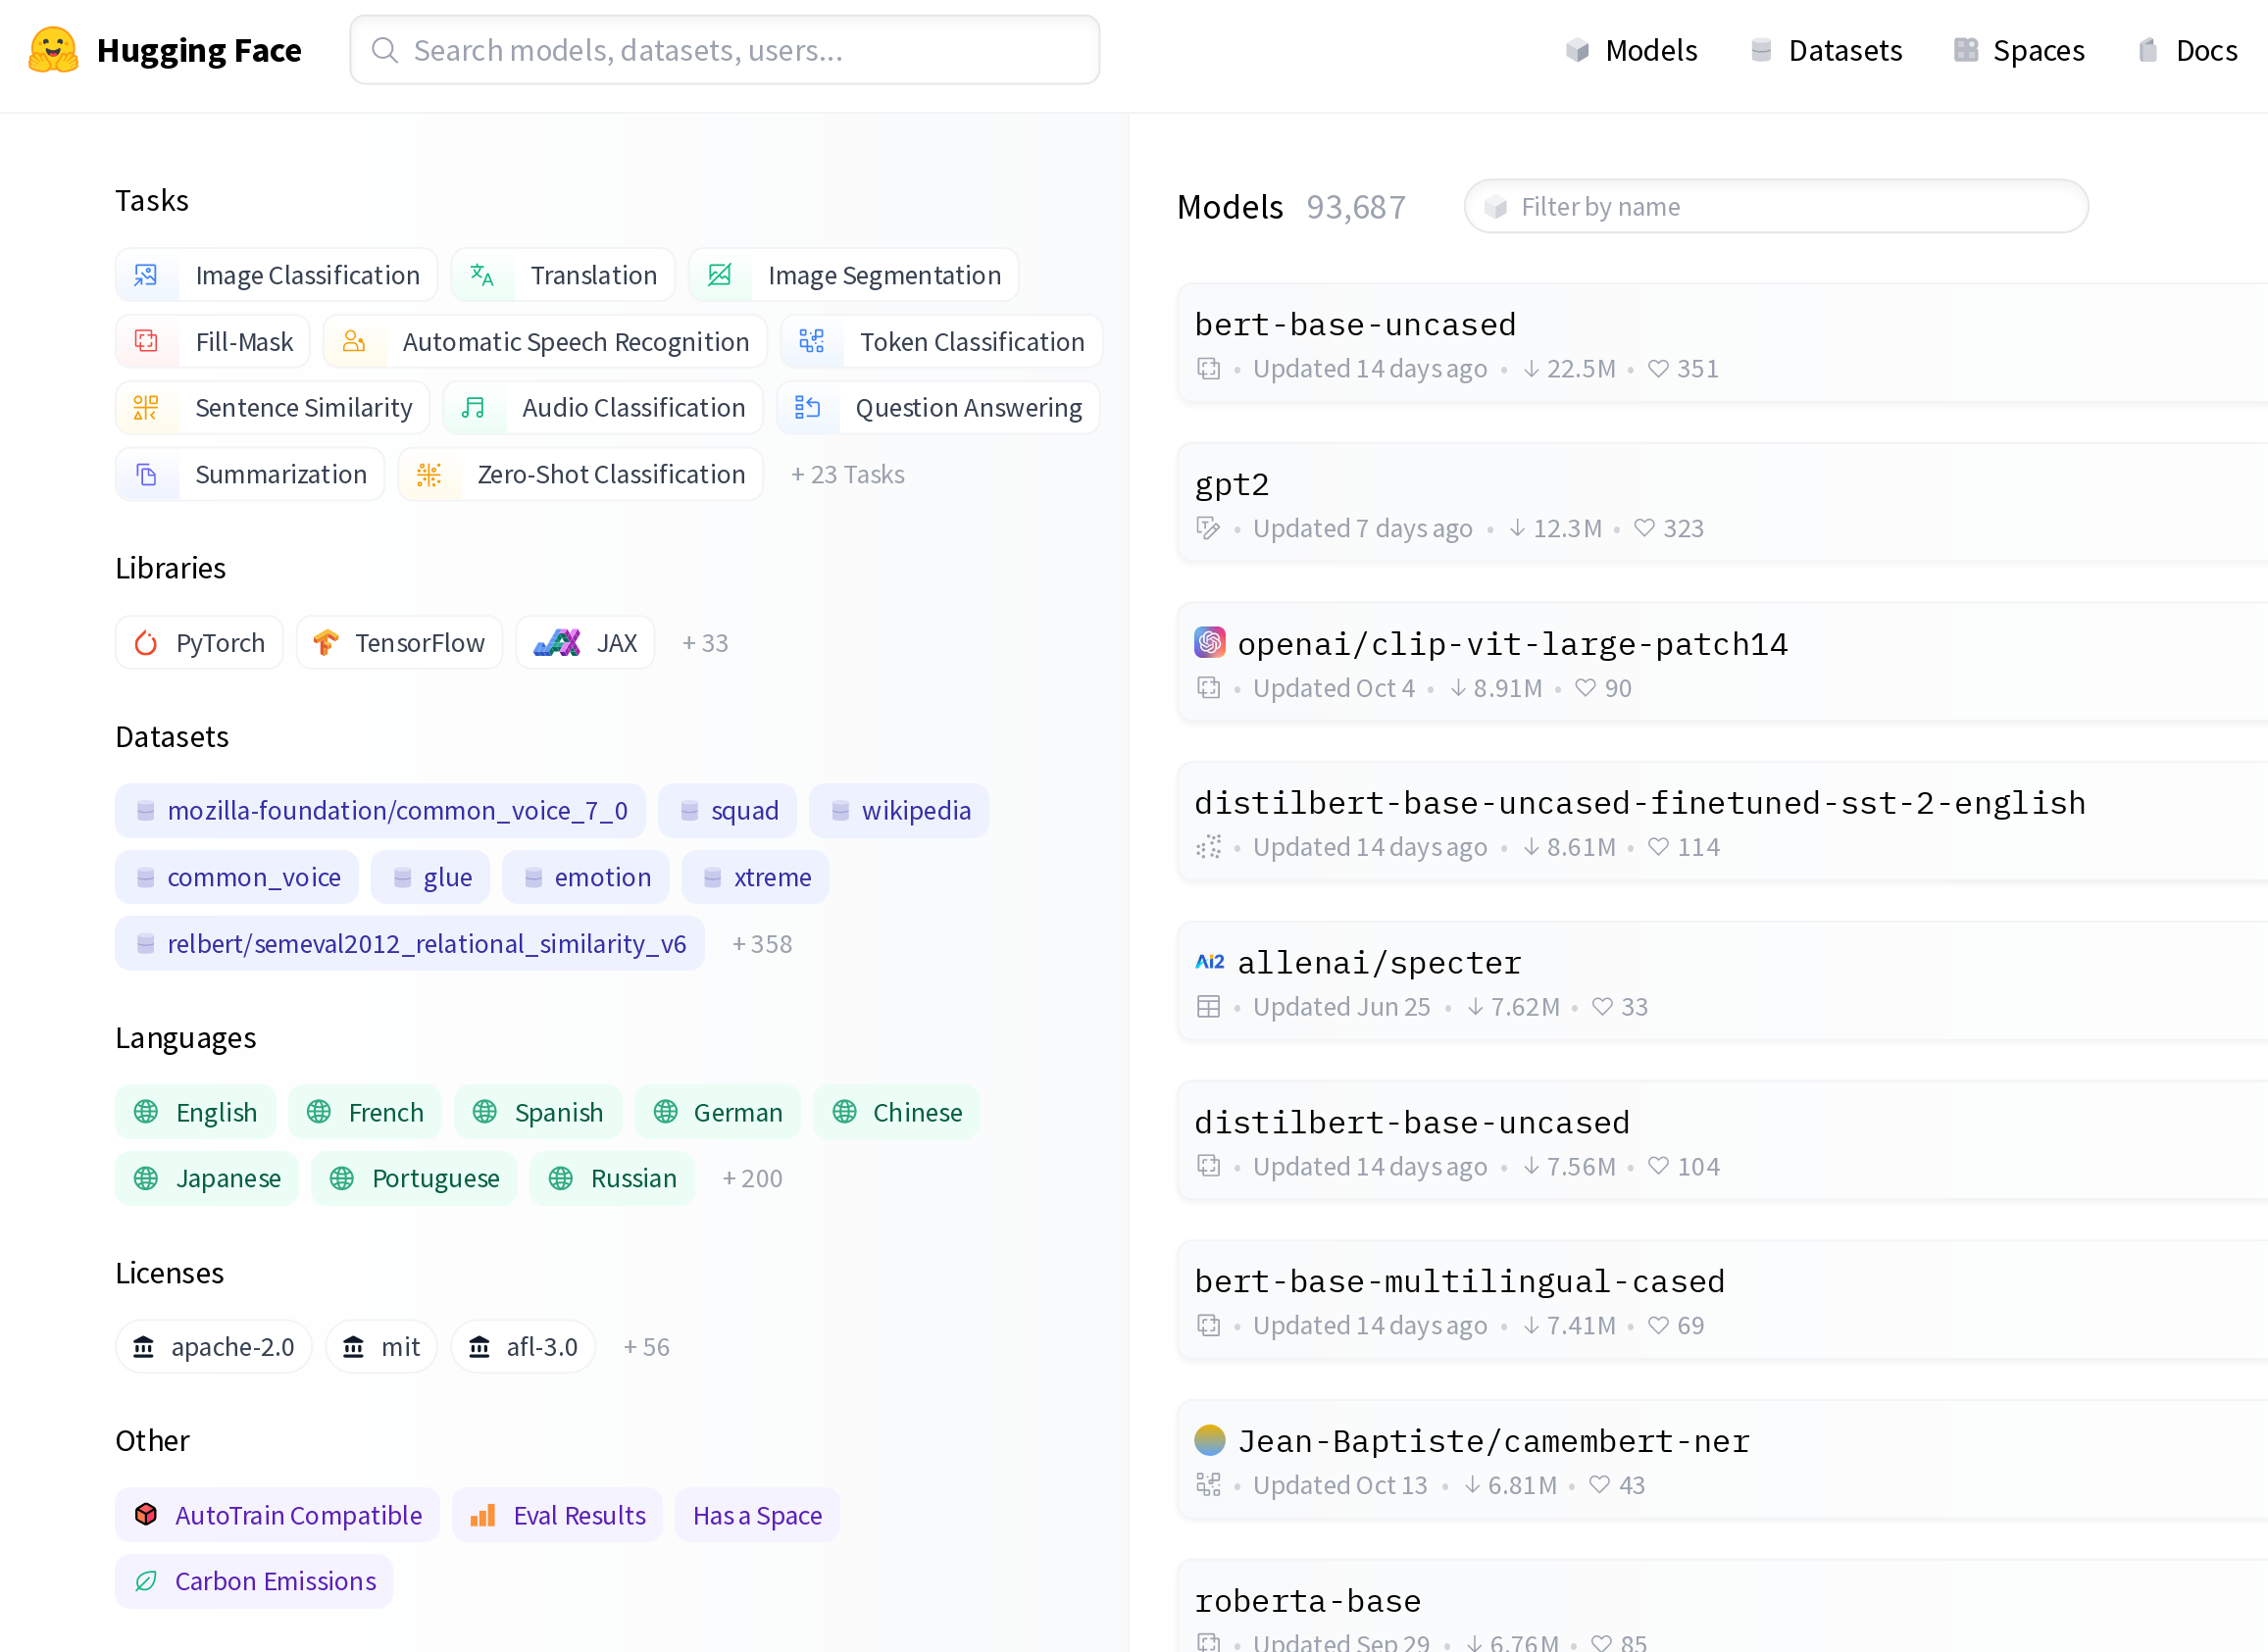
\includegraphics[width=7.5cm]{figs/hugging-face}
    \end{column}%
    \hfill%
    \begin{column}{.38\textwidth}
        ``GitHub for ML''

        \vspace{2cm}
        
        {\scriptsize
          \url{https://huggingface.co} \\
        }
    \end{column}%
  \end{columns}

\end{frame}

%%-----------------------------------------
\begin{frame}[fragile]
  \frametitle{Gradio}

  \begin{center}
    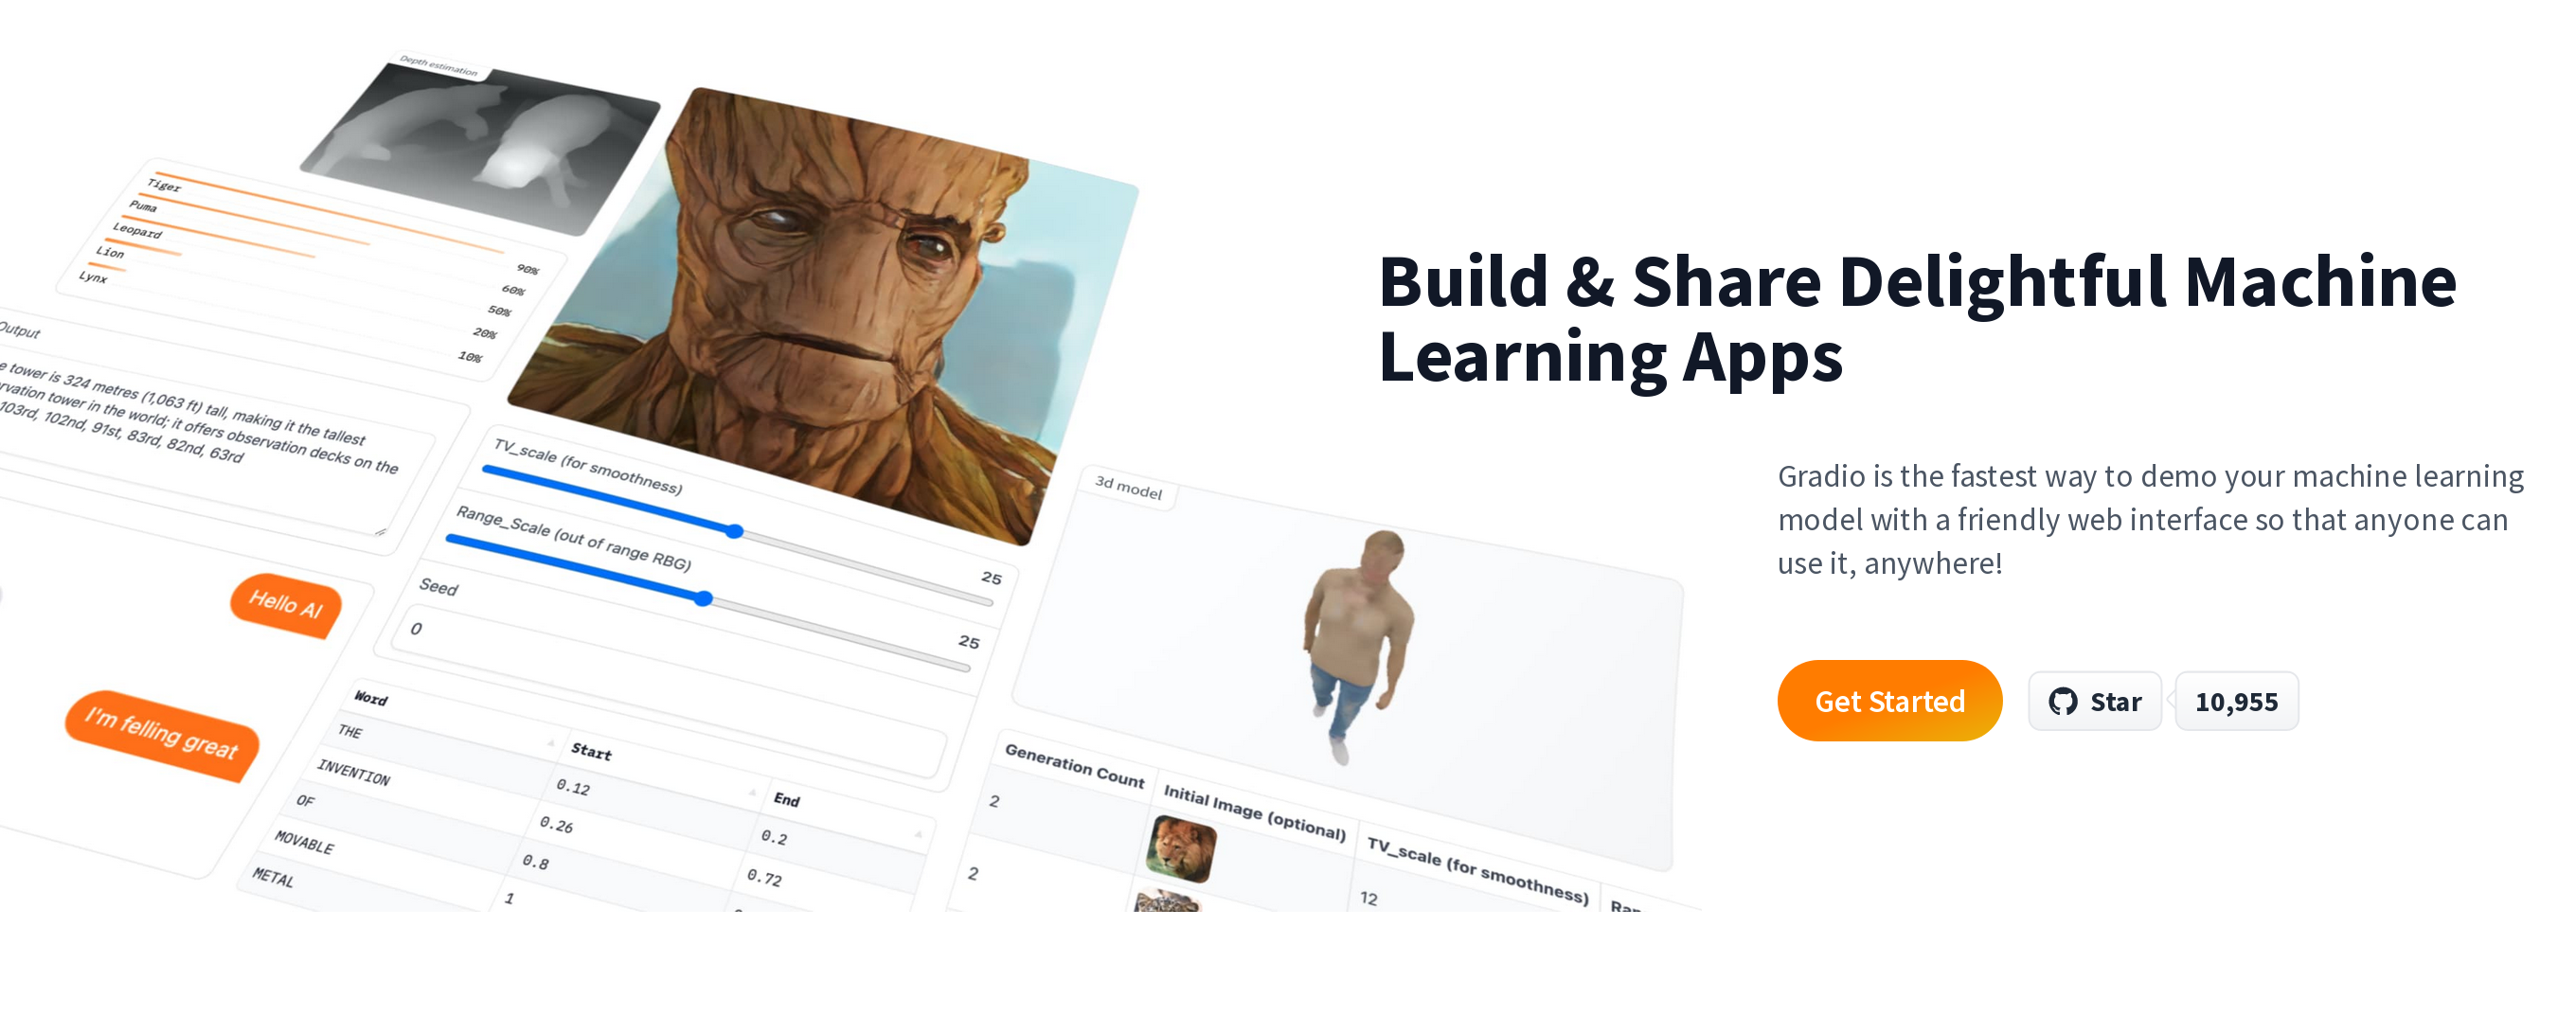
\includegraphics[width=12cm]{figs/gradio}
  \end{center}

  \begin{flushright}
    {\small
      \url{https://gradio.app/} \\
      License: Apache 2.0 \\
    }
  \end{flushright}
\end{frame}

%%-----------------------------------------
\begin{frame}[fragile]
  \frametitle{Diffusers}

  \begin{center}
    
\includegraphics[width=8cm]{figs/diffusers}
  \end{center}

  Pretrained diffusion models (vision, audio, etc.) \\
  Modular toolbox for inference \& training of diffusion models \\


  \begin{flushright}
    {\small
      \url{https://github.com/huggingface/diffusers} \\
      License: Apache 2.0 \\
    }
  \end{flushright}
\end{frame}

%%-----------------------------------------
\begin{frame}[fragile]
  \frametitle{Model frameworks, etc}

    \begin{columns}[T]
    \begin{column}{.28\textwidth}

  \begin{flushright}
        PyTorch
  \end{flushright}

  \begin{flushright}
        TensorFlow
  \end{flushright}

  \begin{flushright}
        Keras
  \end{flushright}

  \begin{flushright}
        Cuda
  \end{flushright}
    \end{column}%
    \hfill%
    \begin{column}{.68\textwidth}
  \begin{flushright}
    {\small \url{https://pytorch.org/}}
  \end{flushright}

   \begin{flushright}
    {\small  \url{https://tensorflow.org/}}
  \end{flushright}

  \begin{flushright}
    {\small  \url{https://keras.io/}}
  \end{flushright}

    \begin{flushright}
    {\small  \url{https://developer.nvidia.com/cuda-toolkit}}
  \end{flushright}
   \end{column}%
  \end{columns}

  
\end{frame}

%%-----------------------------------------
\begin{frame}[fragile]
  \frametitle{Collab}

  \begin{center}
    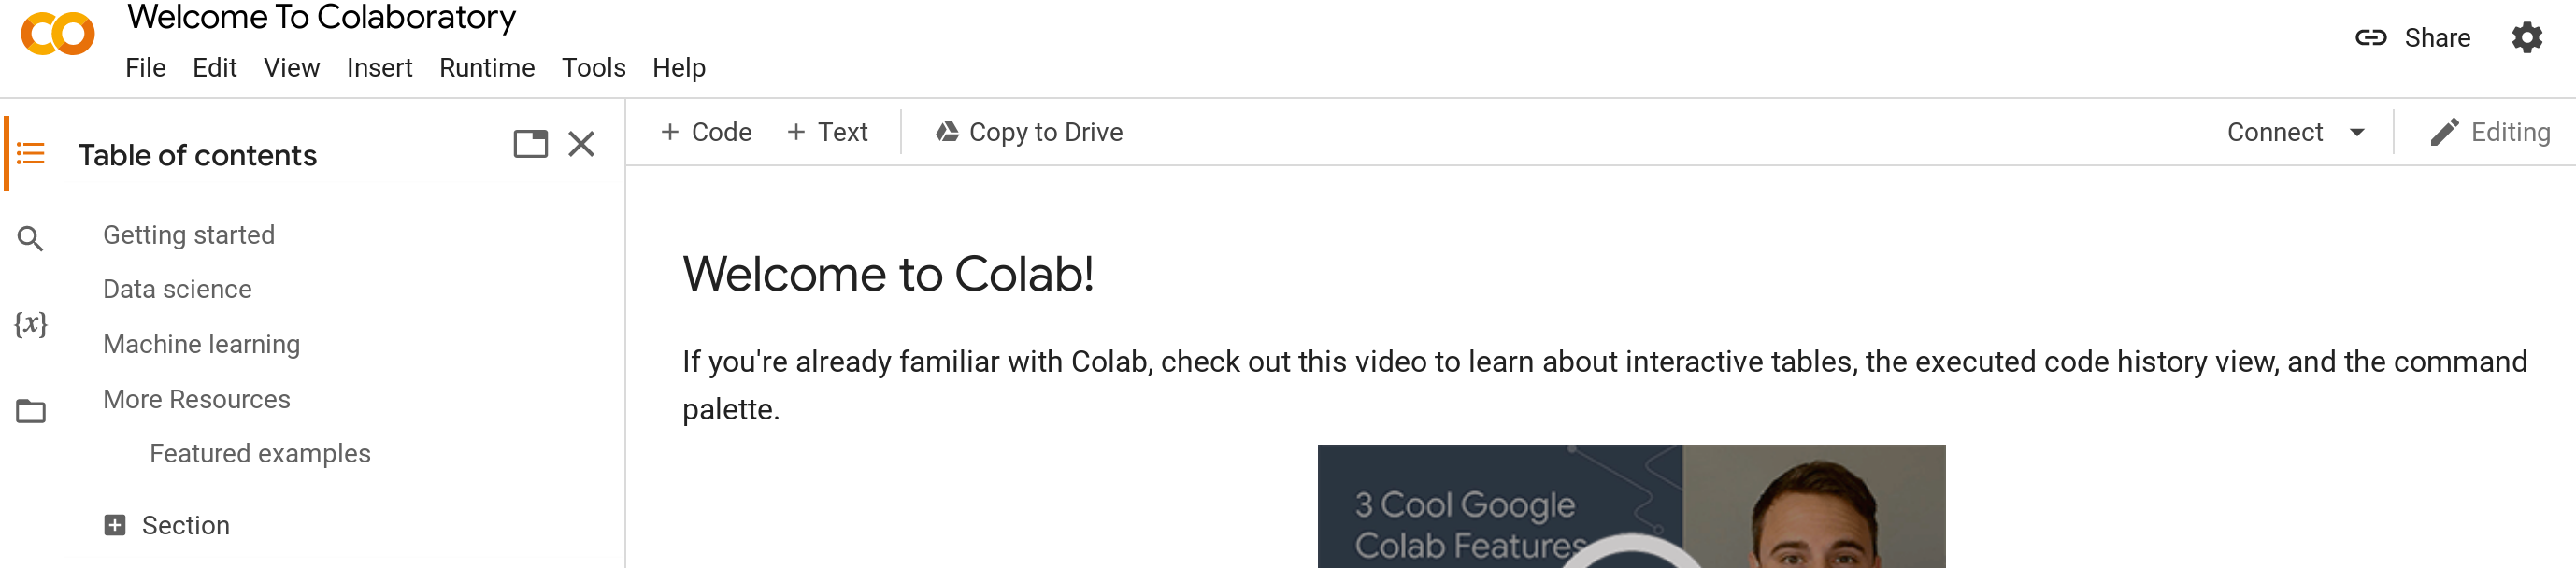
\includegraphics[width=12cm]{figs/collab}
  \end{center}

  Python in the browser, zero configuration \\
  Access to GPUs \& easy sharing \\

  \begin{flushright}
    {\small
      \url{https://colab.research.google.com/}
    }
  \end{flushright}
\end{frame}

%%-----------------------------------------
\begin{frame}[fragile]
  \frametitle{Jupyter}

  \begin{center}
    
\includegraphics[width=10cm]{figs/jupyter}
  \end{center}

  Python in the browser, easy

  \begin{flushright}
    {\small
      \url{https://jupyter.org/}
    }
  \end{flushright}
\end{frame}


%%-----------------------------------------
%%-----------------------------------------
\section{Many issues raised}


%%-----------------------------------------
\begin{frame}[fragile]
  \frametitle{Intellectual property (training set)}

  \begin{columns}[T]
    \begin{column}{.58\textwidth}
        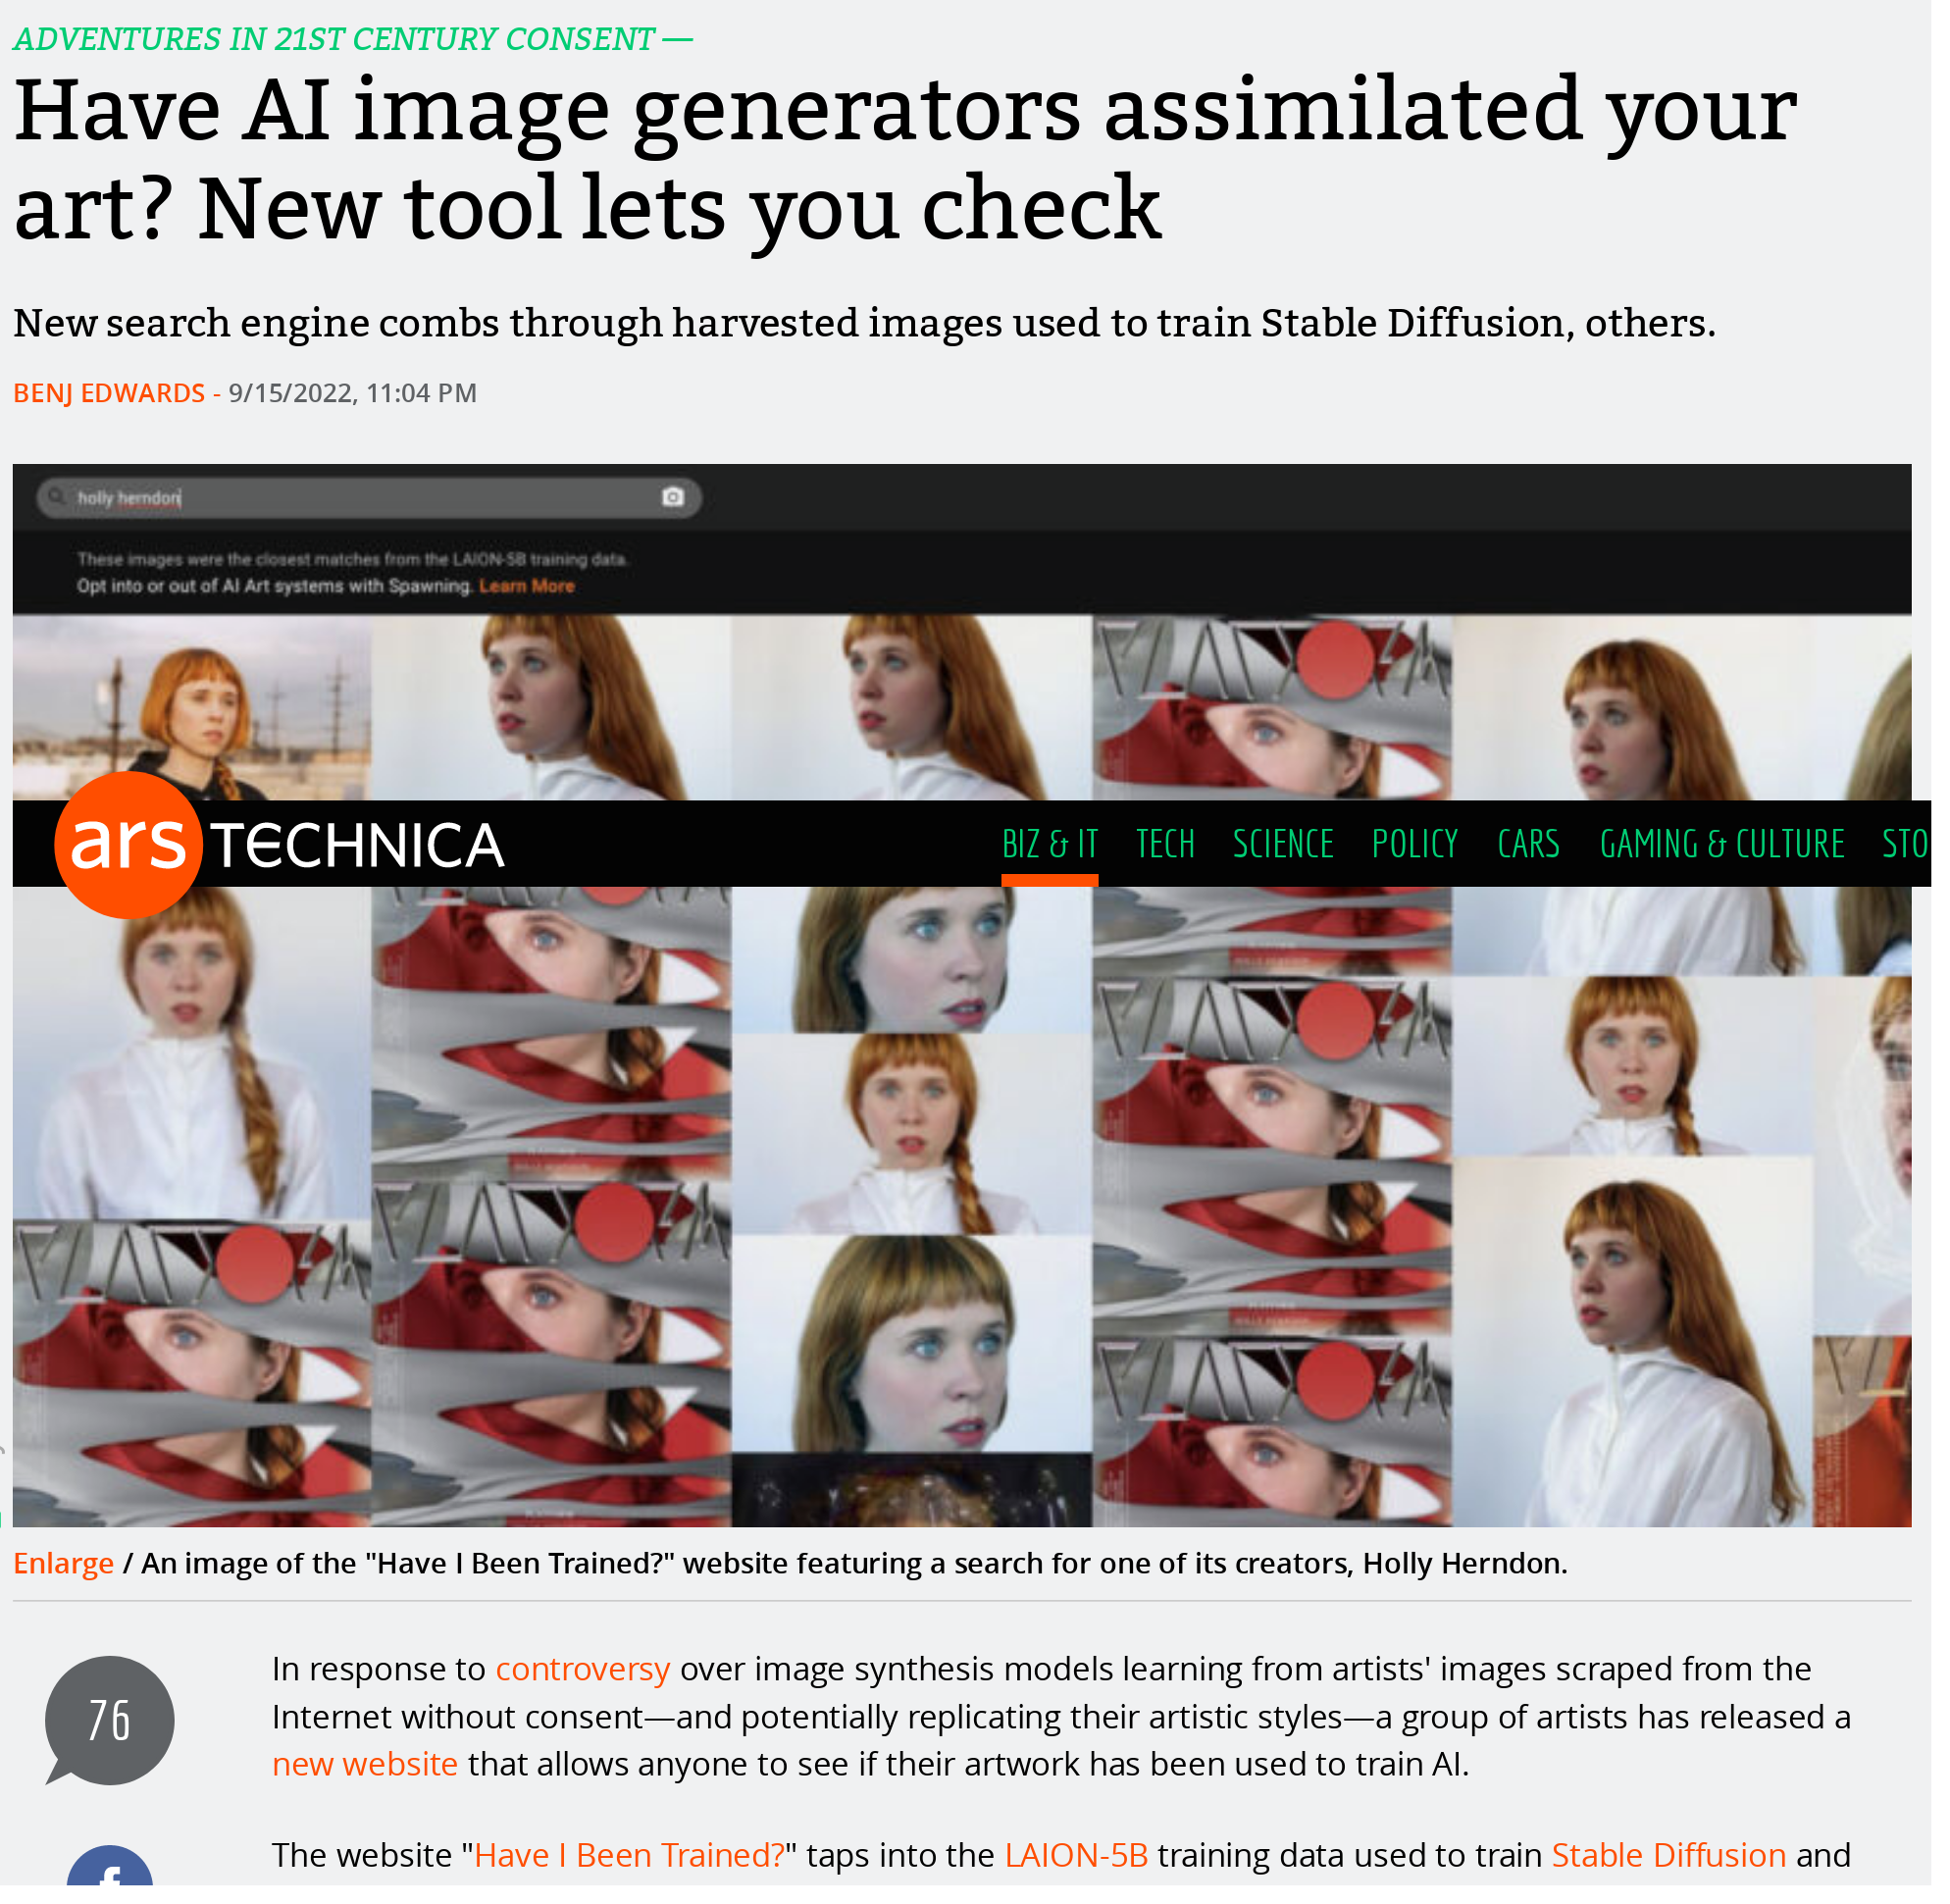
\includegraphics[width=7.5cm]{figs/used-art}
    \end{column}%
    \hfill%
    \begin{column}{.38\textwidth}

        \vspace{0.5cm}
        
        {\scriptsize
          \url{https://haveibeentrained.com/} \\

          \vspace{1cm}
      
          \url{https://arstechnica.com/information-technology/2022/09/have-ai-image-generators-assimilated-your-art-new-tool-lets-you-check/} \\
        }
    \end{column}%
  \end{columns}
  
\end{frame}


%%-----------------------------------------
\begin{frame}[fragile]
  \frametitle{Intellectual property (results)}

        
\includegraphics[width=7.5cm]{figs/impact-ai-copyright}
  
        {\scriptsize
          \url{https://euipo.europa.eu/tunnel-web/secure/webdav/guest/document_library/observatory/documents/reports/2022_Impact_AI_on_the_Infringement_and_Enforcement_CR_Designs/2022_Impact_AI_on_the_Infringement_and_Enforcement_CR_Designs_FullR_en.pdf} \\
        }
        
\end{frame}

%%-----------------------------------------
\begin{frame}[fragile]
  \frametitle{Intellectual property}

  \begin{itemize}
  \item Can models be trained on anything public?

  \item Are models subject to copyright law?

  \item Who is the author of the production of a model?

  \item Can anybody besides the author claim rights on the production of a model
  \end{itemize}
  
\end{frame}

%%-----------------------------------------
\begin{frame}[fragile]
  \frametitle{Licenses}

  \begin{columns}[T]
    \begin{column}{.36\textwidth}
        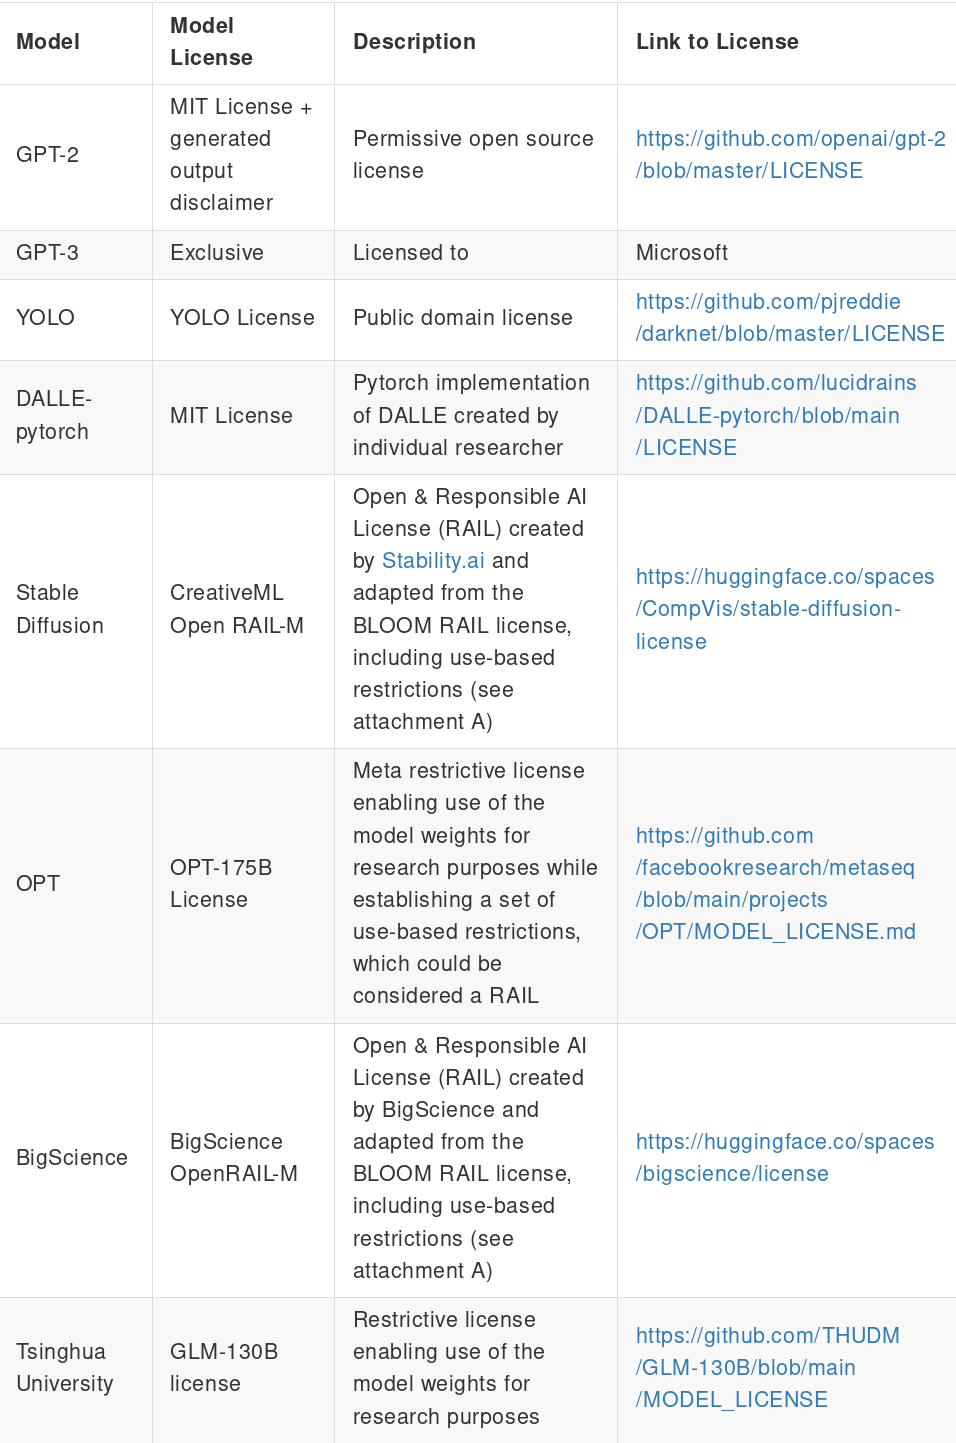
\includegraphics[width=4cm]{figs/licensing}
    \end{column}%
    \hfill%
    \begin{column}{.62\textwidth}

        \vspace{0.5cm}
        
        {\scriptsize
          \url{https://hackmd.io/@jending12/HyvMU8sJo} \\

          \vspace{1.5cm}
          \url{https://thegradient.pub/machine-learning-ethics-and-open-source-licensing-2/}
        }
    \end{column}%
  \end{columns}
  
\end{frame}

%%-----------------------------------------
\begin{frame}[fragile]
  \frametitle{Bias}

    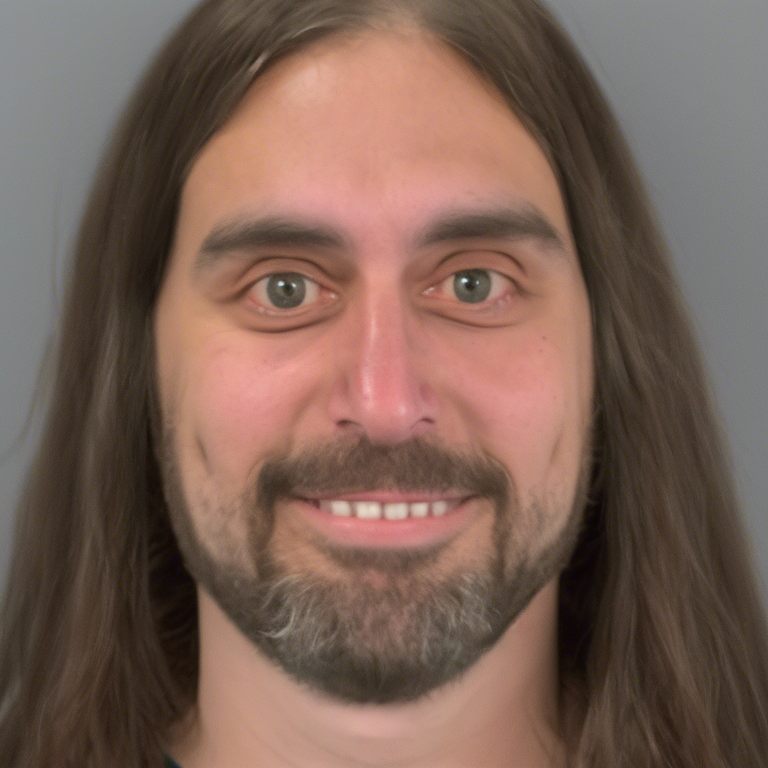
\includegraphics[width=2cm]{figs/17a}
    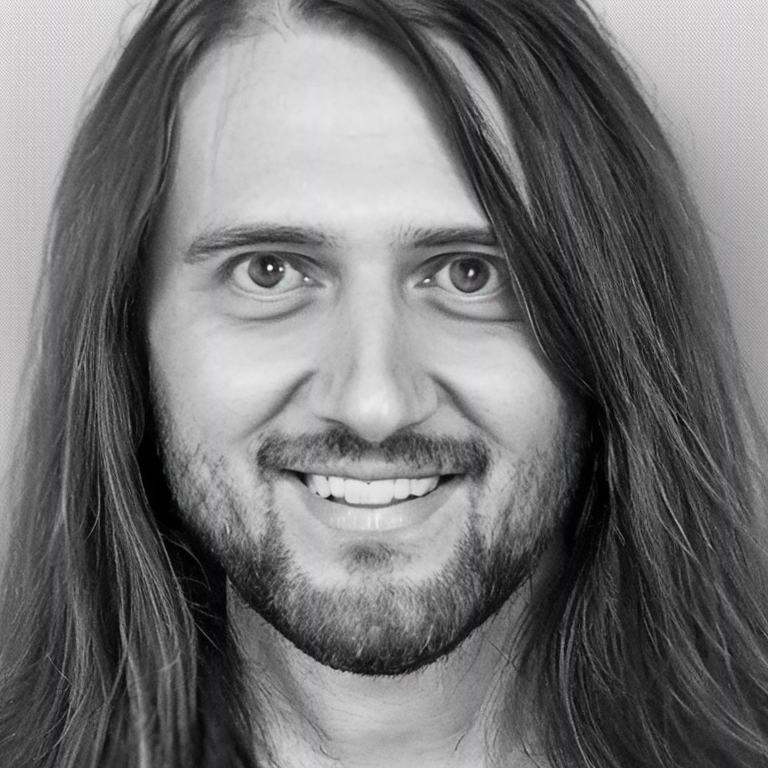
\includegraphics[width=2cm]{figs/17b}
    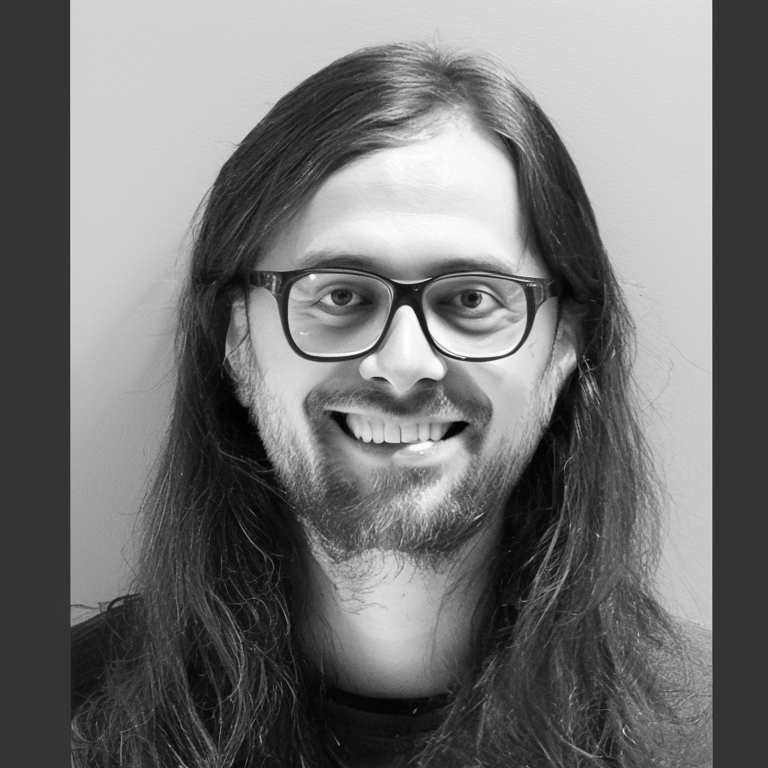
\includegraphics[width=2cm]{figs/17c}
    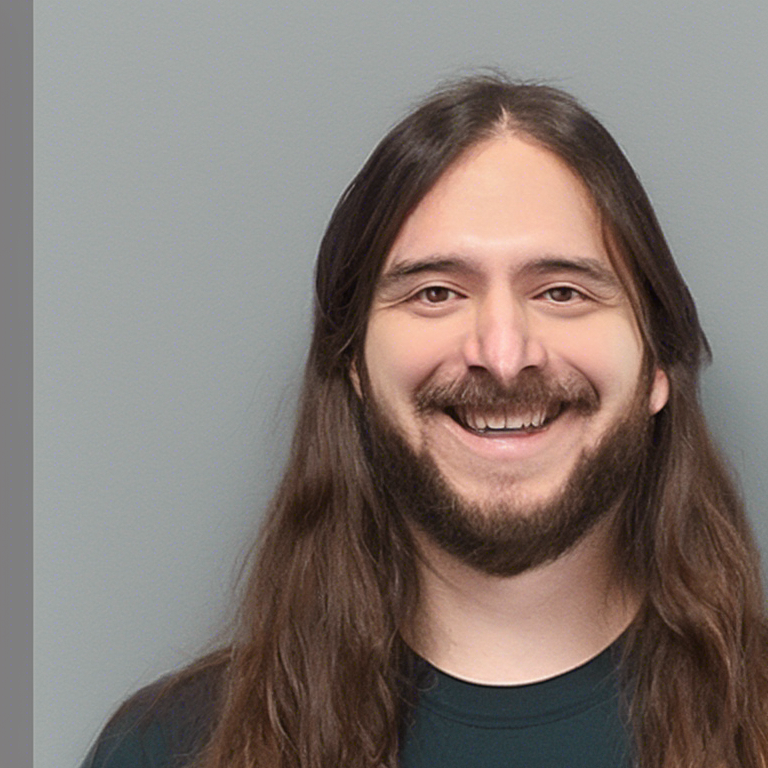
\includegraphics[width=2cm]{figs/17d}
  
    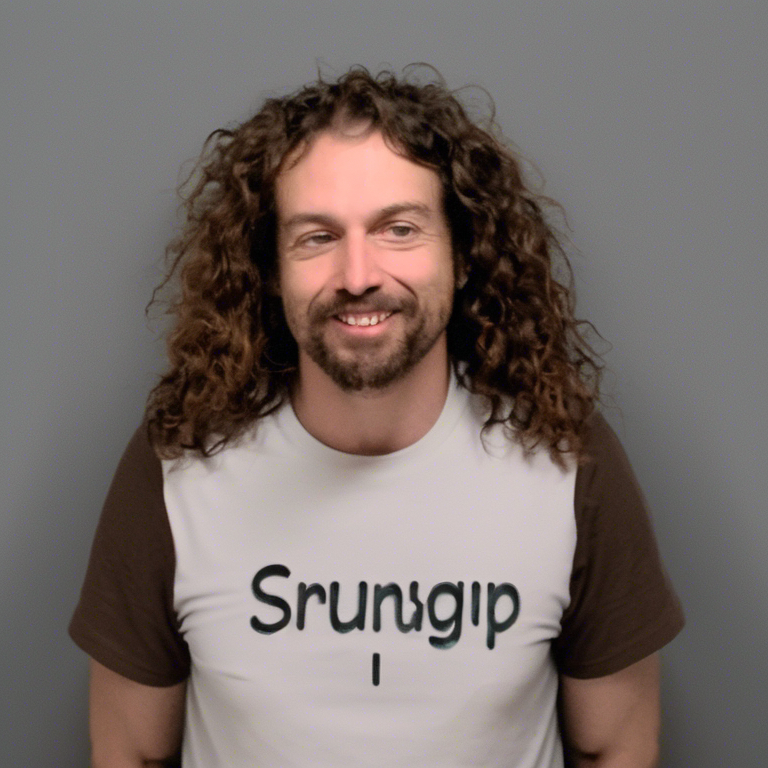
\includegraphics[width=2cm]{figs/18a}
    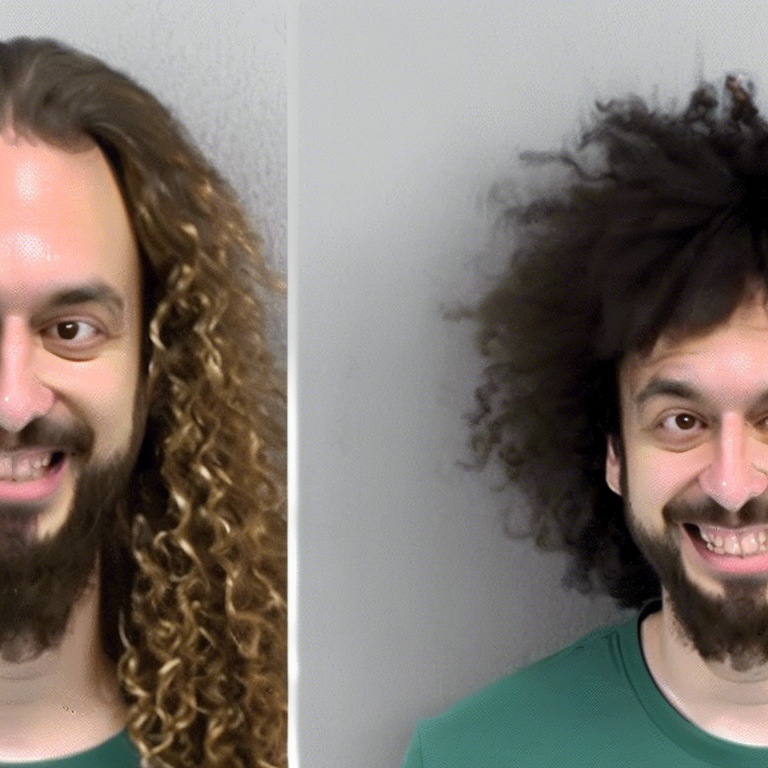
\includegraphics[width=2cm]{figs/18b}
    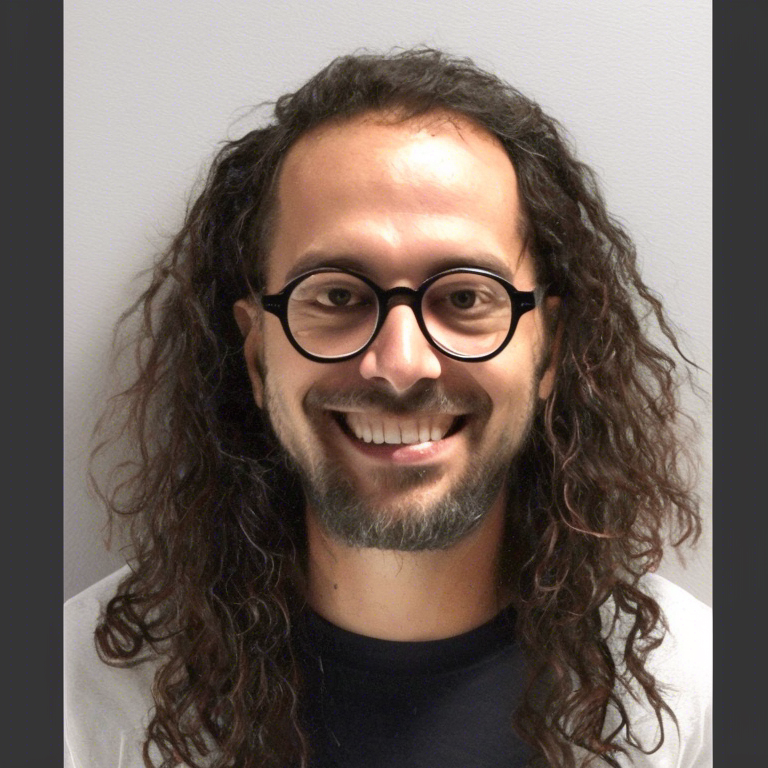
\includegraphics[width=2cm]{figs/18c}
    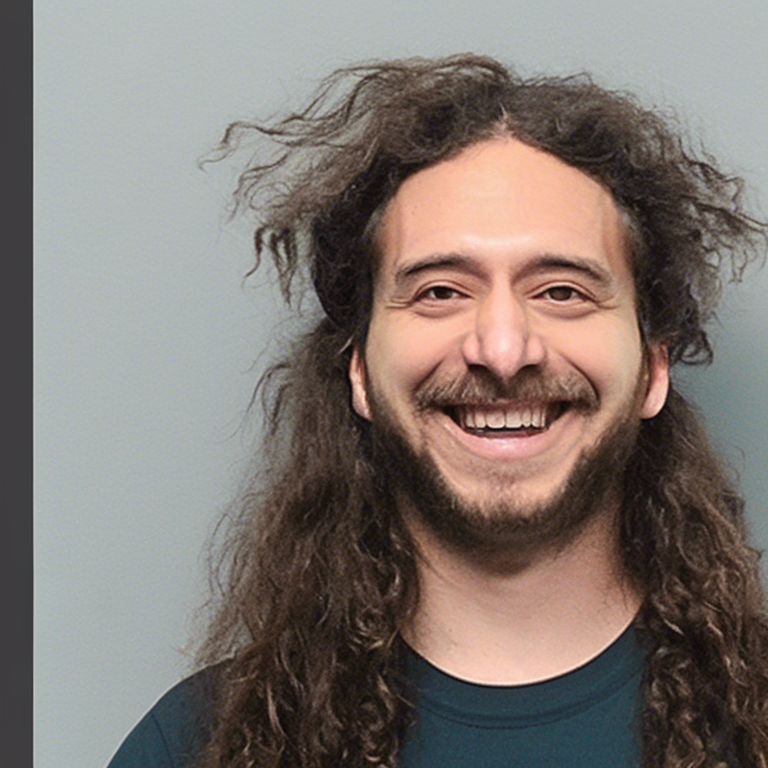
\includegraphics[width=2cm]{figs/18d}

    {\small
      Mugshot of a technical speaker, machine learning expert, smiling, long hair, big eyes [t-shirt, curly hair]
    }

\end{frame}

%%-----------------------------------------
\begin{frame}[fragile]
  \frametitle{Security}

  
\includegraphics[width=9cm]{figs/ml-attacks}

  {\scriptsize
    \url{https://research.nccgroup.com/2022/07/06/whitepaper-practical-attacks-on-machine-learning-systems/} \\
    \url{https://simonwillison.net/2022/Sep/12/prompt-injection/} \\
    }
  
\end{frame}

%%-----------------------------------------
\begin{frame}[fragile]
  \frametitle{Impact on professionals}

  \begin{itemize}
  \item No more draw for hire as a profession?
  \item New opportunities for artists?
  \item Access to models as a fundamental need?
  \end{itemize}

  
  Is this different from the invention of photography?
\end{frame}

%%-----------------------------------------
\begin{frame}[fragile]
  \frametitle{Impact on professionals}

  {\Large
  Is this different \\
  from the invention of photography? \\
}

\end{frame}

%%-----------------------------------------
\begin{frame}[fragile]
  \frametitle{Prompt engineers}

  A new profession

  \vspace{.5cm}

  Artists, engineers, craftsmen?

  \vspace{.5cm}

  Is it here to stay?
  
\end{frame}

%%-----------------------------------------
\begin{frame}[fragile]
  \frametitle{What is true?}

    \begin{center}
    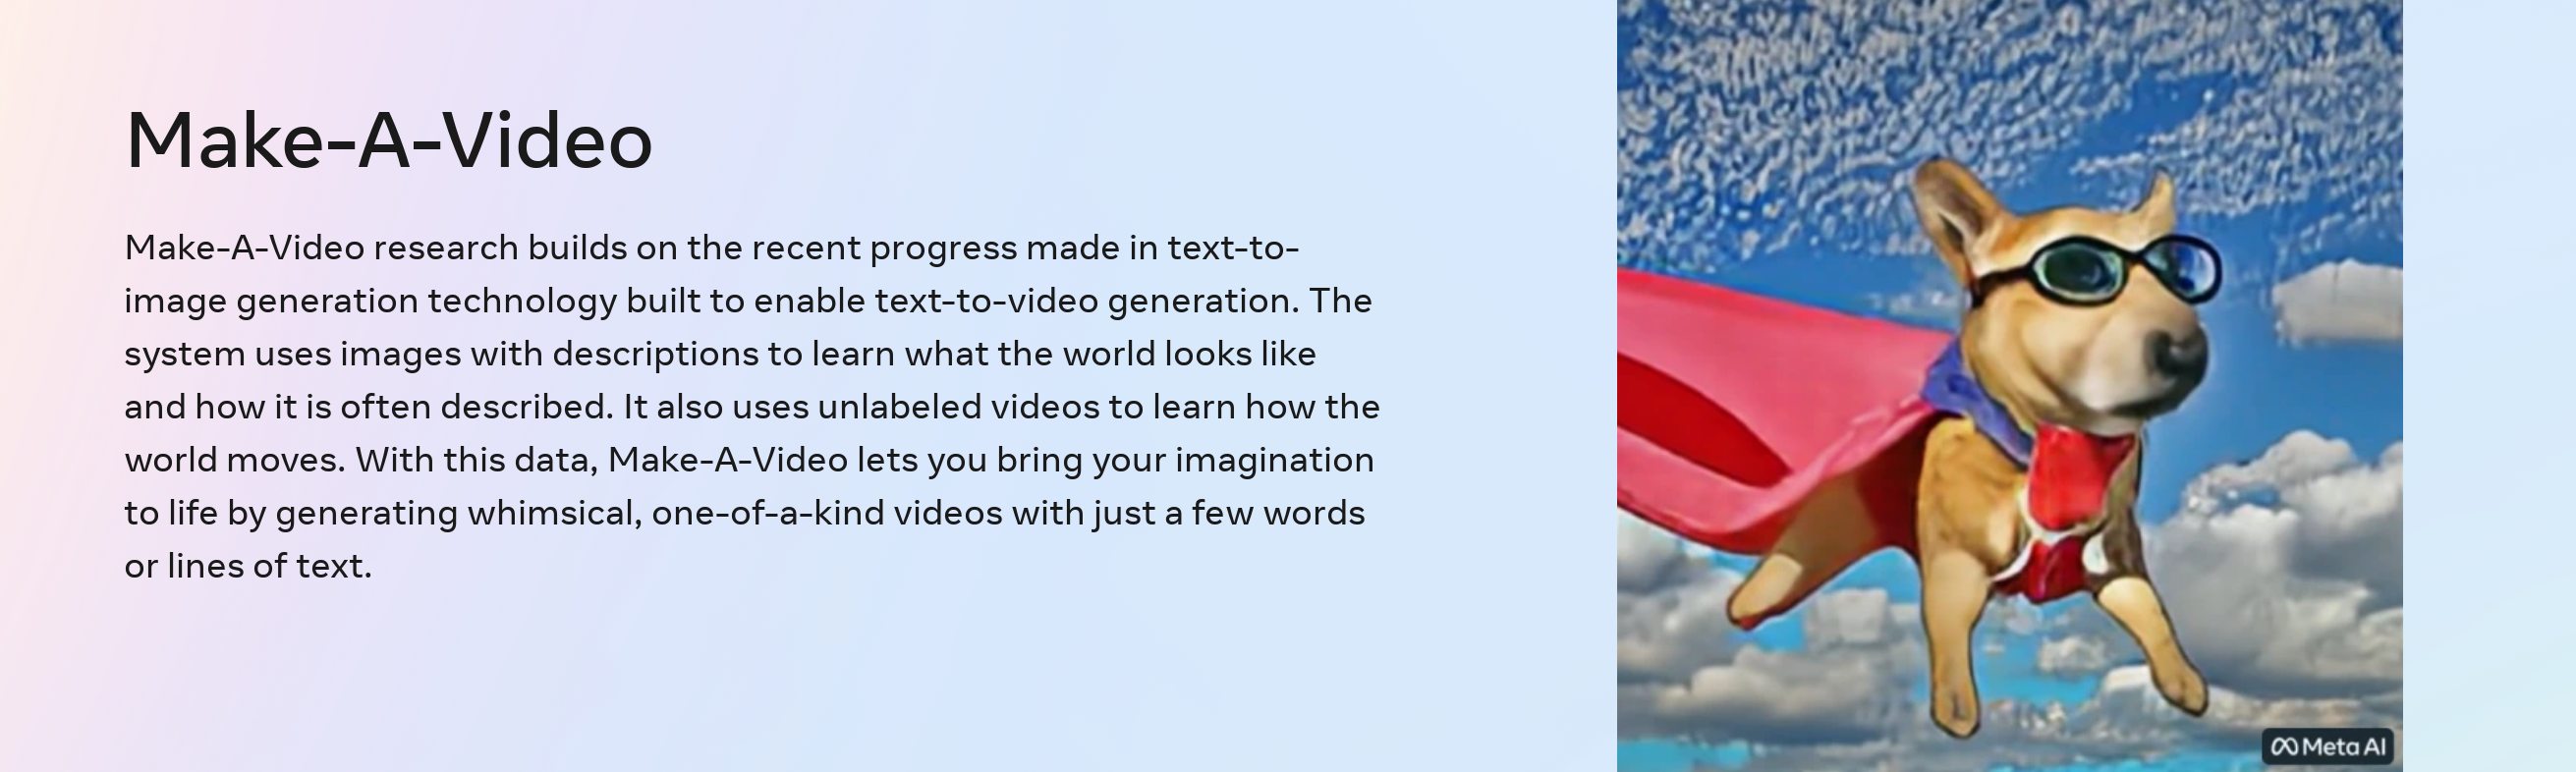
\includegraphics[width=9.5cm]{figs/makeavideo}
  \end{center}
  
  \begin{flushright}
    {\scriptsize
      \url{https://makeavideo.studio/}
    }
  \end{flushright}

  
\end{frame}


%%-----------------------------------------
%%-----------------------------------------
% \section{The future}

% %%-----------------------------------------
% \begin{frame}[fragile]
%   \frametitle{Assignments}

%   \begin{center}
%     
\includegraphics[width=7cm]{figs/kids-essays}
%   \end{center}

  
% \end{frame}

% %%-----------------------------------------
% \begin{frame}[fragile]
%   \frametitle{Programming}

%   \begin{center}
%     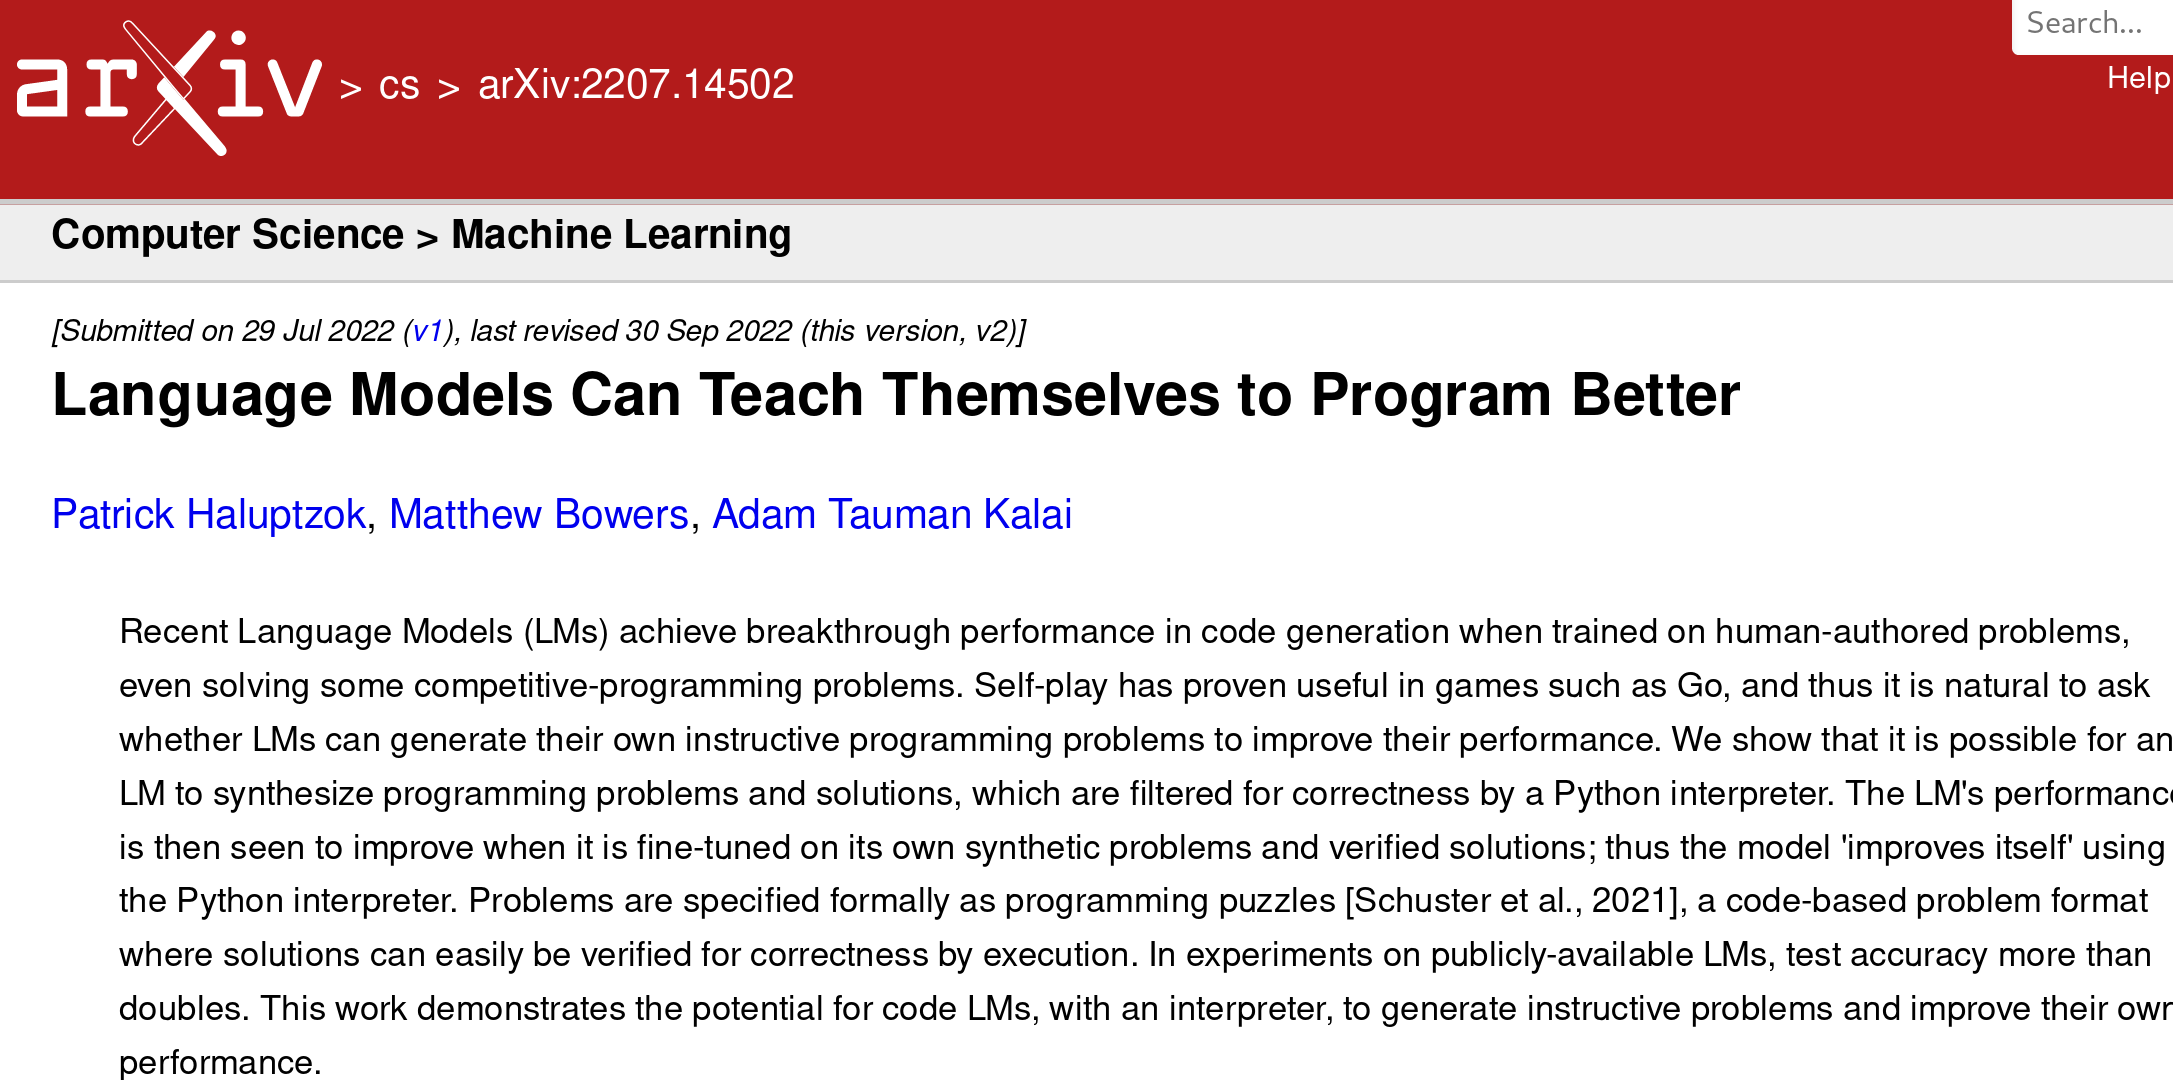
\includegraphics[width=10cm]{figs/llm-programming-better}
%   \end{center}

%   \begin{flushright}
%     {\small
%       \url{https://arxiv.org/abs/2207.14502}
%     }
%   \end{flushright}
  
% \end{frame}

% %%-----------------------------------------
% \begin{frame}[fragile]
%   \frametitle{Programming}

%   \begin{center}
%     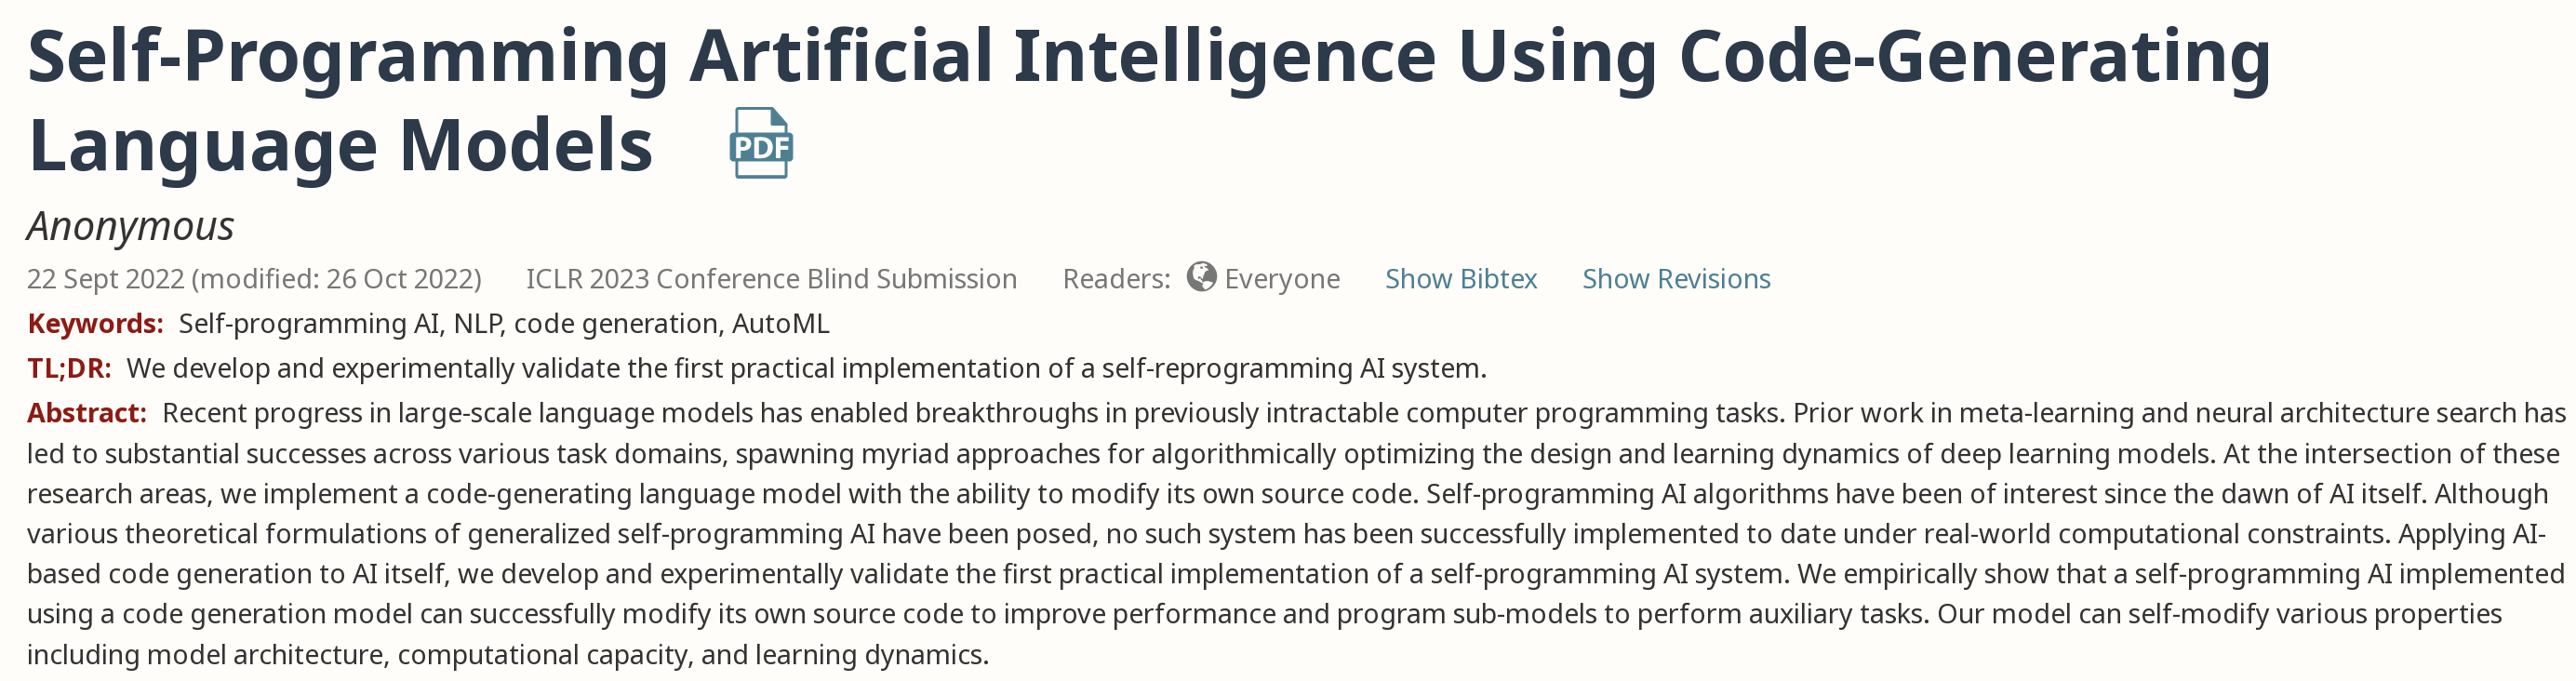
\includegraphics[width=10cm]{figs/self-programming}
%   \end{center}

%   \begin{flushright}
%     {\scriptsize
%       \url{https://keras.io/examples/generative/random_walks_with_stable_diffusion/}
%     }
%   \end{flushright}
  
% \end{frame}


%%-----------------------------------------
%%-----------------------------------------
\section{Summarizing}

%% -----------------------------------------
\begin{frame}[fragile]

  {\Large \bf
    The future just started
  }
\end{frame}


%%-----------------------------------------
%%-----------------------------------------
\section*{References}

% -----------------------------------------
\begin{frame}[fragile]

  {\huge References, credits, license}
\end{frame}

%% -----------------------------------------
\begin{frame}[fragile]
%  \frametitle{References}

  {\small
    \begin{itemize}
    \item Transformers-Tutorials \\
      {\scriptsize \url{https://github.com/NielsRogge/Transformers-Tutorials}}
    \item Vision Transformers \\
      {\scriptsize \url{https://cameronrwolfe.substack.com/p/vision-transformers}}
    \item A walk through latent space with Stable Diffusion \\
      {\scriptsize \url{https://keras.io/examples/generative/random_walks_with_stable_diffusion/}}
    \item How Open Source is eating AI \\
      {\scriptsize \url{https://lspace.swyx.io/p/open-source-ai}}
    \end{itemize}
  }  
\end{frame}

%% -----------------------------------------
\begin{frame}[fragile]
%  \frametitle{References}


  {\small
    \begin{itemize}
    \item Awesome Diffusion Models \\
      {\scriptsize \url{https://github.com/heejkoo/Awesome-Diffusion-Models}}
    \item /r/StableDiffusion at Reddit \\
      {\scriptsize \url{https://www.reddit.com/r/StableDiffusion}}
    \item The Generative Landscape (WiP course) \\
      {\scriptsize \url{https://johnowhitaker.github.io/tglcourse/}}
    \end{itemize}
  }  
\end{frame}

% -----------------------------------------
\begin{frame}[fragile]
  \frametitle{Credits}

  
\includegraphics[width=1.5cm]{figs/bookpages}
  {\small \href{https://pixabay.com/en/book-reading-library-literature-1261800/}{Book}, by NikolayFrolochkin, Pixabay. \\ License: Creative Commons CC0\\}

\end{frame}



\frame{
~
\vspace{1cm}

\begin{flushright}


\includegraphics[width=2.2cm]{figs/by-sa}
 \\

\begin{footnotesize}
\copyright 2022-2024 Jesus M. Gonzalez-Barahona. \\

\vspace{.4cm}

Some rights reserved. This document is distributed under the terms of the Creative Commons License ``Attribution-ShareAlike 4.0'',
available in \\
{\scriptsize \url{http://creativecommons.org/licenses/by-sa/4.0/}} \\

\vspace{.4cm}

This document (including source) is available from
\url{https://jgbarah.github.io/presentations}

\end{footnotesize}
\end{flushright}

}
%%

%\againframe{firstframe}

\end{document}

%%% Local Variables:
%%% mode: latex
%%% TeX-master: t
%%% End:
